\documentclass[11pt]{report} % Use report class for chapters
\usepackage[a4paper, top=2cm, bottom=2cm, left=2cm, right=2cm]{geometry}
\usepackage{amsmath, amssymb} % For math formatting
\usepackage{titlesec} % For customising section titles
%\titlespacing{\chapter}{0pt}{-30pt}{20pt} % Adjust top spacing
\usepackage{fancyhdr} % For headers and footers
\usepackage{hyperref} % For a clickable table of contents and references
\usepackage{tocloft} % For customising the table of contents
\usepackage{setspace} % For line spacing
\usepackage{booktabs}
\renewcommand{\abstractname}{Acknowledgement} % Change "Abstract" to "Summary"

% Formatting title sections
\titleformat{\chapter}[hang]{\bfseries\LARGE}{Chapter \thechapter}{1em}{}
\titleformat{\section}[hang]{\large\bfseries}{\thesection}{1em}{}

% Customise TOC spacing
\renewcommand{\cftchapdotsep}{1.5} % Adjust dots in TOC

% Line spacing
%\onehalfspacing % Set 1.5 line spacing
\setstretch{1.1}  % or any number like 1.25, 1.4, etc.

% Header and footer
\pagestyle{fancy}
\fancyhf{}
\fancyhead[L]{\slshape \leftmark} % Chapter title on left
\fancyfoot[C]{\thepage} % Page number at center

% Math and Symbols
\usepackage{amsmath, amssymb} % For math environments and symbols

% Graphics and Floats
\usepackage{graphicx} % Include images
\usepackage{float} % Improved float handling

% Hyperlinks
\usepackage{hyperref} % For clickable hyperlinks

% Code Listings
\usepackage{listings}
\usepackage{xcolor}

\lstset{
    language=R,                     % Set language to R
    basicstyle=\ttfamily\Huge,      % Increase font size (change to Huge, Large, normalsize)
    breaklines=true,                 % Enable automatic line breaking
    breakatwhitespace=true,          % Allow line breaks at spaces
    keepspaces=true,                 % Keep spaces in text
    columns=fullflexible,            % Fix alignment
    frame=single,                    % Adds a frame around the code
    backgroundcolor=\color{gray!10},  % Light gray background for readability
    keywordstyle=\color{blue},        % Blue for function names
    commentstyle=\color{green!50!black}, % Green for comments
    stringstyle=\color{red},          % Red for strings
}

% Citations
\usepackage[numbers, super]{natbib} % For citation styles
% Remove \usepackage{cite}, as natbib replaces it.

% Images
\usepackage{subcaption}
%\captionsetup[subfigure]{font=scriptsize}
\captionsetup[figure]{font=small}

\usepackage{xfp} % For calculations in LaTeX
\usepackage{xcolor} % For color coding

\definecolor{darkgreen}{rgb}{0.0, 0.5, 0.0}
\definecolor{lightgreen}{rgb}{0.0, 0.75, 0.0}
\definecolor{yellow}{rgb}{1.0, 0.84, 0.0}
\definecolor{red}{rgb}{1.0, 0.0, 0.0}

\newcommand{\classifyFit}[1]{%
  \ifnum\fpeval{#1 <= 0.5}=1 \textcolor{darkgreen}{Excellent}% 
  \else\ifnum\fpeval{#1 <= 0.6}=1 \textcolor{lightgreen}{Good}% 
  \else\ifnum\fpeval{#1 <= 0.7}=1 \textcolor{yellow}{Satisfactory}% 
  \else \textcolor{red}{Unsatisfactory}% 
  \fi\fi\fi
}

\lstset{
    language=R,
    basicstyle=\ttfamily\scriptsize, % Use smaller font size
    flexiblecolumns=true,            % Allows font to shrink for long lines
    showstringspaces=false,          % Do not show spaces in strings
    frame=none,                      % No frame around code
    numbers=none,                    % No line numbers
    breaklines=false,                % Force code in one line
    literate={~}{{\texttildelow}}1
}

% Begin document
\begin{document}


\begin{titlepage}
    \begin{center} 
        \hfill \break
         \vspace{5mm}
         
        
\includegraphics[width=0.6\textwidth]{Images/Durham_Uni_Name.png}   
       
        \vspace{1cm}
        \LARGE
            Department of Mathematical Sciences \\
            Project IV - (MATH4072)
        
        \linethickness{0.5mm}
        \Huge
            \line(1,0){250}\\
            \textbf{Equity Fund Profitability and Sustainability Modelling}\\
            %\line(1,0){250}

        \vspace{0.3cm}
        \LARGE
        \textit{Using Multiple-Response Regression}  % Subtitle added here
        \line(1,0){250}
        \vspace{1cm}
        
    \end{center}  

    \begin{minipage}[t]{0.47\textwidth}\centering
        {\Large \textbf{Author}:\\
        Raul Unnithan}\\
    \end{minipage}
    \hfill
    \begin{minipage}[t]{0.47\textwidth}\centering
        {\Large \textbf{Supervisor}:\\
        Ric Crossman}
    \end{minipage}

    \vfill  % Pushes date to the bottom

    \begin{center}
        \large \today  
    \end{center}
    
\end{titlepage}

\begin{abstract}
I would like to sincerely thank Ric for his support and guidance, both as my dissertation supervisor and throughout my time at Durham as my academic advisor. His advice and encouragement have been instrumental in guiding this project and in completing my academics at university. 
\end{abstract}

\renewcommand{\abstractname}{Declaration} % Change "Abstract" to "Summary"

\begin{abstract}
This piece of work is a result of my own work and I have complied with the Department’s guidance on multiple submission and on the use of AI tools. Material from the work of others not involved in the project has been acknowledged, quotations and paraphrases suitably indicated, and all uses of AI tools have been declared.
\end{abstract}


\tableofcontents

\chapter{Introduction}
\section{Background}
\subsection{Multiple-Response Regression}
Single-response regression models one response against a set of predictor variables. This method can be extended to multiple predictors, but what if more than one response needs to be modelled? One approach is to run several independent single-response models. However, this approach can lead to suboptimal predictions as it ignores that when responses are correlated, the off-diagonal elements of the response-covariance matrix are non-zero. Multiple-response regression (MRR) addresses this issue, thereby improving predictions. 

However, selecting the most relevant predictors remains a challenge, and each MRR model does this differently. This report has examined and applied different MRR models to an equity fund dataset to determine which of these fits it the best.

\subsection{Equity Funds}
An equity fund is a pooled investment that puts money predominantly in stocks listed on major exchanges.\cite{Chen2024EquityFunds}
They provide investors with several benefits, such as diversification and potential improved returns, but they also come with risks associated with stock market volatility and losses.\cite{Chen2024EquityFunds}
Equity funds can be categorised according to factors such as their investment style and portfolio focus, where a portfolio is the collection of stocks held by the fund, which is how they are represented in this data.\cite{Chen2024EquityFunds}

\section{Equity Fund Dataset}
\subsection{Overview}
The equity fund dataset analysed in this report contains information about a diverse range of funds, with varying equity fund characteristics, including, for example, the type of equity. Modelling equity fund data is important as it can indicate which funds are worth investing in and which are not. 

Traditional financial models prioritise profitability above all else.\cite{KumarSus} However, this report extends this by modelling two responses, with moderate correlation. These responses are return on equity (ROE) and sustainability score. At least a moderate correlation between responses is important here, as otherwise it would be more appropriate to model each response separately. 

\subsection{ROE and Sustainability Score}
ROE is a measure of an equity fund's profitability and how efficiently it generates those profits.\cite{fernando2023return} It is calculated by dividing net income by shareholders' equity.\cite{fernando2023return} ROE is typically expressed as a percentage, so this value is multiplied by a hundred. In the context of an equity fund, net income is not derived from sales minus the cost of goods sold as it would be for a company.\cite{kenton2024netincome} Instead, an equity fund’s net income comes primarily from earnings such as interest, after subtracting operating expenses like distribution costs.\cite{kenton2024netincome} The higher the ROE, the more efficiently an equity fund is generating income from its stocks it has invested in.\cite{franklin2019principles}

The sustainability score measures an equity fund’s sustainability performance and how effectively it mitigates environmental, social, and governance (ESG) risks across its portfolio. Each equity fund's sustainability score is its Morningstar Sustainability Rating, which directly measures these ESG factors.
The Morningstar Sustainability Rating is calculated through a multi-step process. First, a fund only qualifies for a rating if at least 67\% of its assets have an assigned ESG score.
Each company within the fund’s portfolio is then scored, typically on a scale from 1 to 100. The fund’s portfolio score is adjusted by subtracting points for any ESG-related negative events, such as environmental incidents. Finally, the equity fund's overall sustainability score is then compiled as a weighted average over the past 12 months, placing more emphasis on recent performance.\cite{chen2023morningstar} Lower sustainability scores indicate better ESG performance. 

\subsection{Motivation}
Modelling specifically ROE and sustainability scores in particular together is important as it gives a more long-term view of each equity fund's risk versus return potential. Sustainability has become more relevant as investors move to prioritise sustainable portfolios. A key driver of this trend is the growing concern over climate change and global warming, which have significant long-term social and economic implications. In a 2021 letter to other CEOs, Larry Fink, the CEO of BlackRock, wrote that 81\% of a globally representative selection of BlackRock's sustainable indexes outperformed their parent benchmarks.\cite{Fink2021Letter} This finding emphasises the importance of considering sustainability metrics alongside profitability measures when evaluating financial assets, including equity funds.

\section{Small-Scale Dataset}
Every MRR model in this report generated predictions for the two responses. These predictions were evaluated using the average normalised root mean square error, which is the root mean square error divided by the standard deviation averaged across each response (see Subsection~\ref{model measurement} for more). 

Each MRR model was also applied to a small-scale dataset with Exam Scores to demonstrate explicitly how these models make predictions:
\setlength{\tabcolsep}{3pt} % Adjust column spacing
\begin{table}[H]
    \centering
    \begin{tabular}{|c|c|c|c|}
        \hline
        \( X_1 \): Hours Studied & \( X_2 \): Time Spent on Papers & \( Y_1 \): Math Scores & \( Y_2 \): Science Scores\\
        \hline
        5  & 2  & 78 & 80 \\
        7  & 3  & 85 & 79 \\
        8  & 4  & 88 & 88 \\
        3  & 1  & 65 & 70 \\
        10 & 5  & 92 & 74 \\
        \hline
    \end{tabular}
    \caption{Study Time vs. Exam Scores}
    \label{tab:study_scores1}
\end{table}
\noindent The calculations involving this dataset used precise values throughout, but, where written, the intermediary and final results were rounded to 2 decimal places for brevity - unless explicitly stated otherwise. The Exam Scores dataset was used for this purpose because its values are straightforward, and the responses have a moderate correlation of 0.526 (3dp), indicating that it requires MRR (see Subsection~\ref{Math Sci Cor} for the full calculation). 

\section{Report Terminology}
In this report, certain common terminology was used. First, the identity matrix was denoted throughout as $\mathbf{I}$ with dimensions subscripted where necessary. Second, there was the correlation and covariance between the responses, which, as stated, MRR considers unlike single-response regression. This consideration is essential for every MRR model as it is what qualifies them as multiple-response. 

The correlation between the responses, referred to as the response intercorrelation, was defined as a matrix, $\mathbf{R}$, using the formula: 
$
\mathbf{R} = \mathbf{D}^{-1} \mathbf{\Sigma_Y} \mathbf{D}^{-1},
$ %\vspace{0cm}
\noindent where \( \text{Cov}(\mathbf{Y})=\mathbf{\Sigma_Y} \) denotes the covariance matrix of the response variables, or the response covariance matrix, and \( \mathbf{D} \) is a diagonal matrix of the standard deviations of the response variables.\cite{mardia2024multivariate}
Each element of \( \mathbf{R} \) is computed as: %\vspace{-0.1cm}
\[
    R_{ij} = \frac{(\mathbf{\Sigma_Y})_{ij}}{\sigma_i \sigma_j},
\] %\vspace{0cm}
where \( (\mathbf{\Sigma_Y})_{ij} \) is the covariance between response variables \( i \) and \( j \), and \( \sigma_i, \sigma_j \) are their respective standard deviations.\cite{mardia2024multivariate}
This relation ultimately means that if an MRR model considers the off-diagonal elements in the response covariance matrix, it considers the response intercorrelation and vice versa. 

\section{Report Outline}
The rest of this report is broken down into chapters containing the exploratory data analysis, the MRR models and a conclusion comparing every model's performance.

Chapter 2 covers an Exploratory Data Analysis of the equity fund dataset. The master dataset includes equity and bond funds with a lot of missing data. This chapter focuses on cleaning and refining the dataset, defining the predictor variables,  applying imputation techniques to address missing data, and understanding the relationship between the two responses: ROE and sustainability score.

Chapter 3 introduces Multiple-Response Linear Regression. It delves into its underlying theory and explains how it can be combined with multiple analysis of variance and stepwise selection to select appropriate predictors. These stepwise selection methods are evaluated on the equity fund dataset.

Chapter 4 progresses to shrinkage-based regression methods. It looks at more advanced methods appropriate for MRR, including Multivariate Regression with Covariance Estimation and Reduced Rank Ridge Regression. These methods are again evaluated, and their performance is assessed to determine whether they offer improvements over the MRLR models.

Chapter 5 introduces non-linear modelling through Random Forests. It extends them to MRR using Covariance Regression with Random Forests, and then applies the resulting model to the dataset.

Chapter 6 continues the non-linear modelling approach using XGBoost. It also outlines Cholesky Decomposition, which enables XGBoost to be used in MRR. The resulting Cholesky Decomposition XGBoost model is then evaluated on the equity fund dataset.

Finally, Chapter 7 gives an overall comparison of the performance of each modelling approach applied. It identifies the most effective method for predicting ROE and sustainability scores based on the findings, discusses challenges and limitations throughout the report, and looks into potential directions for future work.

\chapter{Exploratory Data Analysis}
\label{EDA}
This chapter prepares the equity fund dataset for modelling. It begins by describing the master dataset and the initial preprocessing steps taken to remove irrelevant variables. The key predictor variables in the partially cleaned dataset are then explained. Exploratory data analysis follows, including an assessment of the distributions of the responses and the correlation structure among the predictors. Imputation is subsequently applied to complete the dataset, facilitating multicollinearity testing. Finally, this chapter examines the intercorrelation between the responses, tests the assumption of multivariate normality, and explores the relationship between the responses in greater depth.

\vspace{-0.2cm}
\section{Initial Data Collection and Preprocessing}
The dataset was obtained from Kaggle and simplified for this analysis. This report focuses on analysing equity funds, but the master dataset contains a mixture of equity and bond funds. 

The first step was to filter out the bond funds and keep the equities. This filtering was done using Excel's filter features. A text filter was used to select the relevant rows within the \texttt{category} column. 

Next, there was an issue with the columns because there were 130 dependent variables in this intermediary dataset. However, because many variables were for bonds only, these were removed. Some variables, such as a fund's \texttt{isin} number, were irrelevant for analysis, further reducing the number of dependent variables to 29. 

Because it was critical to be able to look into how chosen predictors would affect the responses, the aim was to have 10-20 predictors in the model as this is a manageable amount. Also, a lot of the remaining variables served the same purpose, which would lead to multicollinearity. For example, \texttt{management\_fees} was removed because it is a significant component of \texttt{ongoing\_cost}.

\vspace{-0.2cm}
\section{Variable Explanation}
\texttt{category} gives the type of each equity fund. The cleaned equity fund dataset contained 91 unique equity types, consisting of country equities, such as \texttt{"Italy Equity"}, and sector equities, such as \texttt{"Sector Equity Precious Metals"}. Sector equity funds invest in firms in a specific sector or industry, such as technology, regardless of a company's country of operation. However, country equity funds invest in firms with extensive operations in a specific country, regardless of the industry or sector. 

A \texttt{rating} is given by analysts assigned to the equity fund, and this takes values \{1, 2, 3, 4, 5\}. In Category 1, funds have excellent performance and high returns relative to their risk of investment. Category 2 includes funds with a solid performance and risk versus return performance, though not as good as Category 1. Category 3 includes funds that are fairly valued and perform in line with market averages, and investors are advised to hold their positions. Category 4 includes funds that underperform their peers. Lastly, Category 5 represents funds that underperform over the long term and are higher risk, meaning they should be withdrawn from.

An equity's \texttt{risk\_rating} is a metric of its market volatility.\cite{stockopedia2024} \texttt{risk\_rating} takes the same values as \texttt{rating} but measures the risk of investing in an equity fund. Category 1 funds are less volatile and more stable, and thus are suitable for conservative investors. Category 2 funds are moderately volatile but still reasonably safe. Category 3 funds have medium volatility, balancing risk and potential returns. Category 4 funds are more volatile, with a greater possibility of returns as well as greater exposure to market volatility. Lastly, Category 5 funds are subject to the highest risk and volatility.

\texttt{rating}, and \texttt{risk\_rating} are ordinal variables as they exhibit an order by definition. \texttt{category} is a categorical variable because it represents different non-numeric groupings; here, these are countries and sectors, which do not have a natural order.\cite{james2021islr} The rest of the variables are continuous.

\texttt{equity\_style\_score} is the difference between two investment strategies: growth and value stocks.\cite{amg2023} Growth stocks are expected to bring in a lot of capital due to strong growth in the underlying company.\cite{hayes2023} Value stocks are either underrated or ignored by the market, and they could gain value eventually.\cite{hayes2023} Therefore, a lower \texttt{equity\_style\_score} means the stock is more of a value stock, and a higher \texttt{equity\_style\_score} indicates more of a growth stock.
\texttt{equity\_size\_score} measures the performance of said equity relative to the company's value.\cite{adatiya2022} \texttt{price\_prospective\_earnings} gives the ratio between a company's share price and earnings per share. \texttt{price\_cash\_flow\_ratio} is a ratio that compares a company's market value to the amount of money it generates during a select period.\cite{adatiya2022}

A dividend is the money companies might decide to pay you if you own their shares, and the dividend yield is the dividend paid as a percentage of the share price. The \texttt{dividend\_yield\_factor}	is the dividend yield, except it is used to compare the different equities, considering variations in dividend yield performance. \texttt{historical\_earnings\_growth} measures how a stock's earnings per share have grown in the last 5 years. \texttt{sales\_growth} is the increase in sales of a company's products/ services over time. \texttt{asset\_cash} is the proportion of a fund's assets held in cash. \texttt{holdings\_n\_stock}	is the number of different stock holdings each equity fund holds. A stock holding is the number of other companies which the equity fund has invested in by holding their stocks. \texttt{ongoing\_cost} is the cost of the daily running of a business.\cite{murphy2024_operating_costs}	\texttt{fund\_size} is the sum of all the assets in the fund.
\vspace{-0.2cm}
\section{Exploratory Data Analysis}
Now that the dataset was cleaned and the variables specified and defined, the next step was to perform data analysis in R and find underlying relationships between the variables. To fully represent the dataset, it is best to use actual values rather than simulate any missing values. So, this initial analysis was done with only rows with no missing values.
\vspace{-0.3cm}
\subsection{Underlying Distributions}
QQ plots indicate if a variable is normally distributed. These are shown below for the responses:
\begin{figure}[H]
    \centering
    % First image
    \begin{minipage}[b]{0.38\textwidth}
        \centering
        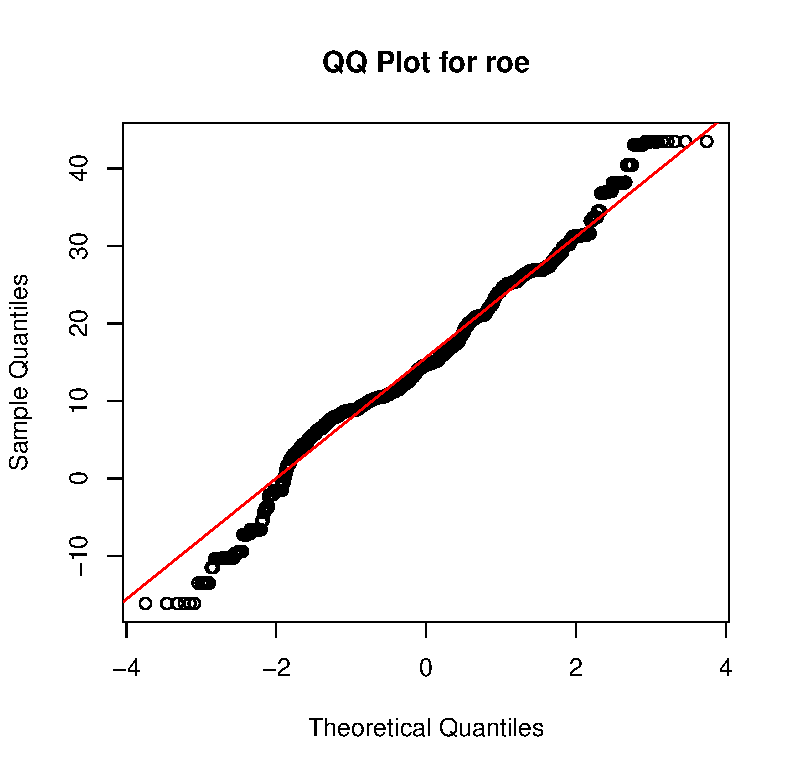
\includegraphics[width=\textwidth]{QQ Plot for ROE.pdf} % Replace with your image path
    \end{minipage}
    \hfill
    % Second image
    \begin{minipage}[b]{0.4\textwidth}
        \centering
        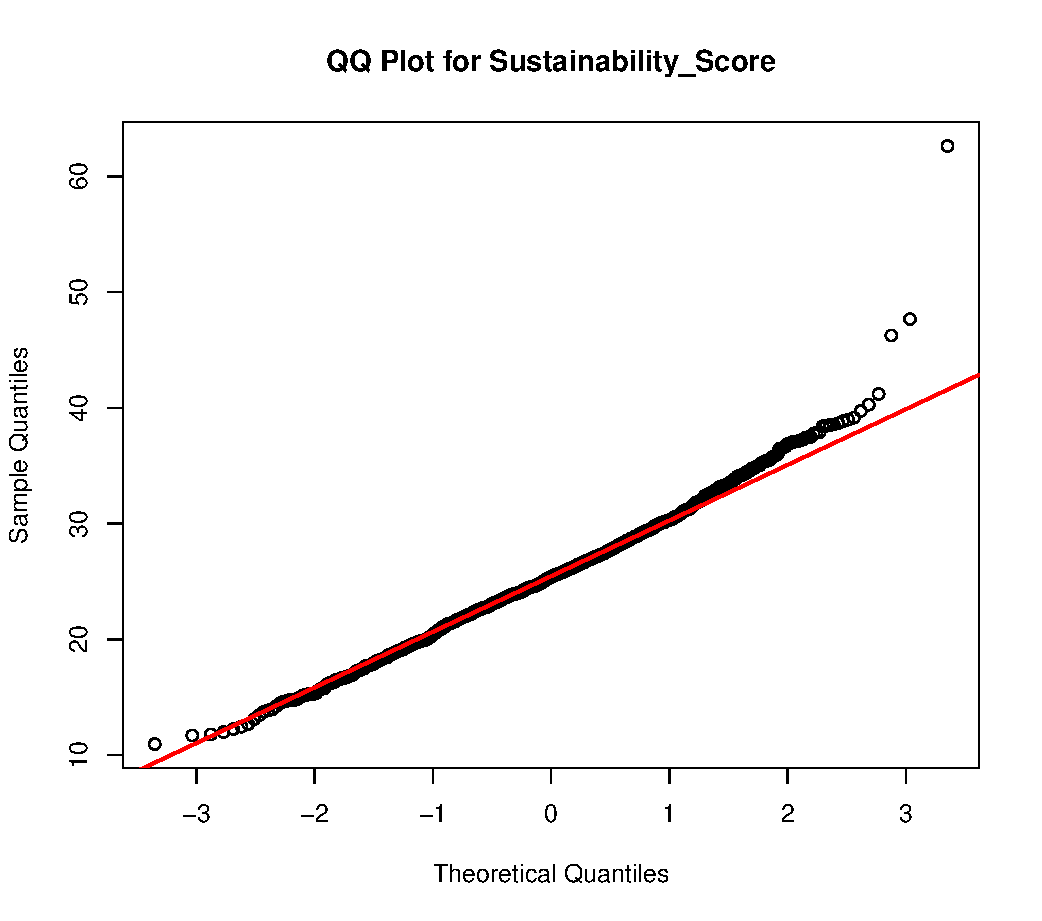
\includegraphics[width=\textwidth]{QQ Plot for Sustainability_Score.pdf} % Replace with your image path
    \end{minipage}
    \caption{QQ Plots for ROE and Sustainability Scores}
    \label{fig:sidebyside_minipage}
\end{figure}

\noindent From the QQ Plots above, there is strong evidence that ROE and sustainability score are normally distributed because the points on the QQ plot approximate a straight line.

\vspace{-0.3cm}
\subsection{Correlation}
\label{Correlation and Multi-Collinearity}
It was also essential to examine the correlation among the predictors to determine whether any should be removed. High correlation implies multicollinearity, so this was checked before proceeding. After creating the correlation matrix for the predictors, there were two high correlation values. One high correlation, \( 0.8099 \), was observed between \texttt{price\_prospective\_earnings} and \texttt{price\_cash\_flow\_ratio}. Based on the definitions of these variables, the latter was judged to align more closely with profitability and sustainability and was therefore retained.
Similarly, a high negative correlation of \( -0.8029 \) was identified between \texttt{dividend\_yield\_factor} and \texttt{equity\_style\_score}. Here, \texttt{dividend\_yield\_factor} was considered a more relevant factor. After these adjustments, 12 predictors remained.

\vspace{-0.3cm}
\subsection{Imputing Missing Values}
Although high correlation implies multicollinearity, the opposite is not necessarily true because multicollinearity is not just about pairwise relationships. Multicollinearity arises from predictor linear dependence. For instance, if Variable $A$ is a linear combination of Variables $B$ and $C$, say $A = 2B + C$, multicollinearity can occur even if there is no high pairwise correlation.\citep{kutner2005applied} 
Therefore, methods such as the Variance Inflation Factor (VIF) are used to detect multicollinearity beyond correlation.\citep{belsley1980regression} 

% However, this dataset contains a mixture of categorical and continuous variables, so it is necessary to consider both variable types in the VIF analysis.

The dataset should also be complete before carrying out a VIF analysis. The first step to ensuring completeness involves analysing how the NA values are spread and how often they occur in each row. It was found that 90\% of the rows had two NA entries or less, and because the dataset is large, only these rows were used in further analysis. There were three types of missing data here corresponding to the numerical, categorical and ordinal variables that needed to be imputed.

Random forest imputation was used to fill in the missing categorical and ordinal data for several reasons. Although it is computationally more expensive than using methods such as the mode to fill in missing data, it deals well with variables with no association. The Spearman's Rank test confirmed this relationship between the ordinal variables, rating and risk rating. It gave an association of -0.0728, indicating there was sufficient evidence to suggest a lack of association between them.

Random forest imputation also works for categorical and ordinal data through surrogate splits, and outliers influence them less as they use an ensemble of decision trees. Random forest imputations also do not require prior assumptions of the underlying distribution, making them more flexible than methods such as linear model imputation, which requires underlying distribution normality.\cite{hong2020randomforest} 

The random forest model was trained on rows with no NA values and was set to make sure it was predicting categorical and ordinal values rather than numerical ones. Ultimately, the model learned the relationships between the target variable it was imputing and the other columns in the dataset. 

Linear model imputation was used to fill in missing numerical features because it uses the relationships between variables rather than relying on simpler approaches such as mean imputation. This method assumes that each response variable is drawn from an underlying normal distribution, and this is supported by the Q-Q plots shown in Figure~\ref{fig:sidebyside_minipage}.\cite{Salgado2016}

In the linear model, the ordinal predictors, which have integer values from 1 to 5, were used as numerical predictors as they have roughly equal spacing among levels.\cite{openfunds2020} However, the categorical predictor, \texttt{category}, was frequency encoded to prevent it from imposing a hierarchy in the model. 

\vspace{-0.3cm}
\subsection{Multicollinearity}
\label{Multicollinearity}
VIF analysis was employed using a multiple-response linear regression model of the responses against the features (see Section~\ref{MRLR Section} for more on this), where \texttt{category} was frequency encoded. Following this, a dummy response was added for VIF calculation, and the VIF values were derived from this new model. 
If any predictors had VIF values greater than 10, they would have been removed due to multicollinearity. Here, however, all VIF values were below 5 (see Figure~\ref{fig:vif} for confirmation of this). Therefore, none of the predictors exhibited multicollinearity and hence, they were all retained.

\noindent Finally, this left a cleaned equity fund dataset with 1248 rows, each with individual equity fund information. In addition, there were 14 columns, with 2 response variables and 12 predictors.
\vspace{-0.2cm}
\subsection{Multivariate Normality}
\label{Multivariate Normality}
Many of the MRR models in this report relied on the assumption of response multivariate normality. This was evaluated using Mardia’s test, which assesses multivariate skewness and kurtosis.
The null and alternative hypotheses of Mardia's test are that the responses are and are not multivariate normally distributed, respectively. Therefore, if either the kurtosis or skewness statistic deviates significantly from their expected values under multivariate normality, then the null hypothesis is rejected.\cite{mardia2024multivariate} 

Mardia's test returned p-values of 0.0732 for skewness and 0.0862 for kurtosis, meaning that in both cases, we failed to reject the null hypothesis of multivariate normality at a 5\% significance level. Therefore, there was sufficient evidence to suggest a multivariate normal assumption for the responses (see Subsection~\ref{Mardia's Test for MVN} for more on how these p-values were derived).

However, the relatively low p-values suggested that the assumption may not hold perfectly, and this mild deviation from normality helped explain differences in performance between models that require distributional assumptions and those that do not.
\vspace{-0.2cm}
\section{Response Intercorrelation}
As stated in the introduction, considering response intercorrelation is what separates MRR from single-response regression. If the dataset consisted of response variables which shared no correlation, one model could be built for each response, and MRR would not be needed.

Before proceeding with each MRR model, it was worth briefly examining the relationship between the two response variables: ROE and sustainability score. Figure~\ref{fig:ROESUS} shows a scatter plot of these responses, with a fitted regression line included to highlight their correlation:
\begin{figure}[H]
    \centering
    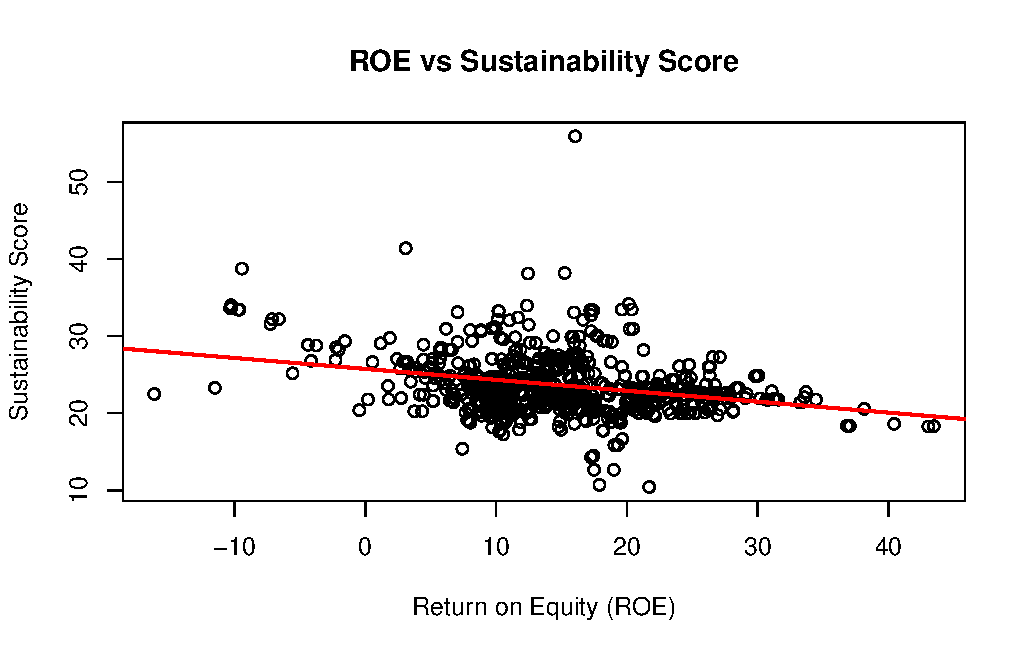
\includegraphics[width=0.5\linewidth]{ROESUS.pdf}
    \caption{Scatter Plot of Return on Equity vs. Sustainability Score}
    \label{fig:ROESUS}
\end{figure}
\noindent The regression line above shows a slight negative slope, indicating a negative correlation between ROE and sustainability score. Using the \texttt{cor} function in R gives a response correlation of \texttt{-0.313} (to 3sf). This correlation means that, generally, as ROE increases, the sustainability score decreases.

Here were the full empirical covariance and correlation matrices between the responses (to 3sf):
\[
\mathbf{R} =
\begin{pmatrix}
1.00 & -0.313 \\
-0.313 & 1.00
\end{pmatrix},
\quad
\mathbf{\Sigma_Y} =
\begin{pmatrix}
62.0 & -8.79 \\
-8.79 & 12.7
\end{pmatrix}.
\]
The negative correlation and covariance might be surprising given current trends toward a more sustainable climate. However, a lower sustainability score means an equity fund is a more sustainable option, so this does follow the expected trend.



\chapter{Linear Regression}
\label{C3}
This chapter introduces the methodology of the first MRR model, multiple-response linear regression, by starting with single-response linear regression. Stepwise selection methods are then introduced, followed by an explanation of how they can be extended to consider multiple responses, using the multiple analysis of variance, to determine which predictors are included in the multiple-response models. The accompanying code will then be explained, and the models in this chapter are evaluated using the average normalised root mean square error.

\section{Theory}

\subsection{Single-Response Linear Regression}
Before delving into multiple-response linear regression, let us start with single-response linear regression (SRLR). SRLR models the relationship between one response variable and a set of predictor variables. The general form of this model, with the dimensions subscripted, is:
\begin{equation}
\mathbf{Y}_{(n \times 1)} = \mathbf{X}_{(n \times p)} \boldsymbol{\beta}_{(p \times 1)} + \boldsymbol{\epsilon}_{(n \times 1)},
\label{SRLR}
\end{equation}
\noindent where $n$ is the number of observations, $p$ the number of predictors (including the column of ones), $\mathbf{Y}$ the response variable vector, $\mathbf{X}$ the design matrix, $\boldsymbol{\beta}$ the coefficient vector and $\boldsymbol{\epsilon}$ is the error variable vector. 

Including a column of ones in $\mathbf{X}$ adds an intercept term to the model. This is the expected response when all predictors are zero.

When modelling any data, the aim is to minimise the residuals. A residual is the difference between predicted and actual values, and reducing this ensures the model is as accurate as possible. This accuracy is achieved by finding the most optimal coefficient vector, $\boldsymbol{\beta}$. This optimal coefficient vector, also known as the ordinary least squares estimator (OLS), \( \boldsymbol{\hat{\beta}} \), is found by minimising the sum of squared residuals. It can also be defined using $\mathbf{X}$ and $\mathbf{Y}$ as follows:
\[
\boldsymbol{\hat{\beta}^{\text{OLS}}} = (\mathbf{X}^\top \mathbf{X})^{-1}\mathbf{X}^\top \mathbf{Y}.
\]
The model's accuracy can then be evaluated using metrics such as the $R^2$-value, which measures the proportion of variance in the dependent variable explained by the independent variables. 

SRLR comes with a few underlying assumptions, which relate to the properties of its error terms. They are linearity, homoscedasticity, normality, and independence of its variables. Linearity means there is a linear relationship between the dependent variables and the independent variables: \( E(Y_i | X_i) = \beta_0 + \beta_1 x_i \). The assumption of normality refers to the distribution of residuals, which are assumed to follow a normal distribution with mean zero and constant variance, $\sigma^2$. Homoscedasticity means that an even spread of residual values is expected, and the assumption that the model operates well for all values of the predictor variable holds. Finally, independence implies that the error covariance matrix is diagonal, and this is given by:
\begin{equation*}
    \text{Cov}(\boldsymbol{\epsilon}) = \sigma^2 \mathbf{I}_n,
\end{equation*}
where $\sigma^2$ is the true error variance. 

Since the true error variance, \( \sigma^2 \), is unknown, it is typically estimated from the residuals, 
\( \hat{\boldsymbol{\epsilon}} = \mathbf{Y} - \mathbf{X} \hat{\boldsymbol{\beta}} \), 
where \( \hat{\boldsymbol{\beta}} \) is the OLS estimator. An unbiased estimator of \( \sigma^2 \) is given by:
\begin{equation}
\hat{\sigma}^2 = \frac{1}{n - p} \hat{\boldsymbol{\epsilon}}^\top \hat{\boldsymbol{\epsilon}},
\label{unbiased}
\end{equation}
where $n$ is the number of observations and $p$ is the number of predictors. Therefore, because $\sigma^2$ can be estimated, the error covariance matrix, $\text{Cov}(\boldsymbol{\epsilon})$, can be too.
%It is also a necessary condition for the assumption that $\epsilon_i\sim\mathcal{N}(0,1)$ holds.
%This constant variance is also known as homoscedasticity, i.e. \(\text{Var}(y_i|x_i) = \sigma^2\), and it means variables are not too highly correlated.\cite{cfa2024mlr} Homoscedasticity, in turn, proves normality: \( Y_i | X_i \sim N(\beta_0 + \beta_1 x_i, \sigma^2) \). 

If this method were extended to model $m$ responses using $m$ independent single-response regression models, it would ignore the covariance between responses, leading to sub-optimal predictions when responses are correlated (see Equation~\ref{no off-diag} for a visual of this). 

However, SRLR can be extended to the multiple-response setting while incorporating this structure. This extended approach is known as multiple-response linear regression.

\subsection{Multiple-Response Linear Regression}
\label{MRLR Section}
Multiple-response linear regression (MRLR) is the most basic model in MRR. Its general form is:
\begin{equation}
\mathbf{Y}_{(n \times m)} = \mathbf{X}_{(n \times p)} \, \mathbf{B}_{(p \times m)} + \mathbf{E}_{(n \times m)},
\label{MRLR}
\end{equation}
with:
\[
E(e_{i}) = 0 \quad \text{and} \quad \text{Cov}(e_{i}, e_{k}) = \sigma_{ik} \mathbf{I}_n \quad i, k = 1, 2, \dots, m,
\]
where $n$ is the number of observations, $m$ is the number of responses, and $p$ is the number of predictors, including the column of ones, $\mathbf{Y}$ the response variable matrix, $\mathbf{X}$ the design matrix, $\mathbf{B}$ the coefficient matrix, and $\mathbf{E}$ is the error variable matrix. 

Including a column of ones in $\mathbf{X}$ allows the model to estimate an intercept for each response variable. These intercepts appear as the first row of the coefficient matrix, $\mathbf{B}$.
Like with SRLR, this represents the expected value of each response when all predictors are zero.

The first key difference between MRLR and SRLR lies in the structures of the responses, coefficients and errors. These are now matrices rather than vectors, reflecting that the responses are modelled together. 

As an example, suppose \( n = 4 \), \( p = 3 \), and \( m = 2 \), then the regression equation becomes:
\[
\mathbf{Y}_{(4 \times 2)} = \mathbf{X}_{(4 \times 3)} \, \mathbf{B}_{(3 \times 2)} + \mathbf{E}_{(4 \times 2)}.
\label{MRR_explicit}
\]
This expands to:
\[
\begin{aligned}
\begin{bmatrix}
y_{11} & y_{12} \\
y_{21} & y_{22} \\
y_{31} & y_{32} \\
y_{41} & y_{42}
\end{bmatrix}_{(4 \times 2)}
&=
\begin{bmatrix}
1 & x_{11} & x_{12} \\
1 & x_{21} & x_{22} \\
1 & x_{31} & x_{32} \\
1 & x_{41} & x_{42}
\end{bmatrix}_{(4 \times 3)}
\cdot
\begin{bmatrix}
b_{01} & b_{02} \\
b_{11} & b_{12} \\
b_{21} & b_{22}
\end{bmatrix}_{(3 \times 2)}
+
\begin{bmatrix}
e_{11} & e_{12} \\
e_{21} & e_{22} \\
e_{31} & e_{32} \\
e_{41} & e_{42}
\end{bmatrix}_{(4 \times 2)}.
\end{aligned}
\]
Each row in \( \mathbf{Y} \) corresponds to a single observation (i.e. a data point), and each column represents one of the \( m \) response variables. The coefficient matrix \( \mathbf{B} \) contains a separate column of regression coefficients for each response, and the error matrix \( \mathbf{E} \) captures the errors associated with each response for every observation.

The second key difference between SRLR and MRLR lies in the structure of the error terms. MRLR allows for correlation between errors across different responses within the same observation. This error covariance matrix captures this correlation:
\[ \mathbf{\Sigma_E} = \{\sigma_{ik}\}, \quad i, k = 1, 2, \dots, m,\] 
where \( \sigma_{ik} \) denotes the covariance between the error terms \( e_i \) and \( e_k \) associated with responses \( i \) and \( k \) in the same observation.\cite{johnson2013_chapter77} 

The sample error covariance matrix can be estimated using a formula analogous to the unbiased estimator of $\sigma^2$ in SRLR (from Equation~\ref{unbiased}):
\[
\mathbf{\hat{\Sigma}_E} = \frac{1}{n-p}\mathbf{E}^\top \mathbf{E},
\]
where $n$ is the number of observations and $p$ is the number of predictors.

For illustration, consider again the case where $n=4$, $p=3$ and $m=2$:
\begin{equation}
    \mathbf{\hat{\Sigma}_E} = \frac{1}{n-p}\mathbf{E}^\top \mathbf{E}=
\begin{bmatrix}
e_{11} & e_{21} & e_{31} & e_{41} \\
e_{12} & e_{22} & e_{32} & e_{42}
\end{bmatrix}
\begin{bmatrix}
e_{11} & e_{12} \\
e_{21} & e_{22} \\
e_{31} & e_{32} \\
e_{41} & e_{42}
\end{bmatrix}=
\begin{bmatrix}
\sum_{i=1}^{4} e_{i1}^2 & \sum_{i=1}^{4} e_{i1} e_{i2} \\
\sum_{i=1}^{4} e_{i1} e_{i2} & \sum_{i=1}^{4} e_{i2}^2
\end{bmatrix}.
\label{off-diag}
\end{equation}
If we used 2 independent single-response models, the off-diagonal elements of \( \mathbf{\hat{\Sigma}_E} \) would be 0. In this case, $\mathbf{\hat{\Sigma}_E}$ instead becomes:
\begin{equation}
    \mathbf{\hat{\Sigma}_E} =
\begin{bmatrix}
\sum_{i=1}^{4} e_{i1}^2 & 0 \\
0 & \sum_{i=1}^{4} e_{i2}^2
\end{bmatrix},
\label{no off-diag}
\end{equation}
which may lead to suboptimal predictions in the presence of correlated responses.

This error covariance structure is important as it qualifies MRLR as an MRR model. It does this because it is used to compute the sample response covariance matrix, \( \mathbf{\hat{\Sigma}_Y} \), as follows:
\begin{equation}
    \begin{aligned}
        \mathbf{\hat{\Sigma}_Y} = \text{Cov}(\mathbf{Y})&= \text{Cov}(\mathbf{XB} + \mathbf{E}) \\
        &= \text{Cov}(\mathbf{XB}) + \text{Cov}(\mathbf{E}) \\
        &= \mathbf{B}^\top \text{Cov}(\mathbf{X}) \mathbf{B} + \text{Cov}(\mathbf{E}) \\
        &= \mathbf{B}^\top \mathbf{\hat{\Sigma}_X} \mathbf{B} + \mathbf{\hat{\Sigma}_E},
    \end{aligned}
    \label{MRLR = MRR}
\end{equation}

\noindent where the linearity property of covariance justifies the first expansion (see Section~\ref{Covariance Expansion} for the simplification of Cov(\( \mathbf{XB} \)) to \( \mathbf{B}^\top \text{Cov}(\mathbf{X}) \mathbf{B} \)).

Equation~\ref{MRLR = MRR} shows that error interdependence remains, even after accounting for the predictors, and it is captured directly by the off-diagonal elements of \(\hat{\boldsymbol{\Sigma}}_{\mathbf{E}}\). Since \(\hat{\boldsymbol{\Sigma}}_{\mathbf{E}}\) appears explicitly in the expression for the response covariance matrix \(\hat{\boldsymbol{\Sigma}}_{\mathbf{Y}}\), modelling this structure is essential to capturing the covariance of the responses for MRLR.

Therefore, a non-zero value of the off-diagonal element of $\mathbf{\Sigma_E}$, \( \sigma_{ik} \), implies that responses \( i \) and \( k \) tend to vary together, suggesting interdependence between them.

MRLR comes with a few underlying assumptions, which can be extended from SRLR. Linearity comes from the formula for MRLR, which, when expanded, is:
\[
\begin{array}{rcl}
    Y_1 & = & b_{01} + b_{11}x_1 + \dots + b_{p1}x_p + e_1, \\
    Y_2 & = & b_{02} + b_{12}x_1 + \dots + b_{p2}x_p + e_2, \\
    \vdots & & \\
    Y_m & = & b_{0m} + b_{1m}x_1 + \dots + b_{pm}x_p + e_m.
\end{array}
\]
These rows are also independent, another MRLR property from SRLR.

\noindent Normality also holds here, but it differs slightly. If we look at using several independent single-response models, each error term is independent and identically normally distributed, with $\epsilon_i \sim \mathcal{N}(0,\mathbf{I})$. However, in MRLR, the error terms, \( \mathbf{E} \), share the same distribution. They are assumed to have a multivariate normal distribution with constant variance: $\mathbf{E} \sim \mathcal{N}_m(\mathbf{0}, \mathbf{\Sigma_E})$, where \(\mathbf{\Sigma_E} \) is the covariance matrix of errors. The error terms associated with different responses may be correlated.\cite{johnson2013_chapter77}

However, despite this consideration of the correlation between errors, we continue to assume that observations (i.e. rows of \( \mathbf{Y} \)) are uncorrelated.\cite{johnson2013_chapter77}
To formalise this, let the vector of responses for the \( i \)th observation be denoted by:
\[
\mathbf{Y}_{(i)} = \mathbf{X}\mathbf{B}_{(i)} + \mathbf{E}_{(i)}, \quad i = 1, 2, \ldots, m,
\]
with $\text{Cov}(\mathbf{E}_{(i)}) = \sigma_{ii} \mathbf{I}_n$ as before, but the errors associated with different responses within the same observation may be correlated.\cite{johnson2013_chapter77} Each response variable, $i$, is modelled independently, but all responses share the same set of predictors.

The predictor matrix \( \mathbf{X} \) must also have full column rank to ensure that the least squares estimator of \( \mathbf{B} \) is well-defined. Full rank ensures that the least squares estimator, $\mathbf{\hat{B}}_{(i)}$, exists and is unique for each response. Under the assumptions of MRLR, where responses are estimated independently, OLS, which derives $\hat{\mathbf{B}}_{(i)}$, minimises the residual sum of squares (RSS) separately for each response in MRLR as shown here:
\[
\text{RSS}_{(i)} = \| \mathbf{Y}_{(i)} - \mathbf{X} \mathbf{B}_{(i)} \|_2^2.\cite{johnson2013_chapter77}
\]
This logic for the OLS estimate is just like for SRLR applied to each response variable separately:
\[
\hat{\mathbf{B}}_{(i)} = (\mathbf{X}^\top \mathbf{X})^{-1} \mathbf{X}^\top \mathbf{Y}_{(i)}.
\]
Collecting these univariate least squares estimates gives:
\[
\hat{\mathbf{B}} = 
\begin{bmatrix}
\hat{\mathbf{B}}_{(1)} & \hat{\mathbf{B}}_{(2)} & \cdots & \hat{\mathbf{B}}_{(m)}
\end{bmatrix}
= (\mathbf{X}^\top \mathbf{X})^{-1} \mathbf{X}^\top
\begin{bmatrix}
\mathbf{Y}_{(1)} & \mathbf{Y}_{(2)} & \cdots & \mathbf{Y}_{(m)}
\end{bmatrix},
\]
or equivalently:
\[
\hat{\mathbf{B}}^\text{OLS} = (\mathbf{X}^\top \mathbf{X})^{-1} \mathbf{X}^\top \mathbf{Y}
.\]
Note the similarity of this formula to the OLS estimator in SRLR.

Using the least squares estimate, $\hat{\mathbf{B}}^\text{OLS}$, the matrices of the predicted values and residuals can be made.\cite{johnson2013_chapter77} The predicted values are calculated as:
\[
\hat{\mathbf{Y}} = \mathbf{X} \hat{\mathbf{B}} = \mathbf{X}(\mathbf{X}^\top\mathbf{X})^{-1}\mathbf{X}^\top\mathbf{Y}.
\]
And the residuals are given by:
\[
\hat{\mathbf{E}} = \mathbf{Y} - \hat{\mathbf{Y}} = [\mathbf{I} - \mathbf{X}(\mathbf{X}^\top\mathbf{X})^{-1}\mathbf{X}^\top]\mathbf{Y}.
\]
The predicted values and residuals can be used to evaluate MRLR's performance, which is what was done on the equity fund dataset (see Section~\ref{model measurement} for more on how these criteria were used).

\vspace{-0.3cm}
\subsection{Stepwise Selection Methods}
\label{stepwise-selection}
Now that MRLR has been established and its qualification as an MRR model clarified, the next step is to determine which predictors to include. Selecting the most significant predictors is essential for building an interpretable model with a good fit. Since there are multiple ways to evaluate predictor importance, a strategy is also required to choose the best model resulting from the different selections of predictors. This report used stepwise selection methods for this purpose.

\noindent Stepwise selection consists of forward, backward and bidirectional approaches. These stepwise selection methods were used because they are more computationally efficient than best subset selection, as they consider a smaller set of models. 

Forward stepwise selection starts with a model having no predictors and adds the predictor that produces the largest improvement in model fit. Model fit is usually determined using a selection criterion, for example, the Akaike Information Criterion (AIC), Bayesian Information Criterion (BIC), or adjusted $R^2$. At each step, the variable that contributes most significantly to this criterion is added. 

Backward stepwise selection begins with the full model as the initial model, and successively removes the predictor that makes the smallest contribution to the model according to the same criterion.

Bi-directional stepwise selection incorporates both forward and backward stepwise selection, with inclusion or exclusion of predictors at every step based on their impact on the model fit as a whole.

When using all of these selection methods in single-response regression, the ``best" model is chosen for every number of predictors, and then the single best model is picked. This ``best" criterion is given to the model with the smallest residual sum of squares, or largest $R^2$. The single ``best" model is then picked using a cross-validated prediction error, $C_p$ (or the AIC), BIC, or the adjusted $R^2$ value.

However, in MRR, the response covariance matrix must be taken into account when selecting predictors. As a result, the selection criteria must also adapt to reflect this response structure. Multiple analysis of variance allows for evaluating predictors under this consideration.

\vspace{0.1cm}
\noindent Note: the response structure refers to the joint distributional characteristics of the responses. This includes the variances, covariances, non-linear dependencies, and how they conditionally relate to different predictor combinations.\cite{pinheiro2006conditional}

\vspace{-0.3cm}
\subsection{Analysis of Variance}
ANOVA primarily analyses the differences among group means and their associated variances. It helps determine whether there is a significant difference between the means of different groups by comparing the variance within groups to the variance between groups. 

It can also be used to evaluate the predictor contribution to response variation. It does this by partitioning total response variance, or the total sum of squares (SST), into two components: the sum of squares of regression (SSR) and the sum of squares of error (SSE). The SSR is the variation in responses accounted for by the $p$ predictors. The SSE is the variation in responses not accounted for by the predictors. The partitioning means that these terms are all related by the equation:
\begin{equation*}
    \text{SST} = \text{SSR} + \text{SSE}.
\end{equation*}
\noindent This decomposition is crucial in evaluating how much the predictors explain response variation. 

ANOVA results are displayed as a table which generates an F statistic, $F = \frac{\text{MSR}}{\text{MSE}}$, where $\text{MSR} = \frac{\text{SSR}}{p-1}$ and $\text{MSE} = \frac{\text{SSE}}{n-p}$, where $n$ is the number of observations. This generates a probability value:
\[
P[F_{p-1, n-p} > F],
\]
where a low $p$-value (e.g. $p< 0.05$) means the predictors significantly impact response variation.

Sequential ANOVA is a type of ANOVA which decomposes the regression component of an ANOVA table by considering a sequence of $m$ nested models. This approach allows an assessment of how the unexplained variation in the response changes as predictors are added to the model one at a time.

\noindent Here is the algorithm for Sequential ANOVA:

First consider a sequence of \( m \) nested models \( M_1 \subset M_2 \subset \cdots \subset M_m \), where each model \( M_j \) contains all predictors from \( M_{j-1} \) plus one additional predictor. Each model \( M_j \) is represented as:
\[
M_j : \mathbb{E}[Y \mid X] = b_1 + b_2 X_2 + \cdots + b_{p_j} X_{p_j},
\]
\vspace{-0.3cm}
and the next model adds an extra predictor:
\[
M_{j+1} : \mathbb{E}[Y \mid X] = b_1 + b_2 X_2 + \cdots + b_{p_j} X_{p_j} + b_{p_{j+1}} X_{p_{j+1}}.
\]
At each step, a hypothesis test is performed to assess whether the newly added predictor significantly improves model fit.

Sequential ANOVA was useful in this report as it can be extended to the multivariate setting to evaluate which predictors are most appropriate for inclusion in MRLR.

\vspace{-0.3cm}
\subsection{Multiple Analysis of Variance}
Multivariate Analysis of Variance (MANOVA) extends ANOVA to multiple responses. It comes with the assumption that the responses need to have a multivariate normal distribution, like MRLR (this is confirmed in Section~\ref{Multivariate Normality} for the equity fund dataset).\cite{iversen2004manova} 

MANOVA tests if the means of several responses differ across predictors. It also assesses the effects of continuous predictors on multiple responses simultaneously, while accounting for response intercorrelation, rather than fitting separate ANOVAs for each response variable.\cite{Newsom2024MANOVA} It assesses this effect using variance-covariance matrices instead of scalar variance values. 

The total response variation, or the total sum of squares and cross products (SSCP) matrix, $\mathbf{T}$, is partitioned into 2 matrices, analogous to ANOVA. The first is the explained SSCP matrix, \(\mathbf{H}\), representing the response variation explained by the predictor variable(s). The second is the unexplained SSCP matrix, \(\mathbf{W}\), representing the response variation not accounted for by the predictors. By their set-up, \(\mathbf{W}\) and \(\mathbf{H}\) relate through the total SSCP matrix: 
\[\mathbf{T} = \mathbf{H} + \mathbf{W}.\cite{manova_lesson8}\]
MANOVA is suitable for MRR because the total SSCP matrix, $\mathbf{T}$, is an unscaled version of the sample response covariance matrix, i.e.: 
\[
\mathbf{T} = (n-1)\mathbf{\hat{\Sigma}_Y},
\]
\noindent where $n$ is the number of observations and $\mathbf{\hat{\Sigma}_Y} = \frac{1}{n - 1} (\mathbf{Y} - \bar{\mathbf{Y}})^\top (\mathbf{Y} - \bar{\mathbf{Y}})$.

This relation means MANOVA accounts for response intercorrelation by directly considering response covariances, which is ignored when using several independent univariate ANOVAs. 
Before proceeding with these values, let us look at how they are computed.

From single-response ANOVA, $\mathbf{H}$, $\mathbf{W}$ and $\mathbf{T}$ are extensions of SSE, SSR and SST, respectively. 

\noindent The unexplained SSCP matrix \(\mathbf{W}\) is calculated as follows:
\[
\mathbf{W} = (\mathbf{Y} - \hat{\mathbf{Y}})^\top (\mathbf{Y} - \hat{\mathbf{Y}}),
\]
where \( \mathbf{Y} \) is the \( n \times m \) matrix of observed response values, and \( \hat{\mathbf{Y}} \) is the  \( n \times m \) matrix of predicted response values from the model. \( \hat{\mathbf{Y}} \) is computed using $\mathbf{\hat{Y}} = \mathbf{X\hat{B}}$, where $\mathbf{\hat{B}}$ is the MRLR OLS estimator.

\noindent The explained SSCP matrix \(\mathbf{H}\) is calculated as follows:
\[
\mathbf{H} = (\hat{\mathbf{Y}} - \bar{\mathbf{Y}})^\top (\hat{\mathbf{Y}} - \bar{\mathbf{Y}}),
\]
where \( \bar{\mathbf{Y}}_{(n \times 1)} \) is the overall mean response vector given by  
\(\bar{\mathbf{Y}} = \frac{1}{n} \sum_{i=1}^{n} \mathbf{Y}_i\).

\noindent Lastly, the total SSCP matrix \(\mathbf{T}\) is calculated as follows:
\[
\mathbf{T} = (\mathbf{Y} - \bar{\mathbf{Y}})^\top (\mathbf{Y} - \bar{\mathbf{Y}}).
\]
To test significance, MANOVA has multiple tests it can use. This report uses the Wilks' Lambda (\(\Lambda\)) test, which measures the proportion of variance not explained by the independent variables:
\begin{equation*}
    \Lambda = \frac{|\mathbf{W}|}{|\mathbf{T}|},
\end{equation*}

\noindent where \(|\mathbf{W}|\) and \(|\mathbf{T}|\) are the determinants of the unexplained and total SSCP matrices, respectively.\cite{manova_lesson8} A small \(\Lambda\) (close to 0) indicates the predictors explain a large proportion of response variation, and a large \(\Lambda\) (close to 1) indicates the predictors explain a small proportion of response variation.

The Wilks' Lambda value is useful because it can be transformed into an F-statistic:
\begin{equation*}
    F = \frac{(1 - \Lambda) / m}{\Lambda / (N - m - 1)}
\end{equation*}
where \( m \) is the number of dependent variables and \( N \) is the total sample size.
The null hypothesis in MANOVA is that all group means for the dependent variables are equal. So, a significant F-test (\( p < 0.05 \)) suggests that at least one of the dependent variables significantly differs across groups.\cite{Newsom2024MANOVA}. However, this report uses the difference in Wilks' Lambda values as specified by Sequential MANOVA.

Sequential MANOVA extends sequential ANOVA to cover multiple responses. It works the same as sequential ANOVA, but at each step, the Wilks' Lambda value (\(\Lambda_j\)) is computed for each model:
\begin{equation*}
    \Lambda_1 \geq \Lambda_2 \geq \dots \geq \Lambda_m,
\end{equation*}
where the difference: $\Lambda_j - \Lambda_{j+1}$ is the additional variance explained by the newly added predictor. A significant drop in \(\Lambda\) indicates that the new predictor significantly improves the model.\cite{Newsom2024MANOVA}

Another advantage of using Wilks' Lambda is that it prevents the inflation of Type I errors. If multiple response variables are analysed separately using ANOVA, the probability of finding at least one false positive increases. Since MANOVA jointly examines multiple responses, it controls for the increased risk of false positives by adjusting for intercorrelations among these responses. \cite{Newsom2024MANOVA} This provides a more accurate assessment of significant predictors. 


\section{Application}
\subsection{Model Evaluation and Performance}
\label{model measurement}
Multiple models were developed and evaluated throughout this report, and their performance was assessed using the average normalised root mean square error (ANRMSE). 

While the root mean square error (RMSE) measures model error for each response variable separately, it retains the original units, making direct comparisons difficult. In contrast, the normalised RMSE (NRMSE) scales the error by the standard deviation of each response, returning a unitless and comparable measure of model performance. Since two response variables were considered, the NRMSE was computed for each and then averaged to obtain a single summary statistic, the ANRMSE.

Here is the formula for the ANRMSE:
\begin{equation}
    \text{ANRMSE} = \frac{1}{m} \sum_{j=1}^{m} \left( \frac{ \sqrt{ \frac{1}{n} \sum_{i=1}^{n} (y_{ij} - \hat{y}_{ij})^2 } }{ s_j } \right),
\label{ANRMSE Equation}
\end{equation}
\noindent
where $m$ is the number of responses, $n$ is the number of observations, \( y_{ij} \) is the observed value for response \( j \), observation \( i \), \( \hat{y}_{ij} \)  is the predicted value, and \( s_j \) is the sample standard deviation of the \( j \)th response given by:
\begin{equation}
    s_j = \sqrt{ \frac{1}{n - 1} \sum_{i=1}^{n} (y_{ij} - \bar{y}_j)^2 }.
    \label{sd}
\end{equation}
The ANRMSE gives the proportion of natural variability in the responses not accounted for by the model. An excellent model has a 0-0.5 ANRMSE, a good model has a 0.5-0.6 ANRMSE, a satisfactory model has a 0.6-0.7 ANRMSE, and an unsatisfactory model has an ANRMSE greater than $0.7$.\cite{moriasi2007model} 

\subsection{Standard Multiple Linear Regression}
\label{Standard MRLR}
Before proceeding with the analysis, it was verified that the equity fund dataset followed the necessary assumptions from the Sequential MANOVA Stepwise Selection and MRLR. Most of the assumptions from MRLR and MANOVA were all catered for in the exploratory data analysis (see Chapter~\ref{EDA}) through methods such as Mardia's Test for Skewness and Kurtosis. However, the assumption of a full rank predictor matrix, $\mathbf{X}$, had yet to be checked. The full rank was confirmed using QR-decomposition,  which showed that the rank of $\mathbf{X}$ equalled the number of predictors (see Subsection~\ref{Multicollinearity} for more on the dimensions of the dataset).

The first model evaluated on the equity fund dataset was an MRLR using all of the available predictors. The residuals from the model were used to calculate the ANRMSE, which was \texttt{0.7606}. This high value indicated that this model did not perform well on the equity fund dataset. This makes sense because the model was not built to understand the underlying complexity of the equity fund dataset, so it underfitted the data. Stepwise selection will consider this complexity more, and it was adapted for MRR using Sequential MANOVA.

\subsection{Code Explanation}
All of these selection methods had to be manually coded because the \texttt{stepAIC} command, which performs stepwise selection in R, only applies to single-response regression models. 

The selection process begins with different initial models depending on the chosen method. In forward selection, the model starts with no predictors. However, in backward and bidirectional selection, it starts with all available predictors included. % In bidirectional selection, however, predictors may be either added or removed at each step, depending on which action improves the model most.

At each iteration, the algorithm evaluates the effect of adding or removing each candidate predictor using the functions \texttt{add\_predictors} and \texttt{remove\_predictors}, respectively. The criterion for inclusion or exclusion depends on the change in Wilks' Lambda (\( \Lambda \)):
\(
\Delta \Lambda = \Lambda_{\text{current}} - \Lambda_{\text{new}},
\)
where \( \Lambda_{\text{current}} \) is the Wilks' Lambda from the current model, and \( \Lambda_{\text{new}} \) is it after including or excluding a given predictor.

The predictor associated with the largest reduction in Wilks' Lambda is selected or removed, depending on the chosen selection method. If no predictor reduces Wilks' Lambda, so \( \Delta \Lambda < 0 \) for all candidates, the model remains unchanged for that step.

A key consideration in this procedure that has not been discussed thus far was the risk of overfitting. Just as in single-response regression, where the residual sum of squares always decreases with the inclusion of more variables, Wilks’ Lambda in MRR also tends to monotonically decrease as predictors are added. If used alone, this could result in models that overfit the data.

To address this, the algorithm includes an additional evaluation step using the ANRMSE, which is computed via \(k\)-fold cross-validation (CV) using the \texttt{calculate\_nrmse} function.
Cross-validation helps avoid overfitting by rotating the test set through the entire dataset. This ensures every observation is used for training and testing, reducing the risk of the model overfitting to a single train-test split.

A predictor is only accepted into, or removed from, the model if its inclusion or exclusion reduces the Wilks’ Lambda and ANRMSE. This ensures that model selection favours variables that improve performance on unseen data. The new model formed is then stored in a list named \texttt{candidate\_models}.

The process continues iteratively. In bidirectional selection, the algorithm stops if two consecutive iterations fail to improve the model. In forward or backward selection, it stops once all available predictors have been evaluated without improving Wilks' Lambda and ANRMSE.

The final model is then selected as the one with the lowest ANRMSE from the \texttt{candidate\_models} list. If two models have a similar performance, the simpler model is preferred due to its interpretability.

For brevity, this overall procedure will be referred to as Sequential MANOVA Stepwise Selection for the remainder of this paper. The method is first illustrated using a simpler dataset of Study Time versus Exam Scores before being applied to the full equity fund dataset.

\subsection{Small-Scale Example}
Let us take a small-scale dataset evaluating correlated Mathematics and Science Scores against factors that may influence them:

\setlength{\tabcolsep}{4pt} % Adjust column spacing
\begin{table}[H]
    \centering
    \begin{tabular}{|c|c|c|c|}
        \hline
        \( X_1 \): Hours Studied & \( X_2 \): Time Spent on Papers & \( Y_1 \): Math Scores & \( Y_2 \): Science Scores\\
        \hline
        5  & 2  & 78 & 80 \\
        7  & 3  & 85 & 79 \\
        8  & 4  & 88 & 88 \\
        3  & 1  & 65 & 70 \\
        10 & 5  & 92 & 74 \\
        \hline
    \end{tabular}
    \caption{Study Time vs. Exam Scores}
    \label{tab:study_scores3}
\end{table}

\noindent Let us now walk through an example of Sequential MANOVA Forward Stepwise Selection. The first step is evaluating each predictor one at a time to see which predictor gives the largest Wilks' lambda difference. Let us use $X_1$ as a predictor to demonstrate how the Wilks' Lambda difference is computed.

The first step involves computing the total, explained and subsequently unexplained SSCP matrices. This starts by first computing the means to get $\bar{\mathbf{Y}} = [\bar{Y_1}, \bar{Y_2}]^\top$:
\[
\bar{Y}_1 = \frac{78 + 85 + 88 + 65 + 92}{5} = 81.6, \quad
\bar{Y}_2 = \frac{80+79+88+70+74}{5} = 78.2.
\]
Next, compute the deviations from the mean as follows:

\[
\begin{array}{|c|c|c|}
\hline
Y_{1,i} - \bar{Y}_1 & Y_{2,i} - \bar{Y}_2 \\
\hline
-3.6  & 1.8  \\
3.4   & 0.8   \\
6.4   & 9.8   \\
-16.6 & -8.2 \\
10.4  & -4.2  \\
\hline
\end{array}
\]
The total SSCP matrix, \(\mathbf{T}\), is then given by:
\[
\mathbf{T} =
\begin{bmatrix}
\sum_i (Y_{1,i} - \bar{Y}_1)^2 & \sum_i (Y_{1,i} - \bar{Y}_1)(Y_{2,i} - \bar{Y}_2) \\
\sum_i (Y_{1,i} - \bar{Y}_1)(Y_{2,i} - \bar{Y}_2) & \sum_i (Y_{2,i} - \bar{Y}_2)^2
\end{bmatrix},
\]
where $i$ goes from 1 to 5, which is the number of observations. Now, compute each term:
\[
\sum_i (Y_{1,i} - \bar{Y}_1)^2 = 449.2, \quad
\sum_i (Y_{2,i} - \bar{Y}_2)^2 = 184.8, \quad
\sum_i (Y_{1,i} - \bar{Y}_1)(Y_{2,i} - \bar{Y}_2) = 634.
\]
Thus,
\[
\mathbf{T} =
\begin{bmatrix}
449.2 & 634 \\
634 & 184.8
\end{bmatrix}.
\]
The next step is to compute the unexplained SSCP Matrix, \(\mathbf{W}\), which uses the prediction from MRLR: $\hat{\mathbf{Y}} = \mathbf{X}\hat{\mathbf{B}}$. Here, we want to compute the OLS estimator for MRR, $\mathbf{\hat{B}}$, which is an identical process to that in single-response, i.e., by simply using $\mathbf{\hat{B}} = (\mathbf{X}^\top\mathbf{X})^{-1}\mathbf{X}^\top\mathbf{Y}$. In our case:
\[
\mathbf{Y} =
\begin{bmatrix}
78 & 85 & 88 & 65 & 92 \\
80 & 79 & 88 & 70 & 74
\end{bmatrix}^\top 
\quad \text{and} \quad
\mathbf{X} =
\begin{bmatrix}
1 & 1 & 1 & 1 & 1 \\
5 & 7 & 8 & 3 & 10
\end{bmatrix}^\top.
\]
Remember, only $X_1$ is being used here because a model with 1 predictor is being evaluated first. Plugging these values into the formula for the OLS estimator, $\hat{\mathbf{B}} = (\mathbf{X}^\top\mathbf{X})^{-1}\mathbf{X}^\top \mathbf{Y}$, gives:
\[
\mathbf{\hat{B}} =
\begin{bmatrix}
56.47 & 72.23 \\
3.81 & 0.90
\end{bmatrix}.
\]
Therefore, the predicted values are: $
\hat{Y}_{1,i} = 56.47 + 3.81 X_{1,i}$ and $
\hat{Y}_{2,i} = 72.23 + 0.90 X_{1,i}.
$ Now, we can compute \(\mathbf{W}=({\mathbf{Y}} - \hat{\mathbf{Y}})^\top ({\mathbf{Y}} - \hat{\mathbf{Y}})\):
\[
\mathbf{W} =
\begin{bmatrix}
25.73 & 50.86 \\
50.86 & 160.93
\end{bmatrix}.
\]
Next, we compute the Wilks' Lambda value using the determinants of these matrices (to 3sf):
\[
\Lambda = \frac{|\mathbf{W}|}{|\mathbf{T}|}= \frac{1553.08}{60090.2} = 0.0258,
\]
This value is very low, meaning the model including $X_1$ explains a large proportion of the variation in the responses, which is ideal.

Next, the difference between this and the previous Wilks' Lambda value is computed. The previous case was when we had the column of ones in our design matrix, $\mathbf{X}$. This means the model only estimated the mean of each response, so no actual predictors were included to explain differences in $\mathbf{Y}$. Hence, the predicted values were the column means. As a result, the explained SSCP matrix, $\mathbf{H}$, is 0. Therefore, the unexplained SSCP matrix, $\mathbf{W}$, equals the total SSCP matrix, $\mathbf{T}$, and $\Lambda = 1$.

Computing the differences gives: 1-0.0258 = 0.9742. This is compared to the Wilks' Lambda Difference from only using $X_2$, and the predictor with the largest difference is added as a candidate model for one predictor. In this case, this is compared to the null and full models, and the model with the lowest ANRMSE is returned. 

To calculate the ANRMSE, say for the model with only the $X_1$ predictor, start by computing the predictions. For MRLR, the predictions are computed using $\mathbf{\hat{Y}} = \mathbf{X}\hat{\mathbf{B}}^\text{OLS}$ where $\mathbf{X}$ and $\hat{\mathbf{B}}^\text{OLS}$ have been set out previously for this model: 
\[
\mathbf{\hat{Y}} = \mathbf{X}\hat{\mathbf{B}} = \begin{bmatrix}
1 & 5 \\
1 & 7 \\
1 & 8 \\
1 & 3 \\
1 & 10
\end{bmatrix}
\begin{bmatrix}
56.47 & 72.23 \\
3.81 & 0.90
\end{bmatrix}=
\begin{bmatrix}
75.52 & 76.73 \\
83.14 & 78.53 \\
86.95 & 79.43 \\
67.90 & 74.93 \\
94.57 & 81.23
\end{bmatrix}.
\]
From here, the residuals can be computed as:
\[
\mathbf{Y} - \hat{\mathbf{Y}} = \begin{bmatrix}
78 & 80 \\
85 & 79 \\
88 & 88 \\
65 & 70 \\
92 & 74
\end{bmatrix} - \begin{bmatrix}
75.52 & 76.73 \\
83.14 & 78.53 \\
86.95 & 79.43 \\
67.90 & 74.93 \\
94.57 & 81.23
\end{bmatrix} = \begin{bmatrix}
2.49 & 3.25 \\
1.88 & 0.44 \\
1.07 & 8.53 \\
-2.89 & -4.95 \\
-2.55 & -7.27 \\
\end{bmatrix}
\]
This gives the standard deviation of each response as: $(10.60, 6.80)$ after plugging this into Equation~\ref{sd} with $n=5$ and $m=2$. Finally, plugging all these values into Equation~\ref{ANRMSE Equation} gives an NRMSE of each response variable as (to 3dp):
\[
\begin{bmatrix}
    0.214 \\
    0.835
\end{bmatrix}.
\]
Therefore, the overall ANRMSE is 0.524 (3dp) for the model using only $X_1$ as a predictor.

\subsection{Applying Stepwise Selection}
\label{pre}
Sequential MANOVA Stepwise Selection was then applied to the equity fund dataset with ROE and sustainability score as the responses, and \texttt{category} frequency encoded. The data was also standardised. This is not strictly necessary here, but it improves stability.

Both forward and bi-directional Stepwise Selection led to the same model with all the predictors kept. This model was the sum of all the predictors in the dataset and therefore, had the same ANRMSE. However, backward elimination returned a different model than the other selection methods. The difference was that it did not include \texttt{risk\_rating}. This gave a higher ANRMSE than the previous model with \texttt{0.7924}. It makes sense for the selection methods to potentially produce a different model because each selection method has different starting points and directions, which can lead to other paths through the model and, ultimately, a different set of selected predictors.

\subsection{Extending and Evaluating Stepwise Selection}
Although there were already a large number of predictors in this dataset, extending the model to consider non-linear and interaction terms improved its performance. To include these, all that was done was to make a new function which generated the new predictors. When generating the non-linear terms, the model improved as shown by the ANRMSE reducing to \texttt{0.6893}. Using the interaction terms further improved the model, and the ANRMSE was reduced to \texttt{0.5613}, a noteworthy improvement. 

One counterargument to introducing these terms is that these models overfit the data, but the implementation of CV prevented this. Another potential issue is that collecting this extra information can be complex. However, all this data was already available.

\noindent Table~\ref{tab:model_anrmse} provides an overview of all the selection models evaluated in this chapter.
\renewcommand{\arraystretch}{1.1} % Adjust row height
\begin{table}[H]
    \centering
    \begin{tabular}{|l|c|}
        \hline
        \textbf{Model} & \textbf{ANRMSE} \\
        \hline
        Full Model - MRLR using all the Predictors & 0.7606  \\
        Forward Stepwise Selection - Sum of all the Predictors & 0.7606 \\
        Backward Stepwise Selection - One predictor removed & 0.7924 \\
        Bidirectional Stepwise Selection - Sum of the Predictors & 0.7606 \\
        Bidirectional Stepwise Selection with Interaction Terms & 0.5613 \\
        Bidirectional Stepwise Selection with Non-Linear Terms & 0.6893 \\
        \hline
    \end{tabular}
    \caption{Selection Methods and their ANRMSE Values}
    \label{tab:model_anrmse}
\end{table}
\noindent See Figure~\ref{fig:fss} for a graphical illustration of Model 2: Forward Stepwise Selection in action.

Stepwise selection comes with multiple benefits. Firstly, it is easy to implement. Although manual code had to be made in this case, it proved to be easy to test on the dataset. Stepwise selection reduces the work of model building to the click of a button and often yields simple results.\cite{Sainaniadv} 

However, they come with a few drawbacks. Firstly, although CV can be employed, they are prone to over-fitting because they can find idiosyncrasies in the population that do not exist.\cite{Sainaniadv} Also, stepwise selection produces models that are highly sensitive to slight variations in the data, causing inconsistent results. Another issue with this method is inflated effect sizes, so even when the model identifies valid predictors, it overestimates their effect sizes.\cite{Sainaniadv} This means that the impact of significant predictors on the response variables, ROE and sustainability score, will be inflated.

Shrinkage Methods are the next type of regression model evaluated in this report. None of the stepwise selection drawbacks apply to shrinkage methods. They address them by penalising the model coefficients, which prevents over-fitting and reduces sensitivity to outliers.

\chapter{Shrinkage Methods}
\label{C4}
This chapter delves into Shrinkage Methods, focusing on Multivariate Regression with Covariance Estimation and Reduced Rank Ridge Regression, which extend Lasso and Ridge Regression. First, it introduces the theory behind Lasso and Ridge Regression and then extends them to multiple responses. Next, it delves into the theory of Multivariate Regression with Covariance Estimation and Reduced Rank Ridge Regression, and finally, applies these concepts to the equity fund dataset.

\section{Theory}
Stepwise selection is a discrete model search method, where the best model is selected based on information criteria. The next type of model this report will consider is shrinkage methods, which are a continuous model search method. In this method, the entire model is trained, but the estimated regression coefficients are reduced in magnitude and, in some cases, even set to zero. This is achieved by minimising a loss function that combines model fit with a penalty on coefficient size.

\subsection{Ridge Regression}
Ridge regression shrinks estimated regression coefficients towards zero by minimising the following penalised loss function:
\begin{equation*}
\mathcal{L}(\boldsymbol{\beta}) = \| \mathbf{Y} - \mathbf{X} \boldsymbol{\beta} \|_2^2 + \lambda \| \boldsymbol{\beta} \|_2^2,
\end{equation*}
\noindent or equivalently:
\begin{equation}
\hat{\boldsymbol{\beta}}^{\text{Ridge}} = \arg\min_{\boldsymbol{\beta}} \left\{ \|\mathbf{Y} - \mathbf{X}\boldsymbol{\beta}\|_2^2 + \lambda \|\boldsymbol{\beta}\|_2^2 \right\}.
\label{ridge-eqn}
\end{equation}
where $||\cdot||_2$ is the $\ell_2$-norm, \( \lambda \geq 0 \) is a regularisation parameter, and all the variables follow on from SRLR (see Equation~\ref{SRLR}). The tuning parameter is crucial as it controls the strength of the penalty, balancing the trade-off between model fit and coefficient magnitude. Therefore, as $\lambda$ increases, the penalty term gets larger, so to minimise the entire loss function, the regression coefficients get smaller. 

Ridge regression minimises the cost function, and this can be shown by differentiating the cost function with respect to $\boldsymbol{\beta}$ and setting it equal to zero. This gives the ridge regression closed-form coefficient estimator as: 
\begin{equation}
\boldsymbol{\hat{\beta}}^{\text{Ridge}} = \left( \mathbf{X}^\top \mathbf{X} + \lambda \mathbf{I}_p \right)^{-1} \mathbf{X}^\top \mathbf{Y}.
\label{closed-form}
\end{equation} 
See Subsection~\ref{ridge-appendix} for the full derivation of the closed-form estimator.

Ridge regression is particularly useful when the predictors exhibit high multicollinearity or when the number of predictors, \( p \), is close to or exceeds the number of observations, \( n \). 

\noindent Note: the latter is also known as high-dimensionality.

In such cases, the matrix \( \mathbf{X}^\top \mathbf{X} \) becomes singular, making the OLS estimator unstable or undefined. The ridge penalty term \( \lambda \| \boldsymbol{\beta} \|_2^2 \) regularises the inversion by ensuring that \( \mathbf{X}^\top \mathbf{X} + \lambda \mathbf{I} \) is always invertible, leading to more stable coefficient estimates. This regularisation reduces the variance of the model at the expense of a small increase in bias, which generally improves model prediction accuracy when there is predictor multicollinearity or high-dimensionality in the data.

\noindent Ridge regression estimates are obtained by solving the least squares problem, subject to a constraint on the sum of squared coefficients: $\| \boldsymbol{\beta} \|_2^2=\sum_{j=1}^p \beta_j^2 \leq c$, where $p$ is the number of predictors and $c$ is a positive constant. This constraint defines an \( \ell_2 \)-ball, which in the two-dimensional case (\( p = 2 \)) corresponds to a filled circle and provides a geometric interpretation of the ridge penalty. See the right-hand graphic in Figure~\ref{fig:ridge-lasso-geom} for this interpretation:
\begin{figure}[H]
    \centering
    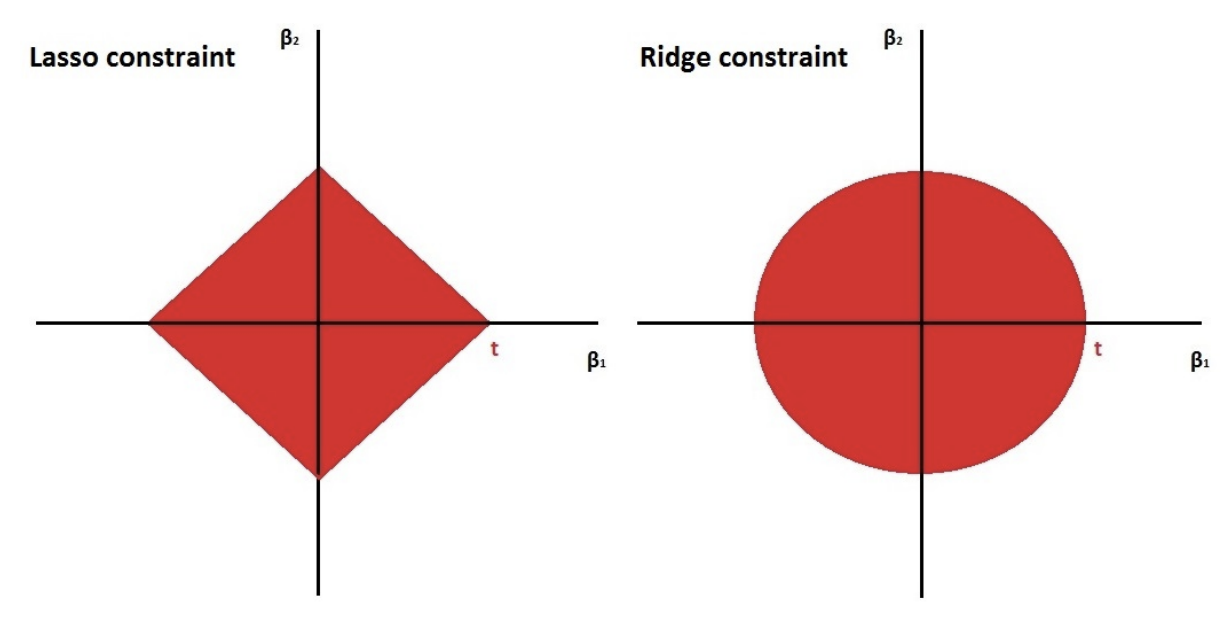
\includegraphics[width=0.55\textwidth]{Images/Ridge Lasso Geom.png}
    \caption{Left: the Lasso constraint \( |\beta_1| + |\beta_2| \leq c \),\quad Right: the Ridge constraint \( \beta_1^2 + \beta_2^2 \leq c \).}
    \label{fig:ridge-lasso-geom}
\end{figure}
\noindent In higher dimensions, so as $p$ increases, the \( \ell_2 \)-norm forms a hypersphere, which is a higher-dimensional generalisation of the circle. 

As the constraint region is circular, the ridge regression solution typically lies within the interior of the ball rather than on the axes. As a result, although ridge regression shrinks coefficients toward zero, it does not set any of them exactly to zero, even those corresponding to irrelevant predictors. 

This inability to create sparse models, i.e. a model in which some coefficients are exactly zero, is a key limitation of ridge regression, as it cannot perform feature selection. Ideally, a simpler model would exclude the uninformative variables entirely. Lasso regression does this.

\subsection{Lasso Regression}
\label{Lasso}
Lasso regression removes irrelevant features by shrinking their coefficients exactly to zero. Instead of penalising the squared magnitude of the coefficients like ridge, lasso penalises their absolute values. It shares the same aim of minimising a loss function as ridge, but with a different penalty term:
\begin{equation}
\mathcal{L}(\boldsymbol{\beta}) = \| \mathbf{Y} - \mathbf{X} \boldsymbol{\beta} \|_2^2 + \lambda \| \boldsymbol{\beta} \|_1,
\label{lasso-cost}
\end{equation}
\noindent or equivalently:
\[
\hat{\boldsymbol{\beta}}^{\text{Lasso}} = \arg\min_{\boldsymbol{\beta}} \left\{ \|\mathbf{Y} - \mathbf{X}\boldsymbol{\beta}\|_2^2 + \lambda \|\boldsymbol{\beta}\|_1 \right\},
\]
where $||\cdot||_1$ is the $\ell_1$-norm and the other variables follow from Equations~\ref{SRLR} and \ref{ridge-eqn}.

Unlike ridge regression, lasso has no closed-form solution because the \( \ell_1 \)-norm penalty, \( \| \boldsymbol{\beta} \|_1 \), is not differentiable at zero. This makes the optimisation problem non-smooth and means lasso requires iterative algorithms, such as coordinate descent, to solve it. 

\noindent Coordinate descent for the lasso regression, from Hastie et. al (2009),  proceeds as follows:

From SRLR, $\boldsymbol{\beta} \in \mathbb{R}^{p\times 1}$ and now suppose the \(p\) predictors and response are standardised to have mean zero and variance one. First, initialise all the \(\beta_j = 0\).

At each iteration, cycle over \(j = 1, \dots, p\) (the rows, or entries, of the coefficient vector) and update each coefficient by:

\begin{enumerate}
    \item First, computing the partial residual, $\mathbf{r}_j$, as:
\[
\mathbf{r}_j = \mathbf{Y} - \mathbf{X}_{-j} \boldsymbol{\beta}_{-j},
\]
where \(\mathbf{X}_{-j}\) denotes the design matrix, \(\mathbf{X}\), with the \(j\)-th column removed, and \(\boldsymbol{\beta}_{-j}\) is the coefficient vector, \(\boldsymbol{\beta}\), with the \(j\)-th entry removed.
\item Next, compute the simple least squares coefficient of these residuals on the $j$th predictor, $\beta_j^*$:
\[
\beta_j^* = \mathbf{x}_j^\top \mathbf{r}_j,
\]
where $\mathbf{x}_j$ is the $j$-th column of $\mathbf{X}$.
\item Finally, update \(\beta_j\) via soft-thresholding:
\[
\beta_j \leftarrow \text{sign}(\beta_j^*) \left( |\beta_j^*| - \lambda \right)_+,
\]
where \((z)_+ = \max(0, z)\) is the positive part function.\cite{hastie2008fast}
\end{enumerate}
\noindent This process repeats until convergence, which is defined as the point when the maximum change in the coefficient vector between successive iterations falls below a chosen threshold \(\epsilon_\text{Lasso} > 0\); that is, when:
\[
\|\boldsymbol{\beta}^{(k)} - \boldsymbol{\beta}^{(k-1)}\|_{\infty} < \epsilon_\text{Lasso},
\]
where \(\boldsymbol{\beta}^{(k)}\) denotes the coefficient vector after the \(k\)-th iteration, and \(\|\cdot\|_{\infty}\) is the maximum absolute value norm, where $\|\mathbf{x}\|_{\infty} = \max_{1 \leq i \leq n} |x_i|$.

Like ridge regression, lasso introduces bias in exchange for reduced variance, which can improve prediction accuracy. Lasso is particularly useful in high dimensions, as it is scalable and can perform automatic feature selection by shrinking some coefficients exactly to zero. Both ridge and lasso can also mitigate multicollinearity. However, for the equity fund dataset used in this report, such issues were largely addressed during preprocessing (see Chapter~\ref{EDA}).

As with ridge regression, this optimisation problem can be viewed as least squares subject to a different constraint, the $\ell_1$-norm:  $\| \boldsymbol{\beta} \|_1=\sum_{j=1}^p |\beta_j| \leq c$. Geometrically, in the two-dimensional case, when there are two predictors, this constraint defines a diamond-shaped region in the parameter space. The corners of this diamond lie on the coordinate axes, encouraging sparsity by increasing the chance that the solution lies exactly on one of them. This is why lasso can shrink some coefficients exactly to zero. See the left-hand graphic in Figure~\ref{fig:ridge-lasso-geom} for an illustration of this constraint.

In higher dimensions, the \( \ell_1 \)-norm forms a cross-polytope. This is a higher-dimensional generalisation of the diamond, which promotes sparsity by encouraging solutions closer to the axes.

These regularisation methods, developed for single-response models, can also be extended to MRR.

\subsection{Shrinkage Methods for MRR}
\label{SMs for MRR}
Ridge regression extends to MRR by adding a Frobenius norm penalty to the coefficient matrix, \(\mathbf{\hat{B}}^{\text{OLS}}\), from MRLR: 
\begin{equation}
\hat{\mathbf{B}}^\text{Ridge}=\arg\min_{\mathbf{B}}  \{\|\mathbf{Y} - \mathbf{XB}\|_F^2 + \lambda \|\mathbf{B}\|_F^2\},
    \label{multi-ridge-eqn}
\end{equation}
\noindent where $\lambda \geq 0$ is the regularisation parameter, \(\|\mathbf{B}\|_F^2 = \sum_{j=1}^{q} \sum_{i=1}^{m} b_{ij}^2\) denotes the Frobenius norm penalty, and the matrices $\mathbf{X}$, $\mathbf{Y}$ and $\mathbf{B}$ are defined as in Equation~\ref{MRLR}.\cite{mukherjee2011reduced}

In single-response ridge regression, the penalty is given by the squared \(\ell_2\)-norm of the coefficient vector. See Equation~\ref{ridge-eqn}. However, since the standard \(\ell_2\)-norm applies only to vectors, it cannot directly penalise all the entries in the coefficient matrix. The Frobenius norm replaces it because it extends the \(\ell_2\)-norm to matrices, summing the squared entries across all rows and columns in \(\mathbf{B}\).%, scaled by the regularisation parameter \(\lambda\).\cite{mukherjee2011reduced}

The closed-form solution for \(\mathbf{\hat{B}}^\text{Ridge}\) in multiple-response ridge regression is:

\begin{equation}
    \mathbf{\hat{B}}^\text{Ridge} = (\mathbf{X}^\top\mathbf{X} + \lambda \mathbf{I}_p)^{-1} \mathbf{X}^\top\mathbf{Y},
    \label{ridge}
\end{equation}

\noindent which follows from single-response ridge regression (see Equation~\ref{closed-form}).

Similarly, Lasso Regression can also be extended to MRR using the \(\ell_1\)-norm penalty: 
\begin{equation}
    \hat{\mathbf{B}}^\text{Lasso}=\arg\min_{\mathbf{B}} \{ \|\mathbf{Y} - \mathbf{XB}\|_F^2 + \lambda \|\mathbf{B}\|_1\}.
    \label{lasso mrr}
\end{equation}

\noindent As in single-response lasso regression, the \(\ell_1\)-penalty shrinks some elements of \(\mathbf{B}\) to exactly zero, enabling variable selection in the regression model.

Multivariate Lasso also uses coordinate descent to solve its optimisation problem. However, this slightly changes because now there is a coefficient matrix to estimate rather than a coefficient vector (see Subsection~\ref{multi-coord} for this algorithm).

Although Ridge and Lasso are MRR models as they build upon MRLR, they only consider the response covariance matrix through the joint estimation of the coefficient matrix. However, there are extensions of them that further exploit the multivariate response structure. Two such approaches are reduced rank ridge regression and multivariate regression with covariance estimation.

\subsection{Reduced Rank Ridge Regression}
In MRLR, predictions are generated using $\mathbf{Y}=\mathbf{X}\hat{\mathbf{B}}^{\text{OLS}}$ where $\mathbf{\hat{B}}^\text{OLS} = \mathbf{(X^\top X)}^{-1}\mathbf{X^\top Y}$.

Reduced rank ridge regression (RRRR) builds upon this by modifying the estimation of the coefficient matrix using multiple-response ridge regression (see Equation~\ref{multi-ridge-eqn}), and a rank constraint. It aims to solve the following optimisation problem:
\begin{equation}
\hat{\mathbf{B}}(\lambda, r) = \arg \min_{\mathbf{B}: \text{rank}(\mathbf{B}) \leq r} \|\mathbf{Y} - \mathbf{X} \mathbf{B}\|_F^2 + \lambda \|\mathbf{B}\|_F^2,
\label{RRRR OG}
\end{equation}
where $r\leq \text{min}$\{$p$, $m$\} controls the rank of $\mathbf{B}$ and $\lambda \geq 0$ is the ridge parameter. 

\noindent Note: $m$ is the number of responses and $p$ is the number of predictors.

Although the unconstrained ridge solution \(\hat{\mathbf{B}}^{\text{Ridge}}\) is typically full rank, which is confirmed on the equity fund dataset via QR-decomposition (see Subsection~\ref{Standard MRLR}), a rank constraint remains useful. It encourages dimensionality reduction and reflects the assumption that the responses are caused by a small number of latent variables.\cite{mukherjee2011reduced} This results in a model that not only considers the underlying latent structure of the data, but is also interpretable.

Before proceeding, assume that $\mathbf{X}$ and $\mathbf{Y}$ have been standardised, meaning each column has a mean of zero (mean-centring) and unit variance.
 As a result, the number of predictors, $p$, excludes the intercept term, and the column of ones is omitted from the design matrix. This assumption will be further justified later in this section.

The first step involves transforming Equation~\ref{RRRR OG} into a standard reduced rank regression problem
on an augmented dataset, which incorporates the ridge penalty.\cite{mukherjee2011reduced} This augmentation involves adding artificial rows to the original predictor and response matrices. 

The augmented least squares problem is equivalent to applying the closed-form ridge estimator from Equation~\ref{ridge}, when no rank constraint is applied. 
Augmentation is used instead in RRRR because it allows the RRRR problem to be solved more efficiently using Singular Value Decomposition (SVD), rather than solving the regularised optimisation problem directly.

Augmentation is also performed separately for each fixed \(\lambda\), as the optimal value is not known in advance and is selected via CV.

Here is augmentation written mathematically:
\begin{equation*}
    \mathbf{X}^*_{(n+p) \times p} = 
    \begin{pmatrix} 
        \mathbf{X} \\ 
        \sqrt{\lambda} \mathbf{I} 
    \end{pmatrix}, 
    \quad
    \mathbf{Y}^*_{(n+p) \times m} = 
    \begin{pmatrix} 
        \mathbf{Y} \\ 
        \mathbf{0} 
    \end{pmatrix}.
\end{equation*}

\noindent The augmented data leads to the following rank-constrained optimisation problem: 
\[\hat{\mathbf{B}}(\lambda, r) = 
\underset{\text{rank}(\mathbf{B}) \leq r}{\arg\min} 
\; \| \mathbf{Y}^* - \mathbf{X}^* \mathbf{B} \|_F^2,\]
%This solution is equivalent to an orthogonal projection onto the top $r$ singular vectors of the ridge-adjusted response matrix as established by the Eckhart–Young theorem. 
where $\mathbf{{B}}$ can be estimated using OLS. See Subsection~\ref{Mini Simp} for the full derivation of this.

This problem can be simplified further due to the orthogonality of the OLS estimate. This orthogonal projection property means the squared error loss function can be decomposed into 2 parts: 
\[\|\mathbf{Y}^* - \mathbf{X}^* \mathbf{B} \|_F^2 = \|\mathbf{Y}^* - \hat{\mathbf{Y}}^*_R \|_F^2 + \|\hat{\mathbf{Y}}^*_R - \mathbf{X}^* \mathbf{B} \|_F^2,\] 
where \( \hat{\mathbf{Y}}^*_R = \mathbf{X}^* \hat{\mathbf{B}}^*_R \) denotes the ridge regression estimate.\cite{mukherjee2011reduced} The first term of this equation does not involve $\mathbf{B}$ so the objective function can be further simplified into:
\begin{equation}
    \hat{\mathbf{B}}(\lambda, r) = \arg\min_{\operatorname{rank}(\mathbf{B}) \leq r} ||\hat{\mathbf{Y}}^*_R - \mathbf{X}^* \mathbf{B}||_{F}^2.
    \label{bhat}
\end{equation}

\noindent The next step involves decomposing the matrix \( \hat{\mathbf{Y}}^*_R\)
This starts by taking its SVD:
\[
    \hat{\mathbf{Y}}^*_R = \sum_{i=1}^{\tau} d_i \mathbf{u}_i \mathbf{v}_i^\top,
\]
where the \( d_i \)'s denote the singular values and \( \mathbf{u}_i \in \mathbb{R}^{n \times 1} \), \( \mathbf{v}_i \in \mathbb{R}^{m \times 1} \) denote the left and right singular vectors of \( \hat{\mathbf{Y}}^*_R \) respectively.\cite{mukherjee2011reduced} 

This step is important because RRRR further captures response intercorrelation through \( \mathbf{v}_i\). This can be proven by how the sample response covariance, $\mathbf{\hat{\Sigma}_Y}$, is defined:
\[
\mathbf{\hat{\Sigma}_Y}=\frac{1}{n-1}(\mathbf{Y}-\bar{\mathbf{Y}})^\top (\mathbf{Y}-\bar{\mathbf{Y}})=\frac{1}{n-1}\mathbf{Y}^\top\mathbf{Y}.
\]
The last equality holds because $\mathbf{Y}$ has been mean-centred
(see Subsection~\ref{SVD Cov} for how $\mathbf{\hat{\Sigma}_Y}$ and $\mathbf{Y}^\top\mathbf{Y}$ would relate without mean centring). 

This is important because the SVD of $\mathbf{Y}$ in matrix form is: $\mathbf{Y}=\mathbf{UDV}^\top$. Now, compute $\mathbf{Y^\top Y}$ using its SVD form:
\begin{equation*}
    \begin{aligned}
        \mathbf{Y^\top Y} &= \mathbf{VD^\top U^\top U DV^\top}\\ 
        &= \mathbf{VD}^2\mathbf{V^\top},
    \end{aligned}
\end{equation*}
\noindent where the final equality is produced because $\mathbf{U}$ is orthonormal, meaning $\mathbf{U^\top U}=\mathbf{I}_n$, and $\mathbf{D}=\mathbf{D^\top}$.\cite{jolliffe2002principal} This means $\mathbf{V}$ clearly diagonalises $\mathbf{Y^\top Y}$. Therefore, it directly represents the principal directions of response covariance. Thus, the columns of \( \mathbf{V} \), \( \mathbf{v}_i\), capture response intercorrelation.

Then, the Eckhart-Young Theorem is used to provide the best rank \( r \) approximation to \( \hat{\mathbf{Y}}^*_R \) in the Frobenius norm as follows:
\[
\hat{\mathbf{Y}}^*_r = \sum_{i=1}^{r} d_i \mathbf{u}_i \mathbf{v}_i^\top.\cite{mukherjee2011reduced}
\]

The next step to RRRR is to define the projection matrix, $\mathbf{P}_r$, which projects the predictions onto an $r$-dimensional subspace: \( \mathbf{P}_r = \sum_{i=1}^{r} \mathbf{v}_i \mathbf{v}_i^\top \).

Let \( \hat{\mathbf{B}}(\lambda, r) = \hat{\mathbf{B}}^*_R \mathbf{P}_r \) and  clearly, \(\operatorname{rank}(\hat{\mathbf{B}}(\lambda, r)) \leq r\), as \(\operatorname{rank}(\mathbf{P}_r) = r\).\cite{mukherjee2011reduced} Substituting this into the fitted values, $\mathbf{X}^* \hat{\mathbf{B}}(\lambda, r)$, we obtain predictions corresponding to the rank-$r$ solution in Equation~\ref{bhat}, and thereby to the original problem in Equation~\ref{RRRR OG}:
\[
\mathbf{X}^* \hat{\mathbf{B}}(\lambda, r) = \mathbf{X}^* \hat{\mathbf{B}}^*_R \mathbf{P}_r
= \left( \sum_{i=1}^{\tau} d_i \mathbf{u}_i \mathbf{v}_i^\top \right)
\left( \sum_{j=1}^{r} \mathbf{v}_j \mathbf{v}_j^\top \right)
= \sum_{i=1}^{r} d_i \mathbf{u}_i \mathbf{v}_i^\top = \hat{\mathbf{Y}}^*_r.\cite{mukherjee2011reduced}
\]
See Subsection~\ref{proj} for the third simplification.

This has shown that the proposed solution \( \hat{\mathbf{B}}(\lambda, r) = \hat{\mathbf{B}}^*_R \mathbf{P}_r \) is the minimiser of Equation~\ref{bhat} and hence the optimisation problem.\cite{mukherjee2011reduced} Writing it explicitly in terms of \( \mathbf{X}, \mathbf{Y}, \lambda \) and \( r \) gives the following:
\[
\hat{\mathbf{B}}(\lambda, r) = \hat{\mathbf{B}}^*_R \mathbf{P}_r = (\mathbf{X}^{*\top} \mathbf{X}^*)^{-1} \mathbf{X}^{*\top} \mathbf{Y} \mathbf{P}_r
= (\mathbf{X}^\top \mathbf{X} + \lambda \mathbf{I})^{-1} \mathbf{X}^\top \mathbf{Y} \mathbf{P}_r.\cite{mukherjee2011reduced}
\]
Therefore:
\(\hat{\mathbf{Y}}(\lambda, r) = \mathbf{X}\hat{\mathbf{B}}(\lambda, r) =\mathbf{X}\hat{\mathbf{B}}^*_R \mathbf{P}_r= \mathbf{X} \left( \mathbf{X}^\top \mathbf{X} + \lambda \mathbf{I} \right)^{-1} \mathbf{X}^\top \mathbf{Y} \mathbf{P}_r = {\mathbf{X}}\hat{\mathbf{B}}^\text{Ridge} \mathbf{P}_r.\)

From this estimate, the role of the ridge closed-form solution becomes clear: the full-rank ridge estimator $\hat{\mathbf{B}}^*_R$ is first computed, and then its fitted values $\hat{\mathbf{Y}}_\lambda = \mathbf{X}^* \hat{\mathbf{B}}^*_R$ are projected onto a lower-dimensional subspace. The rank-$r$ constraint then arises from this projection, which maps the fitted values from the original $m$-dimensional response space to an $r$-dimensional subspace spanned by the top $r$ right singular vectors.

While RRRR further accounts for response covariance by applying SVD to a low-rank approximation of the fitted response matrix, an alternative approach is to model the inverse error covariance matrix, which captures conditional dependencies between responses directly. This idea underlies Multivariate Regression with Covariance Estimation, which jointly estimates both the coefficient and inverse error covariance matrices.

\subsection{Multivariate Regression with Covariance Estimation}
Multivariate Regression with Covariance Estimation (MRCE) builds upon MRLR by jointly estimating the regression coefficient matrix \( \mathbf{B} \) and the inverse error covariance matrix \( \mathbf{\Omega} = \mathbf{\Sigma}^{-1}_\mathbf{E} \).

\noindent Before solving this problem, we again assume that $\mathbf{X}$ and $\mathbf{Y}$ have been standardised. 

Starting with the familiar MRLR model:
\[
\mathbf{Y}_{(n\times m)} = \mathbf{X}_{(n \times p)} \mathbf{B}_{(p \times m)} + \mathbf{E}_{(n \times m)},
\]
where $p$ no longer includes the column of ones.

Each row \( \mathbf{y}_i \in \mathbb{R}^{1 \times m} \) of \( \mathbf{Y} \) follows the conditional distribution:
\[\mathbf{y}_i|\mathbf{x}_i \sim \mathcal{N}_m(\mathbf{x}_i \mathbf{B}, \mathbf{\Sigma_E})\] 
from the multivariate normality of the errors. Therefore, the probability density function for the $i^{th}$ row, i.e. a single observation, is:
\begin{equation}
p(\mathbf{y}_i \mid \mathbf{x}_i) = \frac{1}{(2\pi)^{m/2} |\mathbf{\Sigma_E}|^{1/2}} \exp\left( -\frac{1}{2} (\mathbf{y}_i - \mathbf{x}_i \mathbf{B})^\top \mathbf{\Sigma}^{-1}_\mathbf{E} (\mathbf{y}_i - \mathbf{x}_i \mathbf{B}) \right).
\label{pdf}
\end{equation}

\noindent Equation~\ref{pdf} implies that, in MRLR, the negative log-likelihood function of \( (\mathbf{B}, \mathbf{\Omega}) \) can be expressed up to a constant as:
\begin{equation*}
    g(\mathbf{B}, \boldsymbol{\Omega}) = \text{tr} \left[ \frac{1}{n} (\mathbf{Y} - \mathbf{X} \mathbf{B})^\top (\mathbf{Y} - \mathbf{X} \mathbf{B}) \boldsymbol{\Omega} \right] - \log |\boldsymbol{\Omega}|.\cite{rothman2010sparse}
\end{equation*}
See Subsection~\ref{NLL} for the full derivation.

The MRCE estimation for $\mathbf{B}$ extends this by adding 2 penalties to the negative log-likelihood function, $g$, to construct a sparse estimator of $\mathbf{B}$ depending on $\mathbf{\Omega}$:
\begin{equation}
    (\hat{\mathbf{B}}, \hat{\boldsymbol{\Omega}}) = \arg \min_{\mathbf{B}, \boldsymbol{\Omega}} \left\{ g(\mathbf{B}, \boldsymbol{\Omega}) + \lambda_1 \sum_{j' \neq j} |\omega_{j'j}| + \lambda_2 \sum_{j=1}^{p} \sum_{k=1}^{q} |b_{jk}| \right\},
    \label{MRCE}
\end{equation}
\noindent where \( \omega_{j'j} \) are the elements of \( \boldsymbol{\Omega} \), \( b_{jk} \) are the elements of \( \mathbf{B} \), \( \lambda_1 \) controls sparsity in \( \boldsymbol{\Omega} \) and \( \lambda_2 \) for \( \mathbf{B} \).\cite{rothman2010sparse} 

\noindent Equation~\ref{MRCE} can be solved in 2 ways: by solving it for \( \mathbf{\hat{B}} \) with \( \mathbf{\Omega} \) fixed at a chosen \( \mathbf{\Omega}_0 \) and by solving for \( \mathbf{\hat{\Omega}} \) with \( \mathbf{B} \) fixed at a chosen \( \mathbf{B}_0 \):

\begin{enumerate}
    \item This is the formula for \( \mathbf{\hat{B}} \), fixing \( \boldsymbol{\hat{\Omega}} \) as \( \boldsymbol{\Omega}_0 \), therefore the $\mathbf{\Omega}$ terms in Equation~\ref{MRCE} can be removed from the objective function:
        \begin{equation}
            \hat{\mathbf{B}}(\boldsymbol{\Omega}_0) = \arg \min_{\mathbf{B}} \left\{ \text{tr} \left[ \frac{1}{n} (\mathbf{Y} - \mathbf{X} \mathbf{B})^\top (\mathbf{Y} - \mathbf{X} \mathbf{B}) \boldsymbol{\Omega}_0 \right]+ \lambda_2 \sum_{j,k} |b_{jk}| \right\}.
        \label{B as Omega}
        \end{equation}
    \item This is the formula for \( \boldsymbol{\Omega} \), fixing \( \mathbf{B} \) as \( \mathbf{B}_0 \), therefore the $\mathbf{B}$ terms in Equation~\ref{MRCE} can be removed from the objective function:
        \begin{equation}
            \hat{\boldsymbol{\Omega}}(\mathbf{B}_0) = \arg \min_{\boldsymbol{\Omega}} \left\{ \text{tr} \left[ \hat{\mathbf{\Sigma}}_R \boldsymbol{\Omega} \right] - \log |\boldsymbol{\Omega}| + \lambda_1 \sum_{j' \neq j} |\omega_{j'j}| \right\}.
        \label{Omega as B}
        \end{equation}
\end{enumerate}
\noindent where $\hat{\mathbf{\Sigma}}_R=\frac{1}{n} (\mathbf{Y} - \mathbf{X} \mathbf{B}_0)^\top (\mathbf{Y} - \mathbf{X} \mathbf{B}_0)$.

Before delving further into this problem, let us discuss how this model qualifies as MRR and, consequently, how it accounts for response intercorrelation. 

Since MRCE estimates both \( \mathbf{B} \) and \( \mathbf{\Omega} \) simultaneously, the coefficient matrix is optimised considering response covariance. This reasoning follows from the explanation for why MRLR qualifies as an MRR (see Equation~\ref{MRLR = MRR} for this).

The error covariance matrix, \( \mathbf{\Sigma_E} \), describes marginal dependencies between response variables, whereas the inverse error covariance matrix, \( \mathbf{\Omega} = \mathbf{\Sigma}^{-1}_\mathbf{E} \), describes conditional dependencies.\cite{10.1093/biomet/asq060} This means that if \( \Omega_{ij} = 0 \), then responses \( Y_i \) and \( Y_j \) are conditionally independent given all other responses and, if \( \Omega_{ij} \neq 0 \), then responses \( Y_i \) and \( Y_j \) have a dependency not accounted for by the predictors.\cite{10.1093/biomet/asq060}
Thus, MRCE does not assume independent residuals, but instead models how responses are related even after accounting for predictors. 
By contrast, MRLR assumes that \( \mathbf{\Sigma_E} \) is unstructured but fixed during estimation, and does not account for conditional error dependencies when estimating \( \mathbf{B} \).

Equations~\ref{B as Omega} and \ref{Omega as B} are each solved using a distinct approach. Equation~\ref{B as Omega} is solved by the following algorithm. Let us call it Algorithm 1. This algorithm comes from Friedman et al. (2007):

\noindent Given \( \mathbf{\Omega} \) and an initial value \( \hat{\mathbf{B}}^{(0)} \), let \( \mathbf{S} = \mathbf{X}^\top \mathbf{X} \) and \( \mathbf{H} = \mathbf{X}^\top \mathbf{Y} \mathbf{\Omega} \), the algorithm goes as follows:

\begin{enumerate}

\item  For the \( t \)-th iteration, set \( \hat{\mathbf{B}}^{(t)} \leftarrow \hat{\mathbf{B}}^{(t-1)} \). Visit all entries of \( \hat{\mathbf{B}}^{(m)} \) in some sequence, and for each entry \( (r, c) \), update \( \hat{b}^{(t)}_{rc} \) by minimising the objective function with respect to that single entry, keeping all other coefficients fixed:
\[
\hat{b}^{(t)}_{rc} \leftarrow \operatorname{sign} \left( \hat{b}^{(t)}_{rc} + \frac{h_{rc} - u_{rc}}{s_{rr} \omega_{cc}} \right) 
\left( \left| \hat{b}^{(t)}_{rc} + \frac{h_{rc} - u_{rc}}{s_{rr} \omega_{cc}} \right| - \frac{n \lambda_2}{s_{rr} \omega_{cc}} \right)_{+},
\]
where $u_{rc} = \sum_{j=1}^{p} \sum_{k=1}^{q} \hat{b}^{(t)}_{jk} s_{rj} \omega_{kc}$ and $(a)_+$ means taking max$(a,0)$. 

\item If $\sum_{j,k} \left| \hat{b}^{(t)}_{jk} - \hat{b}^{(t-1)}_{jk} \right| < \epsilon_\text{Ridge} \sum_{j,k} \left| \hat{b}^{\text{Ridge}}_{jk} \right|$,
then stop, otherwise go to the prior step. Here: $\hat{\mathbf{B}}^{\text{Ridge}}$ is the ridge closed-form estimator of the coefficient matrix (see Equation~\ref{ridge} for this estimator).
\end{enumerate}
\noindent For the full derivation of Algorithm 1, see Subsection~\ref{alg 1}.

%\noindent Note: \( \epsilon \) specifies how small the change in \( \hat{\mathbf{B}} \) must be between iterations for the algorithm to be considered converged.

Equation~\ref{Omega as B} is solved using the graphical lasso (see Subsection~\ref{glasso} for further justification). It is solved using this algorithm due to its speed.\cite{rothman2010sparse} Graphical lasso (glasso) is widely used for estimating sparse inverse covariance matrices in high-dimensional cases. Its algorithm, from Banerjee et al. (2007) and Friedman et al. (2008), is as follows:
\begin{enumerate}
    \item First, define \( \boldsymbol{\hat{\Omega}}^{(t+1)}_{0} = (\mathbf{S} + \lambda_1 \mathbf{I}_m)^{-1} \), where $\boldsymbol{\hat{\Omega}}^{(t+1)}_{0}$ denotes the initial iteration of $\boldsymbol{\hat{\Omega}}^{(t+1)}$ and \( \mathbf{S} = \hat{\boldsymbol{\Sigma}}_R = \frac{1}{n} (\mathbf{Y} - \mathbf{X} \mathbf{\hat{B}}^{({t+1})})^\top (\mathbf{Y} - \mathbf{X} \mathbf{\hat{B}}^{({t+1})}) \) is the empirical error covariance matrix computed at fixed \( \mathbf{\hat{B}}^{({t+1})} \). 
    
    %Note: the diagonal of \( \mathbf{\Omega} \) remains unchanged in what follows.
    
    \item For the $i$-th intermediate update of $\mathbf{\hat{\Omega}}^{(t+1)}$, $\mathbf{\hat{\Omega}}^{(t+1)}_i$, (this update comes from co-ordinate descent, whose relevance will be explained later, on each column of $\mathbf{\hat{\Omega}}^{(t+1)}_i$) and each column: \( j = 1, 2, \dots, m\), {solve for the \( j \)-th column of $\mathbf{\hat{\Omega}}^{(t+1)}_i$}, {while keeping the rest of $\mathbf{\hat{\Omega}}^{(t+1)}_i$ fixed}. Let us denote $\mathbf{\hat{\Omega}}^{(t+1)}_i$ as $\mathbf{\Omega}$ in this step for brevity.

%Note: carrying this update out for all columns gives the next iteration, \( \hat{\boldsymbol{\Omega}}^{(t+1)}_{i+1} \).
%For each column \( j = 1, 2, \dots, m \), solve for the \( j \)-th column of \( \widehat{\boldsymbol{\Omega}}^{(t+1)} \) using coordinate descent. Let \( i \) index the intermediate updates within the Lasso problem for column \( j \), and write \( \hat{\boldsymbol{\Omega}}^{(t+1)}_i \) to denote the matrix after the \( i \)-th coordinate update. We denote this as \( \boldsymbol{\Omega} \) for brevity in the steps below.


    %\begin{enumerate}
        First, partition both \( \mathbf{\Omega} \) and \( \mathbf{S} \) as:
  \[
  \mathbf{\Omega} = \begin{bmatrix}
    \mathbf{\Omega}_{-j,-j} & \boldsymbol{\omega}_{-j,j} \\
    \boldsymbol{\omega}_{j,-j} & \omega_{jj}
  \end{bmatrix},
  \quad
  \mathbf{S} = \begin{bmatrix}
    \mathbf{S}_{-j,-j} & \mathbf{s}_{-j,j} \\
    \mathbf{s}_{j,-j} & s_{jj}
  \end{bmatrix},
  \]
  where \( \mathbf{\Omega}_{-j,-j} \) is \( \mathbf{\Omega} \) with the \( j \)-th row and column removed, and \( \boldsymbol{\omega}_{-j,j} \) is the \( j \)-th column of $\mathbf{\Omega}$ excluding the diagonal entry \( \omega_{jj} \) (and likewise logic for $\mathbf{S}$).

  \noindent Note: Since \( \boldsymbol{\Omega} \) and \( \mathbf{S} \) are symmetric, updating the \( j \)-th column determines the \( j \)-th row.

%Banerjee et al. (2007) show the solution for $\boldsymbol{\omega}_{-j,j}$ satisfies:
%\begin{equation}
%\boldsymbol{\omega}_{-j,j} = %\arg\min_{\mathbf{y}} \left\{ \mathbf{y}^\top %\mathbf{\Omega}_{-j,j}^{-1} \mathbf{y} \,:\, %\|\mathbf{y} - \mathbf{s}_{-j,j}\|_\infty %\leq \lambda_1 \right\}.
%\label{primal}
%\end{equation}
  
   Now, define:
  \[
  \mathbf{P} = \mathbf{\Omega}^{1/2}_{-j,-j}, \quad \mathbf{b} = \mathbf{\Omega}_{-j,-j}^{-1/2}\mathbf{s}_{-j,j}.
  \]
  Here, $\boldsymbol{\Omega}_{-j,-j}^{1/2}$ refers to the unique symmetric positive definite matrix such that:
\[
\boldsymbol{\Omega}_{-j,-j}^{1/2} \, \boldsymbol{\Omega}_{-j,-j}^{1/2} = \boldsymbol{\Omega}_{-j,-j},
\]
and likewise for $\boldsymbol{\Omega}_{-j,-j}^{-1/2}$:
\[
\boldsymbol{\Omega}_{-j,-j}^{-1/2} \, \boldsymbol{\Omega}_{-j,-j}^{-1/2} = \boldsymbol{\Omega}^{-1}_{-j,-j}.
\]
These matrices are obtained via eigen-decomposition.

Banerjee et al. (2007) showed that solving the problem for $\boldsymbol{\omega}_{-j,j}$ is equivalent to solving
the following dual problem for \( \boldsymbol{\beta} \), where $\boldsymbol{\beta} \in \mathbb{R}^{m-1}$ is an intermediate vector:
  \[
\min_{\boldsymbol{\beta}} \left\{ \| \mathbf{b} - \mathbf{P} \boldsymbol{\beta} \|_2^2 + \lambda_1 \| \boldsymbol{\beta} \|_1 \right\}.
\]
This is the lasso problem, where \( \mathbf{P}\boldsymbol{\beta} \) is the prediction and \( \mathbf{b} \) is the pseudo-response. Therefore, it can be solved by coordinate descent (see Subsection~\ref {Lasso}).

\vspace{0.1cm}
This gives a \( m - 1 \) vector solution \( \hat{\boldsymbol{\beta}} \). 
    Finally, fill in the corresponding column (and hence row) of \( \mathbf{\Omega} \) using 
    \( \boldsymbol{\omega}_{-j,j} = \mathbf{\Omega}_{-j,-j}\hat{\boldsymbol{\beta}}\). This update only adjusts the off-diagonal elements of $\mathbf{\Omega}$ as these directly relate to the dependencies between responses.
    
\item Once all \( m \) columns (and hence rows) have been updated by coordinate descent, this gives the matrix \( \hat{\boldsymbol{\Omega}}^{(t+1)}_{i+1} \) for the next iteration. Step 2 is repeated until convergence between successive iterations, which is when for some $k+1$-th iteration:
\[
\|\boldsymbol{\hat{\Omega}}^{(t+1)}_{k+1} - \boldsymbol{\hat{\Omega}}^{(t+1)}_{k}\|_{\infty} < \epsilon_\text{Omega},\
\]
where $\epsilon_\text{Omega}$ is the convergence threshold for the inverse error covariance matrix.\cite{friedman2008sparse, banerjee2008model}

Therefore, when this convergence occurs, $\mathbf{\hat{\Omega}}^{(t+1)}=\boldsymbol{\hat{\Omega}}^{(t+1)}_{k+1}$.
\end{enumerate}
\noindent Now, we can explicitly outline the full MRCE algorithm from Rothman et al. (2010) as follows:

\vspace{0.1cm}
\noindent For fixed values of \( \lambda_1 \) and \( \lambda_2 \), initialise \( \hat{\mathbf{B}}^{(0)} = \mathbf{0} \) and \( \hat{\mathbf{\Omega}}^{(0)} = \hat{\mathbf{\Omega}}(\hat{\mathbf{B}}^{(0)}) \). 
\begin{enumerate}
    \item Compute \( \hat{\mathbf{B}}^{(t+1)} = \hat{\mathbf{B}}(\hat{\mathbf{\Omega}}^{(t)}) \) by solving Equation~\ref{B as Omega} using Algorithm 1.

    \item Compute \( \hat{\mathbf{\Omega}}^{(t+1)} = \hat{\mathbf{\Omega}}(\hat{\mathbf{B}}^{(t+1)}) \) by solving Equation~\ref{Omega as B} using the glasso algorithm.

    \item If $\sum_{j,k} \left| \hat{b}^{(t+1)}_{jk} - \hat{b}^{(t)}_{jk} \right| < \epsilon_\text{Ridge} \sum_{j,k} \left| \hat{b}^{\text{Ridge}}_{jk} \right|$,
then stop; otherwise, go back to Step 1.
\end{enumerate}

\noindent Therefore, when updating $\mathbf{\Omega}$ only the dependencies between responses are updated which means $\mathbf{\hat{B}}$ is updated considering this.

%This process uses blockwise descent to compute a local solution for Equation~\ref{MRCE} with steps 1 and 2 decreasing the objective function value.\cite{rothman2010sparse}

MRCE performance also depends on the regularisation parameters, which are selected via CV:
\begin{equation*}
    (\lambda_1^*, \lambda_2^*) = \arg \min_{\lambda_1, \lambda_2} \sum_{k=1}^{K} \| \mathbf{Y}^{(k)} - \mathbf{X}^{(k)} \mathbf{B}_{\lambda_1, \lambda_2}^{(-k)} \|_F^2,
\end{equation*}
where \( \mathbf{Y}^{(k)} \) is the matrix of responses with observations in the \( k \)th fold, \( \mathbf{X}^{(k)} \) is the matrix of predictors of observations in the \( k \)th fold, and \( \mathbf{B}_{\lambda_1, \lambda_2}^{(-k)} \) is the estimated regression coefficient matrix computed with observations outside the \( k \)th fold, 
with tuning parameters \( \lambda_1 \) and \( \lambda_2 \).\cite{rothman2010sparse} 

\noindent The next section will talk about how these 2 methods were evaluated on the equity fund dataset.

\vspace{-0.2cm}
\section{Application}
Although standardisation involves both mean-centring and scaling to unit variance for $\mathbf{X}$ and $\mathbf{Y}$, only mean-centring is shown in these calculations for brevity.
\vspace{-0.2cm}
\subsection{Small-Scale Example}
Let us now apply both of these shrinkage methods to a small dataset before proceeding to the equity fund dataset. We will use the familiar Mathematics and Science scores data:

% Adjust column spacing
\begin{table}[H]
    \centering
    \begin{tabular}{|c|c|c|c|}
        \hline
        \( X_1 \): Hours Studied & \( X_2 \): Time Spent on Papers & \( Y_1 \): Math Scores & \( Y_2 \): Science Scores\\
        \hline
        5  & 2  & 78 & 80 \\
        7  & 3  & 85 & 79 \\
        8  & 4  & 88 & 88 \\
        3  & 1  & 65 & 70 \\
        10 & 5  & 92 & 74 \\
        \hline
    \end{tabular}
    \caption{Study Time vs. Exam Scores}
    \label{tab:study_scores4}
\end{table}
\subsubsection{Reduced Rank Ridge Regression}
This example will show a rank-1 reduction of RRRR using $\lambda = 0.1$ as the shrinkage parameter.

Based on our prior justification of RRRR as an MRR model, mean-centring is essential to prevent biasing from the mean structure. The initial predictor matrix, \( \mathbf{X} \), and initial response matrix, \( \mathbf{Y} \), are:

\[
\mathbf{X} = 
\begin{bmatrix}
5 & 7 & 8 & 3 & 10 \\
2 & 3 & 4 & 1 & 5
\end{bmatrix}^\top, 
\quad
\mathbf{Y} = 
\begin{bmatrix}
78 & 85 & 88 & 65 & 92 \\
80 & 79 & 88 & 70 & 74
\end{bmatrix}^\top.
\]
\noindent After mean-centering, i.e. $\mathbf{\tilde{X}} = \mathbf{X}-\mathbf{\bar{X}}$ and $\mathbf{\tilde{Y}} = \mathbf{Y}-\mathbf{\bar{Y}}$, the predictor and response matrices become:

\[
\tilde{\mathbf{X}} =
\begin{bmatrix}
-1.6  & 0.4  & 1.4  & -3.6  & 3.4 \\
-1  & 0  & 1  & -2  & 2
\end{bmatrix}^{\top},
\quad
\tilde{\mathbf{Y}} =
\begin{bmatrix}
-3.6  & 3.4  & 6.4  & -16.6  & 10.4 \\
1.8  & 0.8  & 9.8  & -8.2  & -4.2
\end{bmatrix}^{\top}.
\]

\noindent We apply RRRR with \( \lambda = 0.01 \) by first incorporating ridge regularisation, which we define as:
\[
\mathbf{X}^* =
\begin{bmatrix}
\mathbf{\tilde{X}} \\
\sqrt{\lambda} \mathbf{I}
\end{bmatrix}
, \quad
\mathbf{Y}^* =
\begin{bmatrix}
\mathbf{\tilde{Y}} \\
\mathbf{0}
\end{bmatrix}.
\]
Since \( \lambda = 0.01 \), we compute \( \sqrt{\lambda} = \sqrt{0.01} = 0.1 \), so the augmented matrices are:
\[
\mathbf{X}^* =
\begin{bmatrix}
-1.6  & 0.4  & 1.4  & -3.6  & 3.4 & 0.1 & 0\\
-1  & 0  & 1  & -2  & 2 & 0 & 0.1
\end{bmatrix}^{\top},
\quad
\mathbf{Y}^* =
\begin{bmatrix}
-3.6  & 3.4  & 6.4  & -16.6  & 10.4 & 0 & 0 \\
1.8  & 0.8  & 9.8  & -8.2  & -4.2 & 0 & 0
\end{bmatrix}^{\top}.
\]
The Ridge penalty is incorporated into \( \mathbf{X}^* \) through \( \sqrt{\lambda} \mathbf{I} \).
The augmented system behaves like a standard regression problem, meaning we solve for \( \mathbf{B} \) using the standard OLS formula. Let us denote this as $\hat{\mathbf{B}}^*_R$ as a reminder that we are incorporating ridge regression.

\noindent Using the OLS estimate formula: $\hat{\mathbf{B}}^*_R = (\mathbf{X}^{*\top} \mathbf{X}^*)^{-1} \mathbf{X}^{*\top} \mathbf{Y}^*$. After subbing in $\mathbf{X}^*$ and $\mathbf{Y}^*$, this gives us the augmented coefficient matrix, $\hat{\mathbf{B}}^*_R$:
\[
\hat{\mathbf{B}}^*_R =
\begin{bmatrix}
7.40 & -2.28 \\
-6.18 & 5.47
\end{bmatrix}.
\]
\vspace{-0.3cm}
Thus, the ridge predictions are:
\[
\hat{\mathbf{Y}}^*_R =
\mathbf{X}^* \hat{\mathbf{B}}^*_R
=
\begin{bmatrix}
-5.67 & 2.96 & 4.19 & -14.29 & 12.81 & 0.74 & -0.62 \\
-1.82 & -0.91 & 2.28 & -2.73 & 3.19 & -0.23 & 0.55
\end{bmatrix}^{\top}.
\]
The next step is to perform SVD on this prediction, i.e. $\hat{\mathbf{Y}}^*_R = \mathbf{U} \mathbf{D} \mathbf{V}^\top$. This gives (to 3sf):
\[
\mathbf{D} =
\begin{bmatrix}
21.209 & 0 \\
0 & 2.294
\end{bmatrix}, \quad
\mathbf{V} =
\begin{bmatrix}
0.975 & -0.223 \\
0.223 & 0.975
\end{bmatrix} \quad \text{and}
\]
\[
\mathbf{U} =
\begin{bmatrix}
-0.280 & 0.127 & 0.216 & -0.686 & 0.622 & 0.0316 & -0.0227 \\
-0.224 & -0.675 & 0.562 & 0.227 & 0.111 & -0.169 & 0.293
\end{bmatrix}^{\top}.
\]
For full derivation of $\mathbf{D}, \mathbf{U}$ and $\mathbf{V}$ see Subsection~\ref{RRR SVD}. 

Since \( D_1 = 21.21 \gg D_2 = 2.29 \), the best rank ($r$=1) approximation is taken on the first column of $\mathbf{D}$. Therefore, $\hat{\mathbf{Y}}^*_1 \approx d_1 \mathbf{u}_1 \mathbf{v}_1^\top,$
where (to 3sf):
\[
d_1 = 21.209, \quad 
\mathbf{v}_1 =
\begin{bmatrix}
0.975 & 0.223
\end{bmatrix}^\top \quad \text{and}
\]
\vspace{-0.3cm}
\[
\mathbf{u}_1 =
\begin{bmatrix}
-0.280 & 0.127 & 0.216 & -0.686 & 0.622 & 0.0316 & -0.0227
\end{bmatrix}^\top.
\]
However, this is just an intermediary step as we still need to rescale the coefficient matrix. This is done through the projection matrix, $\mathbf{P}_r$:
\[
\mathbf{P}_r =\mathbf{v}_1 \mathbf{v}_1^\top
 =
\begin{bmatrix}
0.95 & 0.22 \\
0.22 & 0.05
\end{bmatrix}.
\]
Finally, the RRRR estimator is:
\vspace{-0.3cm}
\[
\hat{\mathbf{B}}_r=
 \hat{\mathbf{B}}^*_R \mathbf{P}_r
 =
\begin{bmatrix}
6.54 & 1.49 \\
-4.68 & -1.07
\end{bmatrix}.
\]
Now, we can do the final predicted values, which are $\mathbf{\hat{Y}}=\mathbf{\tilde{X}^*\hat{B}}_r$, giving:
\[
\mathbf{\hat{Y}}=
\begin{bmatrix}
-5.78 & 2.62 & 4.47 & -14.18 & 12.87 \\
-1.32 & 0.60 & 1.02 & -3.24 & 2.94
\end{bmatrix}^{\top}.
\]
Remember, these predictions are on the mean-centred $\mathbf{Y}$.
We can remove this mean-centring, but that does not affect its model fit evaluation using the ANRMSE as these predictions can just be compared to the actual mean-centred $\mathbf{Y}$.
\vspace{-0.3cm}
\subsubsection{Multivariate Regression with Covariance Estimation}
Now, we perform an MRCE iteration on Table~\ref{tab:study_scores4} with \(\lambda_1 = \lambda_2 = 0.1\). Remember we want to mean centre $\mathbf{X}$ and $\mathbf{Y}$, so let us use \(\mathbf{\tilde{X}}\) and \(\mathbf{\tilde{Y}}\) from the RRRR calculation: 
\[
\tilde{\mathbf{X}} =
\begin{bmatrix}
-1.6  & 0.4  & 1.4  & -3.6  & 3.4 \\
-1  & 0  & 1  & -2  & 2
\end{bmatrix}^{\top},
\quad
\tilde{\mathbf{Y}} =
\begin{bmatrix}
-3.6  & 3.4  & 6.4  & -16.6  & 10.4 \\
1.8  & 0.8  & 9.8  & -8.2  & -4.2
\end{bmatrix}^{\top}.
\]
From here on, $\mathbf{X} = \tilde{\mathbf{X}}$ and $\mathbf{Y} = \tilde{\mathbf{Y}}$. This is to make notation easier. Let us first compute $\mathbf{\hat{B}}^{\text{Ridge}}$ because that is used in determining when Algorithm 1 stops:
%\vspace{-0.2cm}
\[
\mathbf{\hat{B}}^{\text{Ridge}}=(\mathbf{X}^\top \mathbf{X} + \lambda_2 \mathbf{I})^{-1} \mathbf{X}^\top \mathbf{Y}=\begin{bmatrix}
5.07  & -0.77  \\
-2.19  & 2.89 
\end{bmatrix}.
\]
For Algorithm 1, initialise \(\hat{\mathbf{B}}^{(0)} = \mathbf{0} \) and \( \hat{\mathbf{\Omega}}^{(0)} = \hat{\mathbf{\Omega}}(\hat{\mathbf{B}}^{(0)}) \).
To compute $\hat{\mathbf{\Omega}}^{(0)}$, first do the error, $\mathbf{E}^{(0)}$:
%\vspace{-0.2cm}
\[
\mathbf{\mathbf{E}}^{(0)} = \mathbf{Y} - \mathbf{X} \mathbf{\hat{B}}^{(0)} =
\begin{bmatrix}
-3.6  & 3.4  & 6.4  & -16.6  & 10.4 \\
1.8  & 0.8  & 9.8  & -8.2  & -4.2
\end{bmatrix}^{\top}.
\]
Now, compute the residual covariance matrix \(\ \mathbf{\Sigma}^{(0)}_\mathbf{E}\):
%\vspace{-0.2cm}
\[
\mathbf{\Sigma}^{(0)}_\mathbf{E}= \frac{1}{n} \mathbf{\mathbf{E}}^{{(0)^{\top}}} \mathbf{\mathbf{E}}^{(0)} =
\begin{bmatrix}
89.84 & 30.28 \\
30.28 & 36.96
\end{bmatrix}.
\]
Next, add this to a regularisation parameter, $\lambda_2=0.1$, and invert. The regularisation parameter avoids dividing by zero when inverting $\mathbf{\Sigma_E}^{(0)}$ for the precision matrix (to 3dp):
\begin{equation}
\mathbf{\Omega}^{(0)} = (\mathbf{\Sigma}^{(0)}_\mathbf{E} + \lambda_2 \mathbf{I}_m)^{-1} = \begin{bmatrix}
0.015 & -0.013 \\
-0.013 & 0.037
\end{bmatrix}.
\end{equation}

\noindent Now compute \( \hat{\mathbf{B}}^{(1)} = \hat{\mathbf{B}}(\hat{\mathbf{\Omega}}^{(0)}) \) by solving Equation~\ref{B as Omega} using Algorithm 1. The manual calculation of this will be shown on one element of $\mathbf{B}^{(1)}$: $\hat{b}_{11}^{(1)}$. First compute $\mathbf{H}$ and $\mathbf{S}$: 
\[
\mathbf{S} = \mathbf{X}^\top \mathbf{X}=\begin{bmatrix}
29.2 & 17 \\
17 & 10
\end{bmatrix}, \quad  \mathbf{H} = \mathbf{X}^\top \mathbf{Y} \mathbf{\Omega}^{(0)}=\begin{bmatrix}
1.37 & -0.41 \\
0.78 & -0.21
\end{bmatrix}.
\]
\vspace{-0.4cm}
Now set $\mathbf{\hat{B}}^{(1)} = \mathbf{\hat{B}}^{(0)}$ (this is to store the update) and update \( \hat{b}^{(1)}_{11} \) as follows:
\[
\hat{b}^{(1)}_{11} \leftarrow \operatorname{sign} \left( \hat{b}^{(1)}_{11} + \frac{h_{11} - u_{11}}{s_{11} \omega_{11}} \right) 
\left( \left| \hat{b}^{(1)}_{11} + \frac{h_{11} - u_{11}}{s_{11} \omega_{11}} \right| - \frac{n \lambda_2}{s_{11} \omega_{11}} \right)_{+},
\]
where $u_{11} = \sum_{j=1}^{2} \sum_{k=1}^{2} \hat{b}^{(1)}_{jk} s_{1j} \omega_{k1}.$ After subbing in and computing, this gives:
$\hat{b}_{11} = 1.95.$ Doing this on every element, we get:
\[
\mathbf{\hat{B}}^{(1)} = \begin{bmatrix}
1.95 & 0\\
0 & 0
\end{bmatrix}.
\]
The next step of Algorithm 1 involves checking for convergence of $\mathbf{\hat{B}}$ relative to $\mathbf{\hat{B}}^{\text{Ridge}}$. Here, 
if:
\[\sum_{j,k} \left| \hat{b}^{(1)}_{jk} - \hat{b}^{(0)}_{jk} \right| < \epsilon_{\text{Ridge}} \sum_{j,k} \left| \hat{b}^{\text{Ridge}}_{jk} \right|,\]
then stop; otherwise, go to the prior step. The left-hand side simplifies to:
\[\sum_{j,k} \left| \hat{b}^{(1)}_{jk} - \hat{b}^{(0)}_{jk} \right| = \sum_{j,k}| \hat{b}^{(1)}_{jk}|=1.95.\]
And the right-hand side to:
\(
\epsilon_{\text{Ridge}} \sum_{j,k} \left| \hat{b}^{\text{Ridge}}_{jk} \right| = 10.92\epsilon_{\text{Ridge}}.
\)

We want $1.95 < 10.92\epsilon_{\text{Ridge}}$, which means that convergence occurs for $\epsilon_{\text{Ridge}} \gtrsim 0.18$. Let us choose $\epsilon_{\text{Ridge}} = 0.2$ so we can move to the next phase of MRCE, estimating $\mathbf{\Omega}$ using the graphical lasso algorithm: $\mathbf{\hat{\Omega}}^{(1)} = \mathbf{\hat{\Omega}}(\mathbf{\hat{B}}^{(1)})$. Firstly, let us set a new initial $\mathbf{\Omega}$, using this updated $\mathbf{\hat{B}}$, $\mathbf{\hat{B}}^{(1)}$:
\[
\mathbf{S} = \mathbf{\hat{\Sigma}}_R = \frac{1}{n} (\mathbf{Y} - \mathbf{X} \mathbf{\hat{B}}^{(1)})^\top (\mathbf{Y} - \mathbf{X} \mathbf{\hat{B}}^{(1)})=\begin{bmatrix}
         25.24 & 19.97 \\
         19.97 & 36.96
     \end{bmatrix}.
\]
When inverting, again use a regularisation parameter but now it is $\lambda_1=0.1$, giving (to 2sf):
\[
\mathbf{\hat{\Omega}}^{(1)}_0=(\mathbf{S}+\lambda_1 \mathbf{I}_2)^{-1}=
    \begin{bmatrix}
         0.069 & -0.037 \\
         -0.037 & 0.047
    \end{bmatrix}.
\]
Now, we move on to coordinate descent. Let us denote $\mathbf{\hat{\Omega}}^{(1)}_0$ as $\mathbf{\Omega}$ for brevity.

First, partition \( \mathbf{\Omega} \) and \( \mathbf{S} \) as:
  \[
  \mathbf{\Omega} = \begin{bmatrix}
    \mathbf{\Omega}_{-1,-1} & \boldsymbol{\omega}_{-1,1} \\
    \boldsymbol{\omega}_{1,-1} & \omega_{11}
  \end{bmatrix}=\begin{bmatrix}
    0.047 & -0.037 \\
    -0.037 & 0.069
  \end{bmatrix},
  \quad
  \mathbf{S} = \begin{bmatrix}
    \mathbf{S}_{-1,-1} & \mathbf{s}_{-1,1} \\
    \mathbf{s}_{1,-1} & s_{11}
  \end{bmatrix}=\begin{bmatrix}
    36.96 & 19.97 \\
    19.97 & 0.069
  \end{bmatrix}.
  \]
Then, define:
\vspace{-0.4cm}
  \[
  \mathbf{P} = \mathbf{\Omega}^{1/2}_{-1,-1}=0.047^{1/2}\approx 0.217, \quad \mathbf{b} = \mathbf{\Omega}_{-1,-1}^{-1/2}\mathbf{s}_{-1,1}=0.047^{1/2}\times19.97\approx92.2.
  \]
Note: eigen-decomposition is not needed here as we are dealing with scalars.
  
Now, we solve the following dual problem:
  \[
\min_{\boldsymbol{\beta}} \left\{ \| \mathbf{b} - \mathbf{P} \boldsymbol{\beta} \|_2^2 + \lambda_1 \| \boldsymbol{\beta} \|_1 \right\}.
\]
Now we can start coordinate descent. First, initialise $\beta_1$ as 0.
\begin{enumerate}
    \item First, compute the partial residual, $\mathbf{r}_1$, as:
\[
\mathbf{r}_1 = \mathbf{b} - \mathbf{P}_{-1} \boldsymbol{\beta}_{-1}=\mathbf{b} = 92.2,
\]
where the last simplification occurs since there is only one coordinate, no other \( \boldsymbol{\beta}_{-1} \) or \( \mathbf{P}_{-1} \) exists, so the partial residual is simply \( \mathbf{r}_1 = \mathbf{b} \).

\item Next, compute the simple least squares coefficient of these residuals on the $j$th predictor, $\beta_1^*$:
\[
\beta_1^* = \mathbf{p}_1^\top \mathbf{r}_1=0.217 \times 92.2=19.97.
\]
\item Finally, update \(\beta_1\) via soft-thresholding:
\begin{align*}
\beta_1 = \text{sign}(\beta_1^*) \left( |\beta_1^*| - 0.1 \right)_+=\text{sign}(19.97) \left( |19.97^*| - 0.1 \right)_+=19.87.
\end{align*}
\end{enumerate}
\noindent Note: $\boldsymbol{\beta}\in\mathbb{R}^{(m-1)}$ and $m=2$. Therefore, there is only one predictor in $\boldsymbol{\beta}$. 

This process repeats until convergence; that is, when:
\begin{align*}
\|\boldsymbol{\beta}^{(k)} - \boldsymbol{\beta}^{(k-1)}\|_{\infty} < \epsilon_\text{Lasso} \rightarrow &||{\beta^{(1)} _1}- {\beta^{(0)}_1}||_\infty  <\epsilon_\text{Lasso}\quad \text{as} \quad k=1\\
= &||19.87-0||_\infty < \epsilon_\text{Lasso}\\
& \epsilon_\text{Lasso} > 19.87
\end{align*}
Note: $\epsilon_\text{Lasso}$ is specified because it is a different threshold than the outer loop threshold used later in this calculation. Let us choose $\epsilon_\text{Lasso}$ as 20, so we can compute the update step $\boldsymbol{\omega}_{-j,j}$:
\begin{align*}
\boldsymbol{\omega}_{-j,j} &= \boldsymbol{\omega}_{-1,1} = \mathbf{\Omega}_{-1,-1}\boldsymbol{\hat{\beta}}=0.047 \times 19.97=0.93.
\end{align*}
\noindent Repeating this process for the 2nd column gives: $\boldsymbol{\omega}_{-2,2} = 1.36$. Therefore:
 \[
  \mathbf{\hat{\Omega}}^{(1)}_1 = \begin{bmatrix}
    0.069 & 1.36 \\
    0.93 & 0.047
  \end{bmatrix}
\]
We have completed all columns, so now we need to check that:
\begin{align*}
\|\boldsymbol{\hat{\Omega}}^{(t+1)}_{k+1} - \boldsymbol{\hat{\Omega}}^{(t+1)}_{k}\|_{\infty} < \epsilon_\text{Omega} &\rightarrow\|\boldsymbol{\hat{\Omega}}^{(1)}_{1} - \boldsymbol{\hat{\Omega}}^{(1)}_{0}\|_{\infty} < \epsilon_\text{Omega} \quad \text{as} \quad k,t = 0 \\
&\rightarrow ||\begin{bmatrix}
    0.069 & 1.36 \\
    0.93 & 0.047
  \end{bmatrix} -     \begin{bmatrix}
         0.069 & -0.037 \\
         -0.037 & 0.047
    \end{bmatrix}||_\infty\\
    &=1.397 < \epsilon_\text{Omega}.
\end{align*}

%This occurs for each column in $\mathbf{\Omega}^{(1)}$ and graphical lasso repeats until convergence (so when $||\mathbf{\Omega}^{(k)}- \mathbf{\Omega}^{(k-1)}||_\infty < \epsilon$).

\noindent Let us choose $\epsilon_\text{Omega} = 1.5$ here. Therefore, we have convergence, meaning $\mathbf{\hat{\Omega}}^{(1)}_1 = \mathbf{\hat{\Omega}}^{(1)}$. This completes one full MRCE iteration: initialising \(\mathbf{B}^{(0)}\) and \( \hat{\mathbf{\Omega}}^{(0)}\) and then updating to \(\mathbf{B}^{(1)}\) and \( \hat{\mathbf{\Omega}}^{(1)}\) after solving the penalised optimisation problem. This process continues iteratively until convergence. The final coefficient, \(\mathbf{\hat{B}}^{(n)}\), is then used to compute the predictions: $\mathbf{\hat{Y}} = \mathbf{X}\mathbf{\hat{B}}^{(n)}$. This can again have its centring removed, but this is not needed when evaluating using the ANRMSE.

\vspace{-0.3cm}
\subsection{Code Explanation}
The data was pre-processed as in Subsection~\ref{pre}, but standardisation was used due to necessity here. The MRCE model was applied using the \texttt{MRCE} package, which jointly estimates the regression coefficient matrix and the inverse error covariance matrix of the responses. The optimal values of the regularisation parameters \( \lambda_1 \) and \( \lambda_2 \) were selected using 5-fold CV, implemented in the \texttt{fit\_mrce} function. A grid of candidate values was evaluated by training and validating the model across CV folds, and the parameter pair, $(\lambda_1, \lambda_2)$, which minimised the cross-validated ANRMSE, was used for final model fitting. Test-set predictions were then computed using the fitted coefficient matrix.

RRRR was evaluated using the \texttt{fit\_rrridge} function. In this function, a ridge-penalised coefficient estimate was first computed, followed by SVD to retain only the top singular components, reducing the rank. The optimal rank was then selected via CV within the training set. The resulting coefficient matrix was then used to generate test-set predictions, which were evaluated via the ANRMSE.

Next, additional feature engineering was applied to try to improve the performance of these methods. A degree-two polynomial expansion was applied using \texttt{poly}, and second-order interaction terms were generated with \texttt{model.matrix}. Finally, all models were compared based on their ANRMSE. 

\subsection{Results}
These models were applied to the dataset to evaluate how well the predictors model the responses: ROE and sustainability score. 
\noindent Table~\ref{tab:ANRMSE_comparison} shows the results of all the models evaluated in this section: 
\begin{table}[H]
    \centering
    \begin{tabular}{|l|c|}
        \hline
        \textbf{Model} & \textbf{ANRMSE} \\
        \hline
        Model 1: MRCE & 0.7612 \\
        Model 2: RRRR & 0.7510 \\
        Model 3: MRCE including Polynomial Terms & 0.6781 \\
        Model 4: RRRR including Polynomial Terms & 0.7276 \\
        Model 5: MRCE including Interaction Terms & 0.6777 \\
        Model 6: RRRR including Interaction Terms & 0.7231 \\
        \hline
    \end{tabular}
    \caption{Comparison of ANRMSE values across shrinkage methods}
    \label{tab:ANRMSE_comparison}
\end{table}
\noindent The baseline models show that RRRR had the smallest ANRMSE, followed by MRCE. This means that the reduced-rank constraint in RRRR enabled it to better capture the covariance structure between responses, particularly where there were moderate intercorrelations among them. MRCE, by contrast, involves an additional step of covariance estimation. This introduces bias where response intercorrelations are moderate, as they were here (the correlation between the ROE and sustainability score in this dataset was 0.3171). MRCE generally performs better with stronger response intercorrelations.

The inclusion of polynomial and interaction feature transformations improved performance in both models. MRCE benefited most from polynomial features, with a slight decrease in ANRMSE. RRRR also benefited, but to a lesser extent, suggesting that the inclusion of polynomial terms introduced unnecessary complexity not well used under a low-rank constraint.

Adding interaction terms improved performance slightly for both models. MRCE, including interaction terms, had the lowest overall ANRMSE. This suggests that MRCE's covariance estimation benefits more from structured interactions between predictors, whereas RRRR is impacted more by the added multicollinearity from such terms.

These results indicate that the performance of each model depends on the type of introduced features. 
While MRCE gave the smallest ANRMSE, RRRR showed a more stable performance across different features. Thus, RRRR could be considered the more stable shrinkage method for this dataset.

The models in this chapter were also surprising because they performed as well as MRLR in Chapter~\ref{C3} on the equity fund dataset (see Table~\ref{tab:model_anrmse} for the evaluation of the Chapter~\ref{C3} model). This was unexpected given that MRCE and RRRR are designed to handle multiple responses with more considerations, particularly in the presence of multicollinearity or high-dimensional predictors, meaning they should generally be more accurate in modelling. 

However, the predictors used here were not highly correlated after the pre-processing steps described in Chapter~\ref{EDA}, and the dataset is not high-dimensional ($p = 14$, $n = 1269$). As such, the benefits of shrinkage and dimensionality reduction were less pronounced. In fact, standard OLS outperformed both MRCE and RRRR, likely because it preserved the relationship between the predictors and responses, without the added bias introduced by regularisation. 

Although shrinkage methods like MRCE and RRRR are helpful in reducing overfitting and handling high-dimensional data, their linearity-dependent nature can limit their expressiveness. Here, as seen, there will be a loss of some interaction and patterns. Random Forests mitigate these drawbacks by using an ensemble of decision trees for learning non-linear interactions and patterns, eliminating the need for feature engineering. The application of an ensemble also reduces overfitting, which further supports the ability of Random Forests to handle complex datasets.

\chapter{Random Forests}
This chapter delves into Random Forests. It starts with classification and regression trees, from which we can create an ensemble of decision trees, otherwise known as random forests, which improve predictions. The forests are then extended to MRR, and they are adjusted to form Covariance Regression Random Forests, which are tested on the equity fund dataset.

\section{Theory}
The previous modelling approaches used in this project, MRLR (see Chapter~\ref{C3}), MRCE and RRRR (see Chapter~\ref{C4}), rely on global parametric assumptions. These include properties such as multivariate normality of the responses and linear relationships between predictors and responses. Tree-based models, however, are non-parametric, meaning they require no prior assumptions about the data. These models work by using a set of splitting rules to partition the feature space into smaller regions with similar response values.

\subsection{Classification and Regression Trees}
Random forests are tree-based models built upon classification and regression trees (CARTs) as a building block. A CART partitions the training data into groups with similar response values, and then predicts the same category for all data within a given subgroup.

The CART starts with a root node containing all the objects, and is then divided into ``leaf" nodes by recursive binary splitting.\cite{questier2005cart} 
This recursive splitting means that CARTs are able to detect patterns that occur only within specific regions of the predictor space, including non-linear relationships and interactions that other models may miss.
Each leaf node relates to a hyper-rectangle in the feature space, $R_j$, $j = \{1, \ldots, J\}$. In other words, the feature space defined by $X_1, X_2, \ldots, X_p$ is split into $J$ distinct regions which do not overlap, as shown below:
\begin{figure}[H]
    \centering
    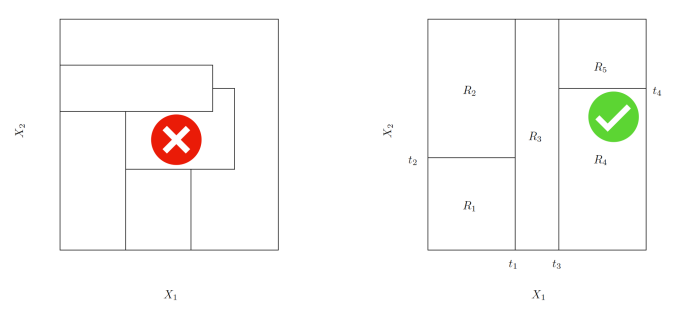
\includegraphics[width=0.72\textwidth]{Images/partition.png}
    \caption{Incorrect vs. Correct Partitioning}
    \label{fig:partition}
\end{figure}

\noindent To grow the tree, CARTs use a greedy fitting algorithm, which means it selects the best split at each step by evaluating all possible features and thresholds. 

\noindent Note: the threshold is the value used to split the data on a feature.

\noindent This decision is made locally and recursively, without considering future splits. The algorithm chooses the split that minimises the RSS:
\[
\sum_{j=1}^J \sum_{i : x_i \in R_j} \left( y_i - \hat{y}_{R_j} \right)^2,
\]
where \( \hat{y}_{R_j} \) is the mean response for the training observations within the \( j \)-th rectangle.

A regression tree is used as the responses in the equity fund dataset are continuous. A regression tree assigns a value to each feature space, $R_j$. This means that the model predicts the output (i.e. which feature space) based on the average response values for all observations in that subgroup.

The greedy fitting algorithm provides good predictions for the training data but may overfit said data, resulting in poor performance on the test dataset. However, pruning can mitigate this issue. Pruning involves removing branches that contribute little to the tree's prediction accuracy to control the bias–variance trade-off. This is either based on a validation set or a complexity penalty.

A common approach to pruning is the weakest link pruning algorithm. This algorithm introduces a non-negative tuning parameter for regression trees, $\alpha$, which minimises the following cost-complexity objective:
\[
\sum_{j=1}^{|T|} \sum_{i : x_i \in R_j} (y_i - \hat{y}_{R_j})^2 + \alpha |T|,
\]
where $|T|$ is the number of terminal nodes (or the size) of the tree $T$.

\subsection{Bagging for Classification and Regression Trees}
Although CARTs are easy to interpret and are similar to standard decision-making processes, the trees generally have high variance. This means that small sample changes lead to significant changes in the fit, and they tend to have poor predictive accuracy. Bootstrap aggregating, also known as bagging, improves the stability and accuracy of CART algorithms by averaging models. Bagging helps reduce variance and avoid over-fitting, but the model becomes more challenging to interpret.

\noindent For regression trees, all the predictions are averaged to obtain:
\[
\hat{f}_{\text{bag}}(x) = \frac{1}{B} \sum_{b=1}^B \hat{f}^b(x),
\]
where \( B \) is the total number of bootstrap samples (i.e. the number of trees trained), and \( \hat{f}^b(x) \) is the prediction from the \( b \)-th tree.

Bagging for CART addresses the overfitting issue in two ways: it can grow large trees with minimal (or no) pruning and rely on the averaging effect of bagging to reduce variance, or alternatively, it can prune each tree individually.

Bagging is advantageous when there is a large amount of data, as is the case here for the equity fund dataset. This is because the empirical distribution will be closer to the actual underlying population's distribution. Additionally, it is the best option when the aim is to minimise the variance of a predictor. 

However, bagging also brings some disadvantages. Firstly, interpretability is lost as the final estimate is not a tree. Secondly, it is an ensemble prediction, i.e. multiple trees are combined to make the final prediction.\cite{DataScienceProcess2019} Also, bagged trees are inherently correlated. This is problematic because the more correlated the random variables are, the smaller the variance reduction of their average, which can undermine one of the key advantages of bagging. 

\subsection{Random Forests}
\label{rf}
Random Forests make bagged CART models more independent, improving variance reduction in their ensemble predictions. They do this by resampling observations and restricting the model to random subspaces, $\mathcal{X}' \subset \mathcal{X}$. This ensures the tree explores different parts of the data, meaning the ensembles are more diverse and hence influential.\cite{breimanstatistics, ho1998random}

The Random Forests algorithm is used in the following way: a bootstrap resample \((y_i^*, x_i^*)_{i=1}^n\) is taken of the training data, like for bagging. Then, the tree is built and each time a split in a tree is considered, \(m\) predictors are randomly selected out of the full set of \(p\) predictors as split candidates, and the best split within those \(m\) predictors is found. Finally, the first two steps are repeated, averaging the prediction of all the regression forest trees.

Random forests are a great option, but they are not interpretable when bagging and using random subspaces. Thus, quantifying the importance of each variable can be difficult. There are two popular approaches which quantify this importance.

One approach is to run a loop over each tree in the forest to determine the significance of each feature variable \(x_j\), where \(j = 1,\dots,p\). Every node that splits on \(x_j\) for each tree is identified, and the improvement in the chosen loss criterion, such as accuracy or the Gini index, is calculated for each split. Each improvement is then summed for every tree in the forest, indicating the significance of \(x_j\).

Another approach is to use out-of-bag (OOB) error estimates, which can be computed via bagging to determine the significance of each feature \(x_j\), where \(j = 1, \dots, p\).\cite{breimanstatistics} For each tree, the OOB samples (i.e. the observations that were not included in the bootstrap sample used to train that tree) are used to evaluate predictive accuracy. To assess the importance of \(x_j\), the entries in the \(j\)-th column of the OOB feature matrix, denoted \(x^{\text{oob}}\), are randomly permuted, breaking the association between \(x_j\) and the rest of the variables. The modified matrix, \(x^{\text{oob}*}\), is then passed through the tree and the resulting change in predictive accuracy is computed. This decrease in accuracy caused by the permutation is averaged across all trees, providing a measure of the importance of feature \(x_j\).

Random forests inherit the advantages of bagging and trees. Thus, tuning is rarely needed. However, they are challenging to implement and have issues with extrapolation.

\noindent Note: tuning for random forests involves adjusting hyperparameters, such as the number of trees or features considered, at each split to optimise predictions.

%\vspace{-0.4cm}
\subsection{Multivariate Regression Trees}
CARTs are limited to single-response regression, making them unsuitable for modelling relationships between multiple correlated responses. Multivariate Regression Trees (MRTs) generalise CARTs by modelling all responses simultaneously and hence accounting for multiple correlated responses.\cite{qcbs_workshop} 

Like CARTs, MRTs also build decision trees by recursively splitting the data into binary partitions along predictor variable thresholds, in order to minimise variability across the response matrix. Ultimately, each split aims to cluster observations that share similar patterns across the responses.\cite{qcbs_workshop} 

MRTs can also be grown until each leaf contains a single observation, but this leads to overfitting. Therefore, trees are pruned using CV, typically selecting the smallest tree within one standard error of the minimum cross-validated error.\cite{death2002multivariate} This is known as the 1-standard error rule.

%By focusing on overall multivariate response similarity, MRTs can uncover how changes in predictors relate to shifts in the joint distribution of response variables. 

However, unlike CARTs, MRTs reveal how relationships between predictors and responses vary across different regions of the predictor space.\cite{qcbs_workshop} Also, unlike univariate regression trees, an MRT returns a vector of predicted responses for each input.

MRTs also adapt the impurity criterion from CARTs to account for all response variables simultaneously, evaluating splits by minimising the total variation across the multivariate response.\cite{death2002multivariate} The impurity measure in MRTs minimises this total variance, and it is the total sum of squares of the responses around the multivariate mean at each node:
\[
\text{impurity} = \sum_{i=1}^{n} \sum_{j=1}^{m} \left( y_{ij} - \bar{y}_j \right)^2,
\]
where $y_{ij}$ represents the $j$-th response for the $i$-th sample, and $\bar{y_j}$ is the mean response at the node.\cite{questier2005cart} 

Because impurity minimisation is performed over the joint space, MRTs naturally cluster correlated responses, and thus, preserving their multivariate response structure. However, MRTs do not explicitly model changes in the covariance structure across predictor values.

MRTs are also highly interpretable, with each node representing a split on a predictor variable, and each leaf corresponding to a distinct cluster. This makes it straightforward to visualise local interactions and the influence of predictors. However, different visualisation tools are needed for MRTs to interpret their results. For instance, at each node of the tree, a histogram shows the distribution of each response within that node, helping to visualise the multivariate outcomes and understand the impact of splits on all responses jointly.\cite{questier2005cart} 

In Figure~\ref{fig:MRT}, the left panel visualises the MRT setup: a response matrix, with two continuous response variables \( Y_1 \) and \( Y_2 \), is regressed on a set of predictors \( X_1, X_2, X_3 \), shown as distinct columns in the predictor matrix. The right-hand panel displays the fitted MRT, where each internal node represents a binary split on one of the predictors. Each terminal node contains a bar plot showing the mean values of \( Y_1 \) and \( Y_2 \) for the observations within that group. This helps assess how each split affects the joint distribution of responses. %Although the response variables are continuous, bar plots are used rather than histograms, in accordance with the original MRT framework \citep{death2002mrt}, to summarise joint response patterns across splits. This visualisation aids interpretation by illustrating how each split differentiates subsets of the data based on changes in the mean structure of the response variables.


\begin{figure}[H]
    \centering
    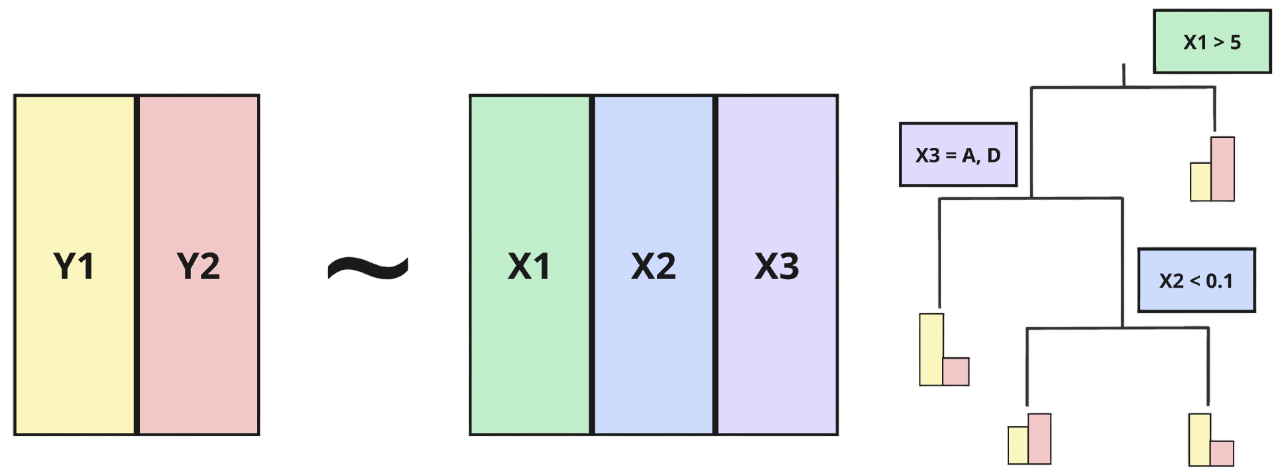
\includegraphics[width=0.8\linewidth]{Images/MRT Image.png}
    \caption{MRT Splitting.\cite{qcbs_workshop}}
    \label{fig:MRT}
\end{figure}

\noindent Note: if a terminal node contains fewer bars than the number of responses, this indicates that one or more response variables have a mean of zero within that group. In other words, bars are only displayed for response variables whose node-wise means are non-zero.


Although MRTs improve on CARTs in MRR, they come with some drawbacks. One such drawback is the inherent instability of tree-structured predictors caused partly by the split function's greedy optimisation.\cite{questier2005cart} Multivariate random forests can be used instead, to resolve this issue.

\subsection{Multivariate Random Forests}
Multivariate Random Forests (MRFs), like univariate random forests, extend MRTs by constructing an ensemble of them through bootstrap and random predictor subsampling.\cite{segal2011multivariate}

The only change from the random forest algorithm in Subsection~\ref{rf} not covered by MRTs is that the bootstrap resample is now taken over \((\mathbf{y}_i^*, x_i^*)_{i=1}^n\) as there are multiple responses to consider.

However, while MRFs are a great extension of MRTs, they exhibit an important limitation in MRR. Although their loss function can be adjusted to implicitly consider response correlations, MRFs do not explicitly force each split to lead to a meaningful change in the response covariance structure. As a result, when responses are highly correlated, MRFs
fail to consider the correlations optimally when building trees, potentially leading to suboptimal splits.\cite{segal2011multivariate} Covariance Regression with Random Forests, however, forces each split to lead to a meaningful change in the response covariance structure.

\subsection{Covariance Regression with Random Forests}
Covariance Regression with Random Forests (CRRFs) extend MRFs by incorporating a splitting criterion, which maximises differences in sample covariance estimates between child nodes. 
\noindent Note: A ``child" refers to the rows selected when a decision tree splits at a node.

Unlike MRFs, which focus solely on predicting the conditional mean, CRRFs explicitly account for response intercorrelation. They extend tree-based methods to estimate the conditional covariance matrix of a multivariate response, given a set of predictors.\cite{alakus2023covariance} While CRRFs are designed to estimate covariance structures, they inherently compute the sample response mean at each terminal node. These mean values can be direct response estimates, allowing CRRFs to generate predictions.

Let \( \Sigma_{\mathbf{y}_i} \) be the true conditional covariance matrix of \( \mathbf{y}_i \) (the responses), based on predictors \( \mathbf{x}_i \), and let \( \Sigma_{\mathbf{X}} \) be the collection of all conditional covariance matrices for \( n \) observations:
\[
\Sigma_{\mathbf{X}} = \{ \Sigma_{\mathbf{y}_i} : i = 1, \dots, n \}.\cite{alakus2023covariance}
\]
Also, let \( \hat{\Sigma}_{\mathbf{y}_i} \) be the estimated conditional covariance matrix of \( \mathbf{y}_i \) based on predictors \( \mathbf{x}_i \), and \( \hat{\Sigma}_{\mathbf{X}} \) be the collection of estimated conditional covariance matrices for \( n \) observations.\cite{alakus2023covariance}

First, a random forest is trained with the set of predictors \( \mathbf{X} \) to find subgroups of observations with similar covariance matrices of \( \mathbf{Y} \), using decision trees to uncover the data structures. These trees are built with a splitting criterion that will be defined later.\cite{alakus2023covariance} The tree-growing process follows the CART algorithm, which aims to obtain subgroups of observations with distinct covariance matrices.\cite{breiman1984classification} Hence, a customised splitting rule at each node is used to increase the difference in covariance matrices between two child nodes in the tree.\cite{moradian2017l_1, tabib2020non, alakucs2021conditional, athey2019generalized}

Before defining this splitting rule, let us first set up some notation. \( \boldsymbol{\hat{\Sigma}}^{L} \) is the sample response covariance matrix estimate,  so $\hat{\Sigma}_{\mathbf{y}_i}$ of the left node, which is written as follows:
\[
\boldsymbol{\hat{\Sigma}}^{L} = \frac{1}{n_L - 1} \sum_{i \in t_L} (\mathbf{y}_i - \bar{\mathbf{Y}}_L)(\mathbf{y}_i - \bar{\mathbf{Y}}_L)^\top,
\]
where \( t_L \) is the set of indices (or the positions within the original data) of the observations in the left node, \( n_L \) is the left node size, and: 
\[
\bar{\mathbf{Y}}_L = \frac{1}{n_L} \sum_{i \in t_L} \mathbf{y}_i.\cite{alakus2023covariance}
\]
The estimate of the sample response covariance matrix for the right node, \( \boldsymbol{\hat{\Sigma}}^{R} \), is calculated similarly, where $t_R$ is the set of indices of observations in the right node and \( n_R \) is its size. 

\noindent The splitting criterion of CRRF is:
\begin{equation}
\sqrt{n_L n_R} \times d(\boldsymbol{\hat{\Sigma}}^{L}, \boldsymbol{\hat{\Sigma}}^{R}),
\label{eq:splitting}
\end{equation}
\noindent where \( d(\boldsymbol{\hat{\Sigma}}^{L}, \boldsymbol{\hat{\Sigma}}^{R}) \) is the Euclidean distance between the upper triangular part of the two matrices, and is computed as follows:
\[
d(\mathbf{D}, \mathbf{E}) = \sqrt{\sum_{i=1}^{q} \sum_{j=i}^{q} (D_{ij} - E_{ij})^2},
\]
where \( \mathbf{D}_{q \times q} \) and \( \mathbf{E}_{q \times q} \) are symmetric matrices. \cite{alakus2023covariance}
The best split among those possible is the one that maximises Equation~\ref{eq:splitting}. This split is what facilitates CRRF as an MRR model, as it explicitly uses a response covariance-based splitting criterion. 

\noindent The final covariance matrices are estimated using random forests. For a new observation, nearest neighbour observations are used to estimate the response mean and final covariance matrix, ensuring both the predicted value and its uncertainty are captured.\cite{alakus2023covariance} This set of observations is called the Bag of Observations for Prediction (BOP). 

For a new observation \( \mathbf{x}^* \), the set of nearest neighbour observations is formed with the oob observations.\cite{lu2021unified, alakus2021rfpredinterval} The \( BOP_{oob} \) for a new observation is:
%\vspace{-0.7cm}
\[
BOP_{oob}(\mathbf{x}^*) = \bigcup_{b=1}^{B} O_b(\mathbf{x}^*),
\]

\noindent where \( B \) is the number of trees and \( O_b(\mathbf{x}^*) \) is the set of oob observations in the same terminal node as \( \mathbf{x}^* \) in the \( b \)th tree, and each tree is built with a selected random sub-sample.\cite{alakus2023covariance}

After training the random forest with the new split for a new observation \( \mathbf{x}^* \), we form \( BOP_{oob}(\mathbf{x}^*) \), which is key for response prediction.\cite{alakus2023covariance} The response mean and covariance matrix are then estimated using the sample mean and covariance matrix of the observations in \( BOP_{oob}(\mathbf{x}^*) \), respectively:
\[
\hat{\mathbf{Y}}^* = \frac{1}{|BOP_{oob}(\mathbf{x}^*)|} \sum_{i \in BOP_{oob}(\mathbf{x}^*)} y_i,
\]
\[
\hat{\mathbf{\Sigma}}_\mathbf{Y}^* = \frac{1}{|BOP_{oob}(\mathbf{x}^*)| - 1} \sum_{i \in BOP_{oob}(\mathbf{x}^*)} (y_i - \hat{\mathbf{Y}}^*)(y_i - \hat{\mathbf{Y}}^*)^\top,
\]
where $y_i$ is an observation from $BOP_{oob}(\mathbf{x}^*)$, \( \hat{\mathbf{Y}}^* \) is the predicted response mean, and \( \hat{\mathbf{\Sigma}}_\mathbf{Y}^* \) represents the estimated conditional covariance matrix of the responses given $\mathbf{x}^*$.

\section{Application}

\subsection{Small-Scale Example}
We will work with this familiar dataset again:
\setlength{\tabcolsep}{4pt} % Adjust column spacing
\begin{table}[H]
    \centering
    \begin{tabular}{|c|c|c|c|}
        \hline
        \( X_1 \): Hours Studied & \( X_2 \): Time Spent on Papers & \( Y_1 \): Math Scores & \( Y_2 \): Science Scores\\
        \hline
        5  & 2  & 78 & 80 \\
        7  & 3  & 85 & 79 \\
        8  & 4  & 88 & 88 \\
        3  & 1  & 65 & 70 \\
        10 & 5  & 92 & 74 \\
        \hline
    \end{tabular}
    \caption{Study Time vs. Exam Scores}
    \label{tab:study_scores5}
\end{table}
%\vspace{-0.8cm}

\noindent Each tree is trained on a bootstrap sample, which is obtained by randomly drawing observations with replacements from the original dataset. 
For the provided dataset, a possible bootstrap sample could be, for example, rows 1,1,2,4 and 5. Here, you can see that row 1 has been repeated, and row 3 has been left out. Another possible bootstrap sample is just getting each row once, so rows 1,2,3,4 and 5. This corresponds to:
\[
\mathbf{X} = 
\begin{bmatrix} 
(5,2,78,80) \\
(7,3,85,79) \\
(8,4,88,88) \\
(3,1,65,70) \\
(10,5,92,74) 
\end{bmatrix}.
\]
After constructing a bootstrap sample, recursive partitioning is performed by selecting the split that maximises the scaled Euclidean distance between the covariance matrices of the left and right child nodes. The Euclidean distance is computed as:
\begin{equation}
d(\mathbf{\Sigma}^L, \mathbf{\Sigma}^R) = \sqrt{\sum_{i=1}^{q} \sum_{j=i}^{q} (\mathbf{\Sigma}^L_{ij} - \mathbf{\Sigma}^R_{ij})^2},    
%\label{eq:Euclid}
\end{equation}
\noindent where \( \mathbf{\Sigma}^L \) and \( \mathbf{\Sigma}^R \) are the empirical covariance matrices of the left and right nodes, respectively. 

In reality, the CRRF will evaluate all possible splits and compute Equation~\ref{eq:splitting} but for simplicity, let us assume the split that maximises this equation is \( X_1 < 7 \). It is important to understand how Equation~\ref{eq:splitting} is computed for any split. First, let us show how this is done for \( X_1 < 7 \). This starts by splitting the data into 2 child nodes: left and right. The left child node contains the observations and responses of:
\[
\mathbf{X}_L = 
\begin{bmatrix} 
5 & 2 & 78 & 80 \\ 
3 & 1 & 65 & 70 
\end{bmatrix},
\]
and the right child node contains:
\[
\mathbf{X}_R = 
\begin{bmatrix} 
7 & 3 & 85 & 79 \\ 
8 & 4 & 88 & 88 \\ 
10 & 5 & 92 & 74 
\end{bmatrix}.
\]
For each node, the mean response is computed as:
\[
\mathbf{\bar{Y}}_L = \frac{1}{2} \sum \mathbf{Y}_L = 
\begin{bmatrix} 
71.5 & 75 
\end{bmatrix}, \quad 
\mathbf{\bar{Y}}_R = \frac{1}{3} \sum \mathbf{Y}_R = 
\begin{bmatrix} 
88.33 & 80.33
\end{bmatrix}.
\]
The covariance matrices are then estimated using:
\[
\mathbf{\Sigma}^L = \frac{1}{n_L - 1} \sum_{i \in L} (\mathbf{Y}_i - \mathbf{\bar{Y}}_L)(\mathbf{Y}_i - \mathbf{\bar{Y}}_L)^\top, \quad 
\mathbf{\Sigma}^R = \frac{1}{n_R - 1} \sum_{i \in R} (\mathbf{Y}_i - \mathbf{\bar{Y}}_R)(\mathbf{Y}_i - \mathbf{\bar{Y}}_R)^\top.
\]
The computed covariance matrices for the left and right nodes are:
\[
\mathbf{\Sigma}^L = 
\begin{bmatrix} 
142.25 & 105.25 \\ 
105.25 & 97.25 
\end{bmatrix}, \quad 
\mathbf{\Sigma}^R = 
\begin{bmatrix} 
41.67 & -10.67 \\ 
-10.67 & 21 
\end{bmatrix}.
\]
Applying the Euclidean distance formula to these matrices gives: 
\[
d(\mathbf{\Sigma}^L, \mathbf{\Sigma}^R) = \sqrt{(142.25-41.67)^2 + 2(105.25 - (-10.67))^2 + (97.25 - 21)^2} = 206.89.
\]
Finally, the scaled Euclidean distance is:
\[
\sqrt{n_L n_R} \times d(\boldsymbol{\hat{\Sigma}}^{L}, \boldsymbol{\hat{\Sigma}}^{R}) = 206.89\sqrt{2 \times 3}=506.77
\]
Since CRRF selects the split that maximises this distance, we can see the split at \( X_1 = 7 \) does lead to a large Euclidean distance between the response sample covariance matrices of each child node.

When predicting, each new observation is assigned to a terminal node based on its feature values. The prediction is computed using the BOP within the same node. For a new test point \( \mathbf{x}^* = (6,3) \), which falls into the left node, the relevant BOP observations here are: 
\[
BOP_{oob}(\mathbf{x}^*) = \{(78,80), (65,70)\}.
\]
The predicted mean response is then given by:
\[
\mathbf{\hat{Y}}^* = \frac{1}{|BOP_{oob}(x^*)|} \sum_{i \in BOP_{oob}(x^*)} \mathbf{Y}_i = 
\begin{bmatrix} 
71.5 \\ 
75 
\end{bmatrix}.
\]
This predicted mean response will then be used to compute the ANRMSE.

\noindent The covariance structure of the predictions can then be estimated as follows:
\[
\mathbf{\hat{\Sigma}}^*_\mathbf{Y} = \frac{1}{|BOP_{oob}(x^*)| - 1} \sum_{i \in BOP_{oob}(x^*)} (\mathbf{Y}_i - \mathbf{\hat{Y}}^*)(\mathbf{Y}_i - \mathbf{\hat{Y}}^*)^\top.
\]
Here, $|BOP_{oob}(x^*)| = 2$. Therefore, $\mathbf{\hat{\Sigma}}^*_\mathbf{Y}$ is:
\[
\mathbf{\hat{\Sigma}}^*_\mathbf{Y} = 
\begin{bmatrix} 
142.25 & 105.25 \\ 
105.25 & 97.25 
\end{bmatrix}.
\]
In this case, the prediction $\mathbf{\hat{Y}^*}$ and its covariance matrix $\mathbf{\hat{\Sigma}}^*_\mathbf{Y}$ correspond to $\mathbf{\bar{Y}}_L$ and $\mathbf{\Sigma}^L$ respectively, because only one tree has been made. For CRRF, many trees are formed from multiple bootstraps because each bootstrap leads to different splits being determined to maximise the Euclidean distance. As a result, the output $\mathbf{\hat{Y}^*}$ will be adjusted when more and more trees are added.

\subsection{Code Explanation}
\label{CRRF Code}
No changes were made to the dataset beyond the exploratory data analysis presented in Chapter~\ref{EDA}, as CRRF is a non-parametric model. Therefore, it does not require preprocessing steps such as frequency encoding (unlike MRLR, RRRR and MRCE).

CRRFs come with a pre-set package in R called \texttt{CovReg}, which enables mean extraction, but there were still some necessary considerations to be made.

To prevent over-fitting, explicit stopping criteria were implemented in the tree growth process. A node was set as terminal if either the depth limit of the tree was reached, \texttt{depth = 0}, or the number of samples in the node fell below the threshold, $n < 5$. In these cases, the node retained the mean and covariance of the responses, rather than splitting further. This procedure stopped the tree from becoming too large and avoided overfitting.

Furthermore, to evaluate the performance of CRRF, a 5-fold CV was implemented using the ANRMSE. The data was randomly split into 5 folds of equal size, where each fold was used as a validation set once, and the remaining 4 folds formed the training set. This ensured that every observation was used in training and validation. At the end of the CV, the final ANRMSE of all the test folds was used to measure CRRF fit.

Parallelisation was also implemented within the CRRF because it uses multi-threading to speed up training by running multiple trees concurrently rather than sequentially. Parallel computing makes programs and processes run faster as more CPUs are used.\cite{azizah2019implementation}

\subsection{Results}
\label{C5 Results}
The CRRF model achieved an ANRMSE of 0.5238, the lowest value thus far. This value was especially surprising given that it did not even consider interaction and polynomial terms. These terms were not explicitly tested as RFs already capture non-linear relationships and interactions through their splits. 

The CRRF model was also analysed in relation to how it determined predictor feature importance in modelling the 2 responses, ROE and sustainability score.

\noindent Note: since MRLR, MRCE, and RRRR return coefficients, they already provide direct insight into predictor-response relationships. In contrast, CRRFs and XGBoost, which will be covered in the next chapter, are non-linear ensemble methods that do not return interpretable coefficients, so feature importance metrics were used to support their interpretation. However, the primary focus of this report remains on evaluating model prediction accuracy.

\begin{figure}[H]
    \centering
    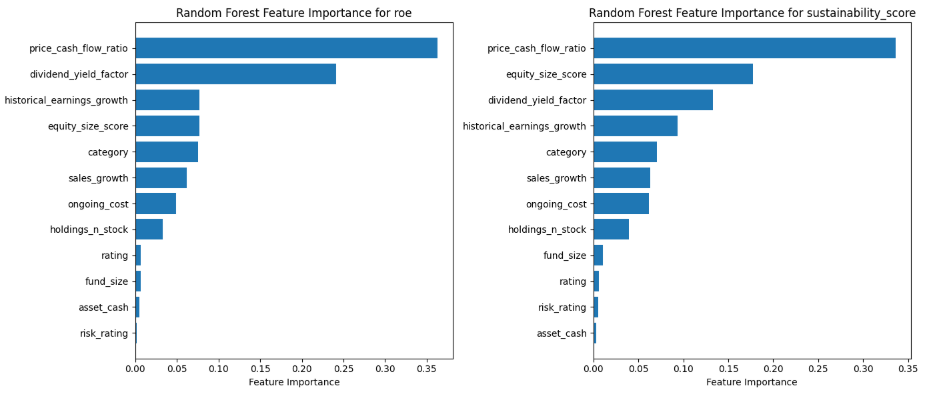
\includegraphics[width=\linewidth]{Plots/rffeatureimportance.png}
    \caption{CRRF Feature Importance}
    \label{fig:crrf_feature_importance}
\end{figure}

\noindent For ROE, the CRRF model gave the highest feature importance to \texttt{price\_cash\_flow\_ratio}, \texttt{dividend\linebreak\_yield\_factor} and \texttt{historical\_earnings\_growth}. Therefore, these features led to the most significant ROE-related covariance changes.  In contrast, \texttt{risk\_rating} and \texttt{asset\_cash} had minimal influence, implying they did not meaningfully alter ROE-related covariances.

For the sustainability score, \texttt{price\_cash\_flow\_ratio} again had the highest feature importance, reinforcing its role in separating subgroups with differing response covariances. \texttt{equity\_size\_score} became more relevant here, which implies that it determined sustainability-related covariance changes more than for ROE. \texttt{historical\_earnings\_growth} and \texttt{dividend\_yield\_factor} remained relevant (from ROE) but with a smaller effect compared to \texttt{price\_cash\_flow\_ratio}. \texttt{sales\_growth} remained as important for sustainability score as it was for ROE, and \texttt{risk\_rating} still had minimal importance.

Overall, the consistent importance of \texttt{price\_cash\_flow\_ratio} highlights its strong role in dictating which equity funds should be invested in long-term, based on the CRRF. 

Meanwhile, features with minimal covariance impact across both responses, like \texttt{risk\_rating} and \texttt{asset\_cash}, should not be prioritised at all. 

Although CRRF has modelled this dataset well, they have some drawbacks. First, they are computationally intensive because they need to calculate covariance matrices at each split. Second, although CV mitigates this somewhat, they are prone to over-fitting with irrelevant features. XGBoost can deal with these issues because it uses approximate tree learning and has built-in regularisation.

\chapter{XG Boost}
\label{xgboost}
This chapter investigates Extreme Gradient Boosting by first explaining its principles in the single-response case, including how it improves upon traditional gradient boosting. % by fitting trees sequentially to residuals. 
This method is then extended to the multivariate case using the Cholesky Decomposition to decorrelate the responses prior to fitting. The resulting model is then evaluated on the equity fund dataset to assess its performance.

\section{Theory}
Now, we move on to Extreme Gradient Boosting, another non-parametric method, which differs from Random Forests as it builds trees sequentially rather than independently. While Random Forests rely on bagging to reduce variance, XGBoost fits each new tree to the negative gradients of the loss function with respect to the current model's predictions. This iterative process forms an ensemble, refining predictions at every step.

\subsection{Introduction}
Gradient tree boosting builds a model by sequentially adding regression trees to minimise a predefined loss function. Each new tree is trained on the negative gradient of the current model, enabling the ensemble to iteratively refine its predictions.\cite{chen2016xgboost}

Formally, for a dataset with \( n \) observations and \( m \) features,
%For a dataset with \( n \) examples and \( m \) features, gradient tree boosting builds a model by combining multiple decision trees
we write:
\[
\mathcal{D} = \{(\mathbf{x}_i, y_i)\}, \quad \mathbf{x}_i \in \mathbb{R}^m, \; y_i \in \mathbb{R}, \quad i = 1, \dots, n.
\]
The prediction for each input, \( \mathbf{x}_i \), is the sum of \( K \) regression trees:
\begin{equation}
\hat{y}_i = \phi(\mathbf{x}_i) = \sum_{k=1}^K f_k(\mathbf{x}_i), \quad f_k \in \mathcal{F},
\label{XGBoost Prediction}
\end{equation}
where each $f_k$ is an individual regression tree in the ensemble, and \( \mathcal{F} \) is the space of all possible regression trees.\cite{chen2016xgboost}

One immediate point of concern is that the estimate will keep increasing as the number of regression trees increases. However, each function \( f_k \) is not an independent prediction of \( y_i \) but rather a correction term trained to minimise the loss function with respect to the ensemble’s current prediction. 

For a general loss function \( \ell(y_i, \hat{y}_i) \), this correction corresponds to the negative gradient, $g_i$, of the loss with respect to the current prediction:
\[
f_k(\mathbf{x}_i) \approx -\frac{\partial \ell(y_i, \hat{y}_i)}{\partial \hat{y}_i}\Big|_{\hat{y}_i = \hat{y}_i^{(t-1)}}=-g_i,
\]
where the superscript \( (t - 1) \) denotes the prediction from the previous iteration of the boosting process, i.e., the ensemble after \( t - 1 \) trees have been added.

\noindent In the case of the squared error loss function:
\begin{equation}
\ell(y_i, \hat{y}_i) = \frac{1}{2}(y_i - \hat{y}_i)^2,
\label{residual}
\end{equation}
the negative gradient simplifies to the residual \( y_i - \hat{y}_i^{(t-1)} \).


The space of all possible regression trees can be formally written as:
\begin{equation}
\mathcal{F} = \left\{ f(\mathbf{x}) = w_{q(\mathbf{x})} \;\middle|\; q : \mathbb{R}^m \rightarrow \{1, \dots, T\}, \; w \in \mathbb{R}^T \right\},
\label{regression tree space}
\end{equation}
where \( T \) is the number of leaves in the tree, \( q \) is a function that maps an input \( \mathbf{x} \) to its corresponding leaf index, and \( w \in \mathbb{R}^T \) is a vector of leaf weights.\cite{chen2016xgboost} Each weight \( w_j \) corresponds to a real-valued score assigned to leaf \( j \). Therefore, the leaf weights are the prediction scores returned by the tree. When an input \( \mathbf{x}_i \) is passed through the tree, \( q \) maps it to a specific leaf \( q(\mathbf{x}_i) \), and the tree returns the corresponding score \( w_{q(\mathbf{x}_i)} \) as its prediction. 

Unlike classification trees, which assign a discrete class label to each leaf, regression trees output continuous values, often referred to as prediction scores, at each leaf. These values are learned during training and represent the model’s prediction for any inputs that fall into their corresponding leaves.

%For any input $\mathbf{x}_i$, the model follows a sequence of decision rules to reach a specific leaf node, which contains a prediction score, where $w_i$ represents the score on the i-th leaf. Therefore, this score becomes the output of the tree for that input.

Building on Equations~\ref{XGBoost Prediction} and \ref{regression tree space}, each regression tree has its own structure, \( q^{(k)} \), and set of leaf scores, \( w^{(k)} \).\cite{chen2016xgboost} Hence, the final model prediction is the sum of these scores across all trees:
\[
\hat{y}_i = \sum_{k=1}^K w^{(k)}_{q^{(k)}(\mathbf{x}_i)}.
\]
%Each new tree improves the model's prediction by fitting to the residuals, thereby reducing the overall error iteratively.\cite{chen2016xgboost}
Extreme Gradient Boosting, otherwise known as XGBoost, improves gradient boosting by including regularisation explicitly in the loss function to address over-fitting and improve model predictions. Its objective function is:
\begin{equation}
    \mathcal{L}(\phi) = \sum_{i=1}^n l(y_i, \hat{y}_i) + \sum_{t=1}^T \Omega(f_t),
    \label{XGBoost Loss}
\end{equation}
where \( l \) represents the loss function, and \( \Omega(f_t) \) is a regularisation term.\cite{chen2016xgboost} The loss function in XGBoost regression can take various forms, such as the log loss. For this report, however, the unscaled squared error loss was used due to its simplicity in gradient derivation (see Equation~\ref{residual}). 

\noindent Note: the omission of the $\frac{1}{2}$ has no impact on model performance, as the constant does not affect the direction of the gradient or the speed of convergence.

XGBoost uses regularisation to help control model complexity and mitigate over-fitting as follows:
\[
\Omega(f_t) = \gamma T + \frac{1}{2} \lambda \sum_{j=1}^T w_j^2,
\]
where \( T \) is the number of leaves in the tree, \( w_j \) are the leaf weights, \( \gamma \) is the pruning parameter which penalises additional leaves, and \( \lambda \) controls the regularisation of leaf weights.\cite{chen2016xgboost}  

The pruning parameter can be selected automatically via CV or hyper-parameter tuning. However, it is ultimately set by the user.
See Equation~\ref{gain} for more on this parameter.

These weights are what XGBoost aims to determine, as they comprise the prediction values assigned to each leaf. XGBoost computes them using the Approximate Greedy Split-Finding Algorithm (see Subsection~\ref{iterative} for more on this).

XGBoost also incorporates shrinkage and column subsampling to reduce overfitting further. Shrinkage scales the leaf weights of newly added trees by a factor of \( \eta \in (0, 1] \), known as the learning rate. This reduces the influence of each individual tree, giving subsequent trees more room to improve the model incrementally.\cite{chen2016xgboost}

\noindent Column subsampling, in which only a random subset of features is considered when constructing each tree, not only acts as a form of regularisation but also improves parallel algorithm computation.\cite{chen2016xgboost}

\noindent Note: this algorithm was implemented in the CRRF (see Subsection~\ref{CRRF Code}).

XGBoost optimises the objective function using a second-order Taylor expansion. With constant terms omitted, the loss function at iteration \( t \) is approximated as:
\[
\mathcal{L}^{(t)} \approx \sum_{i=1}^n \left[ g_i f_t(x_i) + \frac{1}{2} h_i f_t(x_i)^2 \right] + \Omega(f_t),
\]
where \( g_i = \partial_{\hat{y}_{i}^{(t-1)}} l(y_i, \hat{y}_{i}^{(t-1)}) \) and \( h_i = \partial_{\hat{y}_{i}^{(t-1)}}^2 l(y_i, \hat{y}_{i}^{(t-1)}) \) are the first and second-order gradients of the loss function, respectively.\cite{chen2016xgboost} 

To construct decision trees, XGBoost evaluates potential binary splits using the Greedy Algorithm for Split Finding. This algorithm involves maximising a gain function:
\begin{equation}
\text{Gain} = \frac{1}{2} \left[ \frac{G_L^2}{H_L + \lambda} + \frac{G_R^2}{H_R + \lambda} - \frac{(G_L + G_R)^2}{H_L + H_R + \lambda} \right] - \gamma.\cite{chen2016xgboost}
\label{gain}
\end{equation}
Each candidate split divides the training data into two subsets based on a feature threshold. The instances satisfying the condition (e.g. \( x_j \leq s \)) are assigned to the left node, while those that do not are assigned to the right node.

Here, \( G_L \) and \( H_L \) are the sums of first and second-order gradients for the left child ($L$) node, \( G_R \) and \( H_R \) are the corresponding sums for the right child ($R$) node, \( \lambda \) is a regularisation parameter, and \( \gamma \) is the pruning parameter.\cite{chen2016xgboost} 

\noindent Note: A ``child" refers to the rows selected when a decision tree splits at a node. 

Equation~\ref{gain} means that a node will only be split if the gain in the objective function exceeds the pruning parameter, \( \gamma \). Higher values of \( \gamma \) encourage shallower trees by penalising complexity.

In simplified form, the Gain can be written as:
\[
\text{Gain} = \frac{1}{2} \left[ S_L + S_R - S_P \right] - \gamma,
\]
where:
\[
S_L = \frac{G_L^2}{H_L + \lambda}, \quad S_R = \frac{G_R^2}{H_R + \lambda}, \quad S_P = \frac{(G_L + G_R)^2}{H_L + H_R + \lambda}.
\]
Note: Each component within the Gain's bracket is called the (similarity) score and $S_P$ is the score for the parent node of the new node being derived.


\subsection{Iterative Steps of XGBoost}
\label{iterative}
As outlined in Chen and Guestrin (2016), the exact Greedy Algorithm occurs by iterating over each feature dimension \( k \), ranging from 1 to \( m \), where \( m \) is the total number of predictors. 

For each feature, potential split points are evaluated by sorting the training instances based on their corresponding feature values. During this process, the cumulative sums of gradients and Hessians for the left child node, denoted \( G_L \) and \( H_L \), are initialised to zero and updated at each step as:
\[ 
G_L \gets G_L + g_j, \quad H_L \gets H_L + h_j.
\] 
The corresponding values for the right child are computed as \( G_R = G-G_L \) and \( H_R = H-H_L \), where \( G \) and \( H \) are the total sums over the parent node.

The quality of each split is evaluated using the gain, which measures the reduction in loss. At each step, the algorithm compares the gain of the current split to the best one found so far:
\[
\text{Gain}_{\text{new}} = S_L + S_R - S_P,
\]
and retains the maximum.

\noindent Note: the pruning parameter \( \gamma \) is only applied after split selection, not during the gain evaluation.

After evaluating all candidate splits, the algorithm selects the one with the highest gain. If no split yields a positive gain, the node remains a leaf.
This approach ensures that each decision tree grows in a way that minimises residual error at each step, leading to more accurate predictions.\cite{chen2016xgboost}

The exact Greedy Algorithm is ideal for XGBoost, but due to its computational cost, an approximate greedy algorithm is used in practice. This method is similar to the prior one, but with some adjustments which are explained below, again from Chen and Guestrin (2016).

The approximate greedy algorithm begins by iterating over each feature dimension \( k = 1, \dots, m \), where \( m \) is the total number of features. 

For each feature \( k \), a set of candidate splits \( S_k = \{ s_{k1}, s_{k2}, \dots, s_{kl} \} \) is proposed by dividing the feature values into percentiles. This ensures the split proposals are distributed evenly across the feature range, capturing key points that are likely to lead to huge loss reduction. Split proposals can be generated globally or locally: in the global setting, split points are selected once per tree and reused at each node, while in the local setting, new split points are computed independently for each node.

After generating the candidate splits, the algorithm evaluates their quality. For each proposed split \( s_{k,v} \) in feature \( k \), the gradients and Hessians of instances falling between two consecutive split points are accumulated. The gradients and Hessians are then computed as:
\begin{align*}
G_{kv} &\gets =\textstyle \sum_{j \in \{ j \mid s_{k,v} \ge \mathbf{x}_{jk} > s_{k,v-1} \}} g_j \\
H_{kv} &\gets =\textstyle \sum_{j \in \{ j \mid s_{k,v} \ge \mathbf{x}_{jk} > s_{k,v-1} \}} h_j
\end{align*}
\noindent where \( G_{kv} \) denotes the sum of gradients, and \( H_{kv} \) the sum of Hessians over the interval between \( s_{k,v-1} \) and \( s_{k,v} \). This process approximates the exact split-finding procedure by evaluating only a limited subset of potential split points.

Once the gradients and Hessians have been computed for all proposed splits, the algorithm selects the split that maximises the gain. This follows the same logic as the exact greedy method but limits evaluation to the proposed split points, significantly reducing computational cost.\cite{chen2016xgboost}

The same procedure described earlier is then applied, but restricted to the proposed splits. While this approximation sacrifices some precision, it greatly improves efficiency, allowing XGBoost to scale to large datasets.

After identifying the optimal split, the corresponding leaf weight is computed as:
\[
w_j = -\frac{G_j}{H_j + \lambda},
\]
where \( G_j \) is the sum of gradients for all instances in the leaf, \( H_j \) is the sum of Hessians for all instances in the leaf, and \( \lambda \) is the regularisation parameter.\cite{chen2016xgboost}

\noindent Each instance’s prediction is updated as follows:
\[
\hat{y}^{(t)} = \hat{y}^{(t-1)} + \eta w_j,
\]
\noindent where \( \hat{y}^{(t-1)} \) represents the previous prediction, \( w_j \) is the weight of the leaf the instance falls into, and \( \eta \) is the learning rate - which controls the step size of updates.\cite{chen2016xgboost}

\subsection{Cholesky Decomposition}
Although a prior distribution is not required to apply Cholesky decomposition, assuming a multivariate normal distribution (MVN), which can be done on the equity fund dataset, helps satisfy its requirements, which are a positive definite symmetric matrix.
The probability density function of an MVN distribution is given by:
 \[
f(\mathbf{Y} | \boldsymbol{\mu_\mathbf{Y}}, \Sigma_{\mathbf{Y}}) = \frac{1}{\sqrt{(2\pi)^D |\Sigma_{\mathbf{Y}}|}} 
\exp \left( -\frac{1}{2} (\mathbf{Y} - \boldsymbol{\mu}_{\mathbf{Y}})^\top 
\Sigma_{\mathbf{Y}}^{-1} (\mathbf{Y} - \boldsymbol{\mu}_{\mathbf{Y}}) \right),
\]
where \( \boldsymbol{\mu}_{\mathbf{Y}} \in \mathbb{R}^D \) represents a vector of conditional means, 
\( \Sigma_{\mathbf{Y}} \) is the positive definite symmetric \( D \times D \) response covariance matrix, $D$ is the number of responses, and \( | \cdot | \) denotes the determinant.\cite{marz2022multi} 

In the bivariate case \( (D = 2) \), the local response covariance matrix for instance \( i \), denoted \( \boldsymbol{\Sigma}_{i\mathbf{y}} \), is:
\[
\mathbf{\Sigma}_{i\mathbf{y}} =
\begin{bmatrix}
\sigma^2_{i,1}(\mathbf{x}) & \rho_i(\mathbf{x}) \sigma_{i,1}(\mathbf{x}) \sigma_{i,2}(\mathbf{x}) \\
\rho_i(\mathbf{x}) \sigma_{i,1}(\mathbf{x}) \sigma_{i,2}(\mathbf{x}) & \sigma^2_{i,2}(\mathbf{x})
\end{bmatrix},
\]
where, for each \( i = 1, \dots, N \), $\rho_i(\mathbf{x})$ is the conditional correlation between the two responses, the diagonal entries represent the variances, and the off-diagonal entries represent the covariances.\cite{marz2022multi}

To ensure positive definiteness of the response covariance matrix, \( \boldsymbol{\Sigma}_{\mathbf{Y}} \), a common and efficient approach is to use the Cholesky decomposition, which factorises the matrix as follows:
\[
\boldsymbol{\Sigma}_{\mathbf{Y}} = \mathbf{L} \mathbf{L}^\top,
\]
where \( \mathbf{L} \in \mathbb{R}^{D \times D} \) is a lower triangular matrix.\cite{marz2022multi} This decomposition guarantees positive definiteness as long as all diagonal elements, \( \ell_{ii} \), of \( \mathbf{L} \) are strictly positive. The \( D(D-1)/2 \) off-diagonal elements, \( \ell_{ij} \) (for \( j < i \)), may take any value in \( \mathbb{R} \). 

The Cholesky decomposition uses the following algorithm to derive $\mathbf{L}$:

\begin{enumerate}
    \item Initialise \( \mathbf{L} \) as an \( n \times n \) zero matrix.
    
    \item For each row \( i \) (from 1 to \( n \)):  
    \begin{itemize}
        \item Compute the diagonal element \( L_{ii} \):
        \[
        L_{ii} = \sqrt{A_{ii} - \sum_{k=1}^{i-1} L_{ik}^2}
        \]
        \item For each column \( j \) (below diagonal, \( j > i \)):
        \[
        L_{ji} = \frac{A_{ji} - \sum_{k=1}^{i-1} L_{jk} L_{ik}}{L_{ii}}
        \]
    \end{itemize}
    
    \item Return \( \mathbf{L} \).
\end{enumerate}
Cholesky decomposition can be used to remove intercorrelation between response variables by applying the transformation \( \mathbf{L}^{-1} \mathbf{Y}^\top \), which produces decorrelated responses.\cite{pollockcholesky} This decorrelation allows XGBoost to be applied independently to each transformed response. After prediction, the original correlated response space is recovered by reapplying \( \mathbf{L} \), which reintroduces the covariance structure.

\vspace{0.1cm}
\noindent Note: There does exist an experimental version of XGBoost, Multi-Output XGBoost, which natively supports MRR. However, its methodology still needs to be fleshed out. For more details on this implementation, see the official XGBoost multi-output regression demo \href{https://xgboost.readthedocs.io/en/stable/python/examples/multioutput_regression.html}{here}.


\section{Application}

\subsection{Small-Scale Example}
We will work with the familiar dataset, evaluating Mathematics and Science Scores:

%\setlength{\tabcolsep}{4pt} % Adjust column spacing
\setlength{\tabcolsep}{4pt} % Adjust column spacing
\begin{table}[H]
    \centering
    \begin{tabular}{|c|c|c|c|}
        \hline
        \( X_1 \): Hours Studied & \( X_2 \): Time Spent on Papers & \( Y_1 \): Math Scores & \( Y_2 \): Science Scores\\
        \hline
        5  & 2  & 78 & 80 \\
        7  & 3  & 85 & 79 \\
        8  & 4  & 88 & 88 \\
        3  & 1  & 65 & 70 \\
        10 & 5  & 92 & 74 \\
        \hline
    \end{tabular}
    \caption{Study Time vs. Exam Scores}
    \label{tab:study_scores6}
\end{table}
\noindent We have:
\[
\mathbf{X} =
\begin{bmatrix}
5 & 7 & 8 & 3 & 10 \\
2 & 3 & 4 & 1 & 5
\end{bmatrix}^{\top},
\quad
\mathbf{Y} =
\begin{bmatrix}
78 & 85 & 88 & 65 & 92 \\
80 & 79 & 88 & 70 & 74
\end{bmatrix}^{\top},
\quad
\mathbf{\bar{Y}} = \begin{bmatrix}
  81.6  & 78.2
\end{bmatrix}^\top.
\]
First,calculate the sample response covariance matrix, $\mathbf{\hat{\Sigma}_Y}$:
\[
\mathbf{\hat{\Sigma}_Y} = \frac{1}{n-1} (\mathbf{Y} - \bar{\mathbf{Y}})^{\top} (\mathbf{Y} - \bar{\mathbf{Y}})=
\begin{bmatrix}
    112.30 & 37.85 \\
    37.85 & 46.20
\end{bmatrix},
\]
This matrix is symmetric and positive definite because its (1,2) and (2,1) entries are the same, and it has positive eigenvalues. Therefore, Cholesky decomposition can be applied.

Next comes the Cholesky Decomposition of the response covariance matrix. This subsection is for clarity, so for ease of computation, let us show Cholesky Decomposition on a ``nicer" matrix:
\[
\mathbf{A} =
\begin{bmatrix}
4 & 2 \\
2 & 3
\end{bmatrix}.
\]
We aim to find a lower triangular matrix \( \mathbf{L} \) such that:
\[
\mathbf{A} = \mathbf{L} \mathbf{L}^\top, \quad
\mathbf{L} =
\begin{bmatrix}
L_{11} & 0 \\
L_{21} & L_{22}
\end{bmatrix}.
\]
The first step is to compute \( L_{11} \) using the formula for diagonal elements:
\[
L_{ii} = \sqrt{A_{ii} - \sum_{k=1}^{i-1} L_{ik}^2}
\Rightarrow
L_{11} = \sqrt{A_{11}} = \sqrt{4} = 2
\Rightarrow
\mathbf{L} =
\begin{bmatrix}
2 & 0 \\
L_{21} & L_{22}
\end{bmatrix}.
\]
Next, compute \( L_{21} \). For off-diagonal elements:
\[
L_{ji} = \frac{A_{ji} - \sum_{k=1}^{i-1} L_{jk} L_{ik}}{L_{ii}} \Rightarrow
L_{21} = \frac{A_{21}}{L_{11}} = \frac{2}{2} = 1
\Rightarrow
\mathbf{L} =
\begin{bmatrix}
2 & 0 \\
1 & L_{22}
\end{bmatrix}.
\]
Finally, compute \( L_{22} \), going back to our diagonal element formula:
\[
L_{ii} = \sqrt{A_{ii} - \sum_{k=1}^{i-1} L_{ik}^2}
\Rightarrow
L_{22} = \sqrt{A_{22} - L_{21}^2} = \sqrt{3 - 1} = \sqrt{2}
\Rightarrow
\mathbf{L} =
\begin{bmatrix}
2 & 0 \\
1 & \sqrt{2}
\end{bmatrix}.
\]
See Subsection~\ref{CD} for verification that this decomposition is correct.

\noindent Applying this algorithm to $\mathbf{\Sigma_Y}$ gives:
\[
\mathbf{\Sigma_Y} = \mathbf{L}\mathbf{L}^\top=
   \begin{bmatrix}
    10.60 & 0 \\
    3.57 & 5.78
   \end{bmatrix}
   \begin{bmatrix}
       10.60 & 3.57 \\
       0 & 5.78
   \end{bmatrix}.
\]
Now, we can decorrelate the responses using $\mathbf{L}^{-1}$:
\[
\tilde{\mathbf{Y}}=
\mathbf{L}^{-1}\mathbf{Y}^\top =
\begin{bmatrix}
7.36 & 8.02 & 8.30 & 6.13 & 8.68 \\
9.29 & 8.71 & 10.09 & 8.32 & 7.43
\end{bmatrix}^\top.
\]
Here, the off-diagonal elements of the covariance matrix of the transformed responses are zero, and it leaves the identity matrix, $\mathbf{I}_2$:
\[
\text{Cov}(\tilde{\mathbf{Y}}) \approx
\begin{bmatrix}
1 & 0 \\
0 & 1
\end{bmatrix}.
\]
Now that the responses are decorrelated, we can apply an independent XGBoost model to each response.

Let us apply XGBoost, with a squared error loss function, to response $\tilde{Y}_1$ (the first column of the decorrelated responses), Mathematics Scores against the predictors $X_1$ and $X_2$.
XGBoost starts by initialising predictions for all samples. The initial prediction is typically 0.5, but let us start here instead by taking the mean of \( \tilde{Y}_1 \):
\begin{equation}
    \frac{7.36 + 8.02 + 8.30 + 6.13 + 8.68}{5}
= \frac{38.49}{5} = 7.70.
\label{initial_prediction}
\end{equation}

\noindent Thus, the initial prediction for all samples is:
\[
\hat{Y}_1^{(0)} =
\begin{bmatrix}
7.70 & 7.70 & 7.70 & 7.70 & 7.70
\end{bmatrix}^\top.
\]
Next, the residuals are calculated as the difference between the actual values (\( \tilde{Y}_1 \)) and the initial predictions (\( \hat{Y}_1^{(0)} \)):
\begin{equation*}
    \begin{aligned}
        r_1 = \tilde{Y}_1 - \hat{Y}_1^{(0)} &=
\begin{bmatrix}
7.36 & 8.02 & 8.30 & 6.13 & 8.68
\end{bmatrix}^{\top}
-
\begin{bmatrix}
7.70 & 7.70 & 7.70 & 7.70 & 7.70
\end{bmatrix}^{\top} \\
&=
\begin{bmatrix}
-0.34 & 0.32 & 0.60 & -1.57 & 0.98
\end{bmatrix}^{\top}.
    \end{aligned}
\end{equation*}
\noindent The residuals are the errors in the initial predictions, which will be used to fit the first XGBoost tree. The residuals are taken because they are half the gradients when using the squared error loss function. The Gradients, $g_i$, and Hessians, $h_i$, are needed because they are critical in evaluating the Score and computing the Gain. The gradients are calculated as:
\[
g_i = \frac{\partial L}{\partial \hat{Y}_i} = \frac{\partial }{\partial \hat{Y}_i}\sum_{i=1}^{n} (\hat{Y}_i - Y_i)^2 = 2(Y_i - \hat{Y}_i)=2r_i,
\]
where the summation vanishes because we are looking at each $i^{\text{th}}$ element when differentiating.

From the residuals, the gradients are:
\[
g =
\begin{bmatrix}
-0.68 &
0.64 &
1.21 &
-3.13 &
1.96
\end{bmatrix}^\top.
\]
For the squared error loss, the second-order gradient (or Hessian) is:
\[
h_i = \frac{\partial^2 L}{\partial \hat{Y}_i^2} = 2.
\]
Since we are using the squared error loss function, the Hessian for all observations is:
\[
h =
\begin{bmatrix}
2 &
2 &
2 &
2 &
2
\end{bmatrix}^\top
\]
Now, we train a small decision tree to predict the gradients. This starts with the parent node, $P$, which contains all the data. Each tree starts with a single leaf, and all residuals go to that leaf.\cite{statquest2019} All that needs to be done here is to compute the score of the leaf using the exact residuals:
\[
S_P = \frac{(\sum g_P)^2}{\sum h_P + \lambda}=0.
\]
where $g_P, h_P$ are the Gradients and Hessians of the parent node, respectively. 

It might be surprising that $S_P=0$. However, this makes sense because, as a result of this loss function, the gradients are proportional to the residuals, which always sum to zero. 

\noindent Note: When the gradients within a node have opposite signs, they tend to cancel each other out, reducing the numerator's contribution in the leaf score formula. This results in a relatively small score. In contrast, when the gradients are similar in direction and magnitude, the summed gradient is large, producing a higher score.\cite{statquest2019}

XGBoost will then evaluate splits after computing the corresponding scores by comparing the Gain for each split in $X_1$ and $X_2$ in this dataset, and finding the split which maximises said Gain. Maximising the Gain means there is a better separation of gradients into clusters with similar values.\cite{statquest2019} 

Iterating through all possible split points is computationally expensive. To address this, XGBoost uses a weighted quantile sketch to approximate the best split points (see Subsection~\ref{WQS} for details). This significantly speeds up training by reducing the number of candidate splits.

Now, let us show how the gain is computed for an example split: $X_1 < 7$, which splits the data into 2 sets of predictors and corresponding transformed responses:
\setlength{\tabcolsep}{4pt} % Adjust column spacing
\begin{table}[H]
    \centering
    \begin{tabular}{|c|c|c|c|}
        \hline
        \( X_1 \): Hours Studied & \( X_2 \): Time Spent on Papers & \( \tilde{Y}_1 \): Mathematics Scores & \( r_1 \): Residuals \\
        \hline
        5  & 2  & 7.36  & -0.34 \\
        3  & 1  & 6.13  & -1.57 \\
        \hline
    \end{tabular}
    \caption{Study Time vs. Mathematics Scores for $X_1 < 7$}
    \label{tab:adjusted_study_scores6a}
\end{table}
\vspace{-0.2cm}
\setlength{\tabcolsep}{4pt} % Adjust column spacing
\begin{table}[H]
    \centering
    \begin{tabular}{|c|c|c|c|}
        \hline
        \( X_1 \): Hours Studied & \( X_2 \): Time Spent on Papers & \( \tilde{Y}_1 \): Mathematics Scores & \( r_1 \): Residuals \\
        \hline
        7  & 3  & 8.02  & 0.32 \\
        8  & 4  & 8.30   & 0.60 \\
        10 & 5  & 8.68  & 0.98 \\
        \hline
    \end{tabular}
    \caption{Study Time vs. Mathematics Scores for $X_1 \geq 7$}
    \label{tab:adjusted_study_scores6b}
\end{table}
\noindent Science Scores, $\hat{Y}_2$, have been removed as we are just modelling $\tilde{Y}_1$ here, and the initial residuals are placed for clarity when calculating the gradients and Hessians. 

\noindent Let us call Table~\ref{tab:adjusted_study_scores6a} the ``left" ($L$) node and Table~\ref{tab:adjusted_study_scores6b} the ``right" ($R$) node. From each node, the cumulative gradients and Hessians are calculated as:
\[
G_L = \sum_{i=1}^{2} 2(r_i)_L=-3.81, \quad H_L = \sum_{i=1}^{2} 2=4, \quad
G_R = \sum_{i=1}^{2} 2(r_i)_R=3.81, \quad H_R = \sum_{i=1}^{3} 2=6.
\]
This is used to calculate the similarity scores for the left and right nodes with $\lambda = 0.1$:
\[
S_L = \frac{G_L^2}{H_L + \lambda}=3.54, \quad S_R = \frac{G_R^2}{H_R + \lambda}=2.38.
\]
Now, compute the Gain for $X_1 < 7$ in comparison with the parent node:
\[
\text{Gain} =  S_L+S_R - S_P = 5.93.
\]
For simplicity, assume the tree split of \( X_1 < 7 \) gives the optimal gain, so we can use it to adjust the predictions. The leaf weight differs by the child node that each row falls in, and is calculated as:
\[
w_L = -\frac{G_L}{H_L + \lambda}=0.93, \quad w_R = -\frac{G_R}{H_R + \lambda}=-0.62
\]
The predictions are then adjusted using the leaf weight with learning rate $\eta$, which we set as 0.3. Here, the initial prediction was the mean, from Equation~\ref{initial_prediction}. So, the final transformed predictions are: 
\[
\hat{Y}_{1,L}^{(1)} = \hat{Y}_1^{(0)}+\eta\times w_L=7.98,\quad \hat{Y}_{1,R}^{(1)} = \hat{Y}_1^{(0)}+\eta\times w_R=7.51.
\]
These need to be converted back to the original response space with the original correlation structure, using: $\mathbf{L}\hat{Y}_{1, L}^{(1)}$ and $\mathbf{L}\hat{Y}_{1, R}^{(1)}$. This gives the following original predictions:
\[
\text{Left Node}: \hat{Y}_{1}^{(1)}=84.55, \quad \text{Right Node}: \hat{Y}_{1}^{(1)}=79.61.
\]
Therefore, when new observations of the form $(X^*_1, X^*_2)$ pass through this first tree, the tree returns $Y^*_1=84.55$ if $X^*_1<7$ and $Y^*_1=79.61$ if $X^*_1 \geq 7$. As more and more splits are evaluated and nodes added to the tree, different observations will produce different responses.

\vspace{-0.3cm}
\subsection{Code Explanation}
No changes were made to the dataset beyond the exploratory data analysis presented in Chapter~\ref{EDA}, as XGBoost, like CRRF, is a non-parametric model. Therefore, it does not require preprocessing steps such as frequency encoding.

The primary implementation detail (which has not been covered thus far) involved using \( k \)-fold CV.
The dataset was partitioned into five folds using \texttt{KFold}, with shuffling enabled to ensure randomness in CV.
For each fold, the empirical response covariance matrix of the target variables was computed using \texttt{numpy.cov} to capture interdependencies between responses. 

Cholesky decomposition was then applied via \texttt{numpy.linalg.cholesky}, producing a lower triangular matrix \( \mathbf{L} \). Its inverse, \( \mathbf{L}^{-1} \), was computed using \texttt{numpy.linalg.inv} to decorrelate the response variables prior to model training.
Each decorrelated response variable was then modelled independently using an XGBoost regression model that was implemented with \texttt{XGBRegressor}.
The models were trained on the transformed responses using \texttt{model.fit(X\_train, Y\_train)}, and predictions were generated on the validation set using \texttt{model.predict(X\_val)}.
As the predictions were produced in the transformed space, they were mapped back to the original scale by multiplying by the Cholesky factor via \texttt{numpy.dot}. This step ensured that the predicted responses retained their original correlation structure. Finally, the adjusted predictions were used to compute the ANRMSE across all folds.



\subsection{Results}
XGBoost achieved an ANRMSE of 0.4267, indicating an excellent fit. This was the best performance among all the models tested and highlights XGBoost’s effectiveness in modelling complex datasets.
\begin{figure}[H]
    \centering
    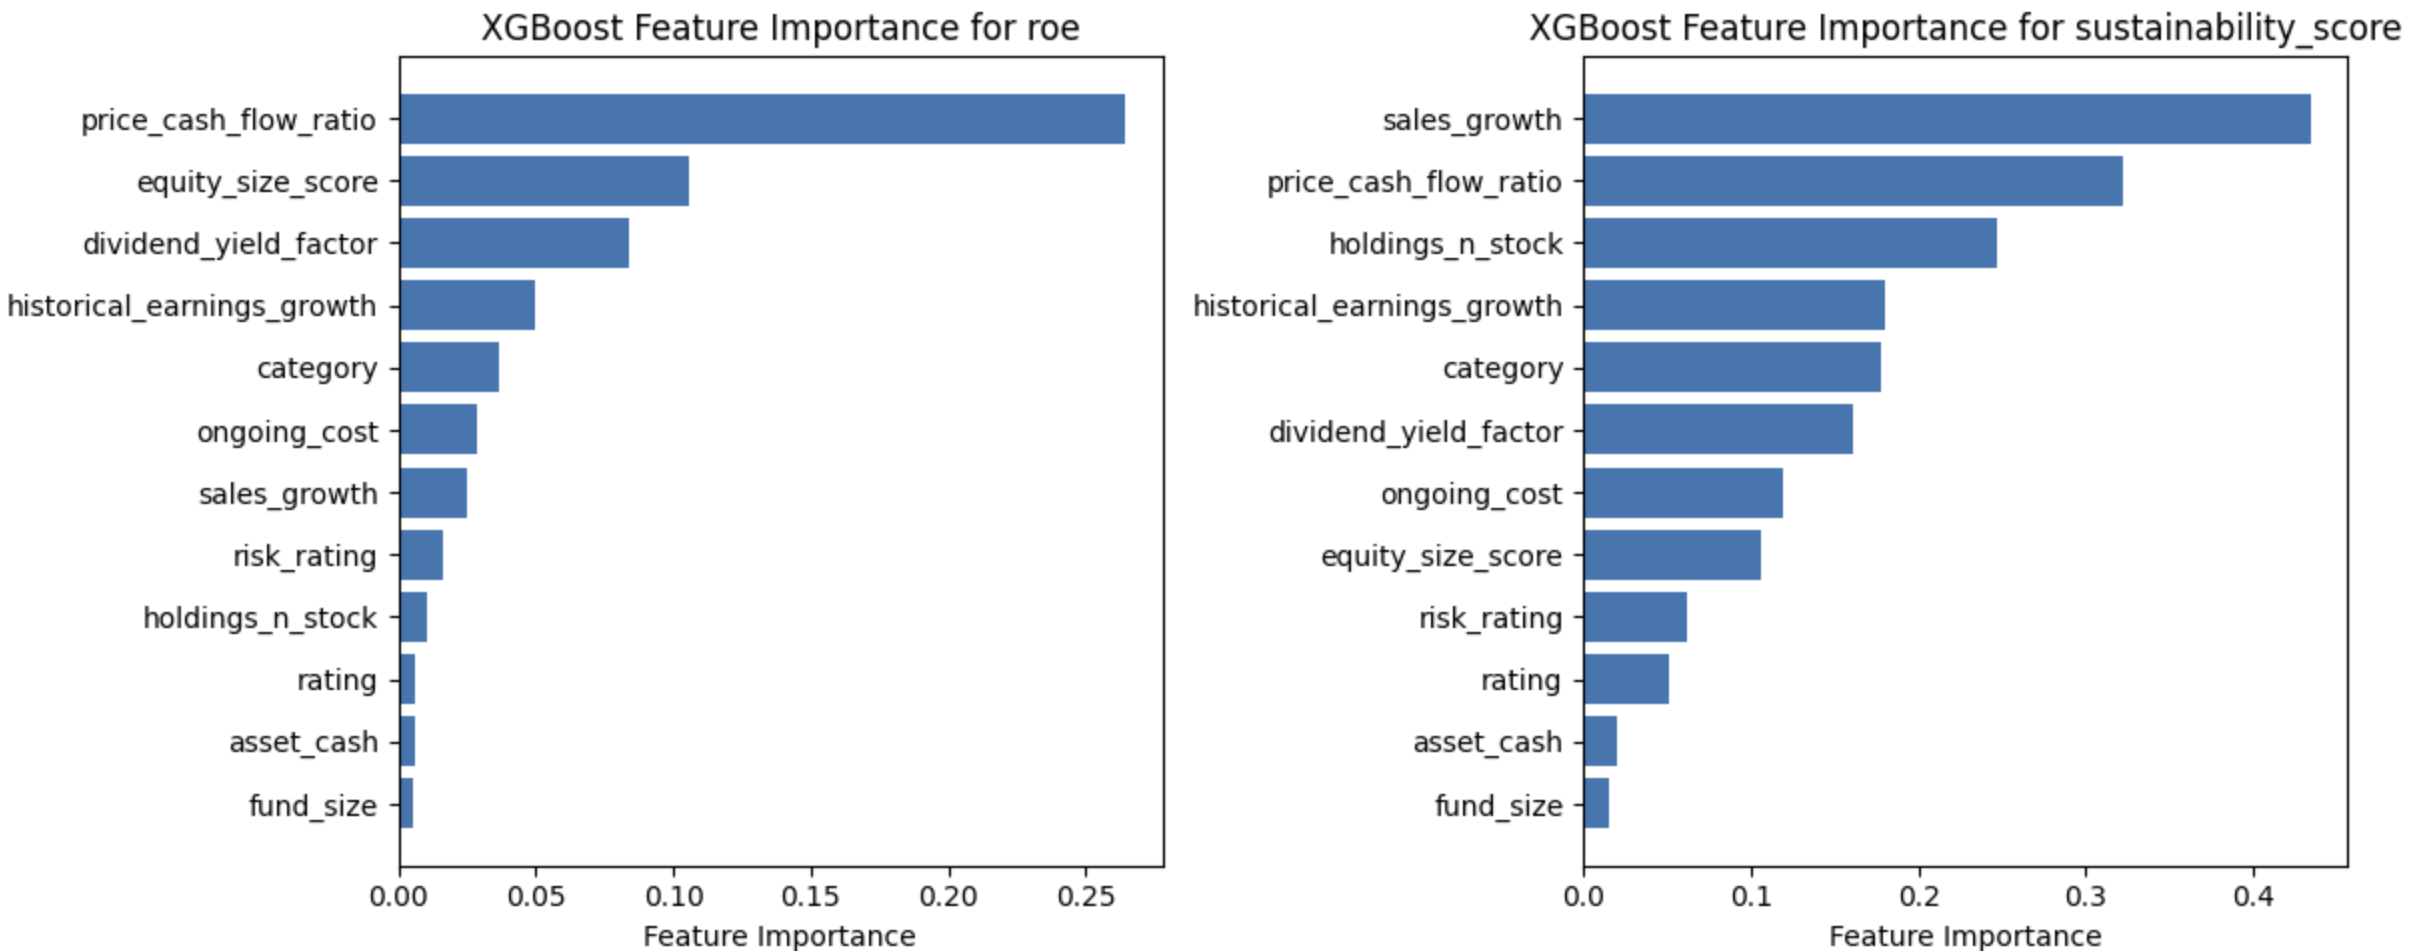
\includegraphics[width=0.9\textwidth]{Plots/XGBoost Feature Importance.png}
    \caption{XGBoost Feature Importance}
    \label{fig:xgboostFI}
\end{figure}
\noindent The most important feature in explaining the ROE was the \texttt{price\_cash\_flow\_ratio}. This means that, following decorrelation, this ratio had the greatest impact in terms of accounting for variation in the response. However, due to the Cholesky transformation, some of its influence may have been partially transferred to the sustainability score when mapping back to the original response space.

Other notable contributors included the \texttt{equity\_size\_score} and the \texttt{dividend\_yield\_factor}, reflecting their substantial role in predicting the decorrelated response. On the other hand, variables such as \texttt{asset\_cash} and \texttt{fund\_size} had relatively low feature importance, indicating that these features provided little additional information once response dependencies had been taken into account.

The most impactful feature for the sustainability score was \texttt{sales\_growth}. Unlike ROE, where a dominant predictor emerged, sustainability appeared to be influenced by a few predictors (such as  \texttt{holdings\_n\_stock} and \texttt{historical\_earnings\_growth}), as indicated by its more even distribution of importance across features. 
The \texttt{price\_cash\_flow\_ratio} again ranked highly, similar to its importance in predicting ROE. This supports the fact that prior to decorrelation, the responses shared some correlation, which was separated using Cholesky decomposition. 

Overall, the consistent importance of \texttt{price\_cash\_flow\_ratio} highlights its strong role in dictating which equity funds should be invested in long-term, based on Cholesky-Decomposed XGBoost (this further supports the suggestion from CRRF - see Subsection~\ref{C5 Results}). Meanwhile, features with minimal impact, like \texttt{fund\_size} and \texttt{asset\_cash}, should not be prioritised. 

Ultimately, XGBoost proved highly effective on the equity fund dataset, but it does bring some limitations. One notable drawback is that, even though feature importance plots can be generated to ease this, interpreting XGBoost can still be challenging due to its inherent complexity.\cite{xgboosting2024}


\chapter{Conclusion}
\section{Summary of Findings and Model Comparisons}
\subsection{Summary of Findings}
Table~\ref{tab:model_fit} provides the key figures generated in this report from the  MRR models:
\begin{table}[h!]
    \centering
    \caption{Model Fit Comparison on Equity Fund Dataset}
    \label{tab:model_fit}
    \renewcommand{\arraystretch}{1.6} % Increase row height
    \setlength{\tabcolsep}{11pt} % Increase column separation
    \begin{tabular}{|l|l|l|} % Add vertical borders for 3 columns
        \hline
        \textbf{\Large Model} & \textbf{\Large ANRMSE} & \textbf{\Large Model Fit} \\
        \hline
        \multicolumn{3}{|c|}{\textbf{Chapter 3: Linear Regression}} \\
        \hline
        Model 1: MRLR with all predictors & 0.7606 & \classifyFit{0.7606} \\
        Model 2: Forward Selection & 0.7606 & \classifyFit{0.7606} \\
        Model 3: Backward Selection & 0.7924 & \classifyFit{0.7924} \\
        Model 4: Bidirectional Selection & 0.7606 & \classifyFit{0.7606}\\
        Model 5: Bidirectional Selection with Interaction Terms & 0.5613 & \classifyFit{0.5613}\\
        Model 6: Bidirectional Selection with Non-Linear Terms & 0.6893 & \classifyFit{0.6893}\\
        \hline
        \multicolumn{3}{|c|}{\textbf{Chapter 4: Shrinkage Methods}} \\
        \hline
        Model 7: MRCE & 0.7612 & \classifyFit{0.7612}\\
        Model 8: RRRR & 0.7510 & \classifyFit{0.7510}\\
        Model 9: MRCE including Polynomial Terms & 0.6781 & \classifyFit{0.6781}\\
        Model 10: RRRR including Polynomial Terms & 0.7276 & \classifyFit{0.7276}\\
        Model 11: MRCE including Interaction Terms & 0.6777 & \classifyFit{0.6777}\\
        Model 12: RRRR including Interaction Terms & 0.7231 & \classifyFit{0.7231}\\
        \hline
        \multicolumn{3}{|c|}{\textbf{Chapter 5: Random Forests}} \\
        \hline
        Model 13: Covariance Regression with Random Forests & 0.5238 & \classifyFit{0.5238} \\
        \hline
        \multicolumn{3}{|c|}{\textbf{Chapter 6: XGBoost}} \\
        \hline
        Model 14: Cholesky-Decomposition XGBoost & 0.4267 & \classifyFit{0.4267} \\
        \hline
    \end{tabular}
\end{table}

\noindent The ``Model Fit" column was defined based on the ANRMSE criterion set out in Subsection~\ref{model measurement}. 

\subsection{Model Comparisons}
The MRLR model using all predictors performed poorly, and all the stepwise selection methods (forwards, backwards and bi-directional) failed to improve performance significantly. Backward selection performed the worst, suggesting that eliminating variables here led to worse model performance.

However, the introduction of interaction terms, alongside bi-directional stepwise selection, led to a huge improvement, which resulted in a ``Good” model fit. Similarly, the addition of non-linear terms, also selected through bi-directional stepwise selection, improved upon the MRLR model (with just the standard predictors), and achieved a ``Satisfactory” fit.

The shrinkage methods aimed to improve regression stability by using penalisation techniques. However, the MRCE and RRRR models,  with the regular features, performed similarly to their counterparts in standard MRLR, again returning an ``Unsatisfactory” fit. 

Introducing polynomial terms in MRCE improved performance, but for RRRR, this was less effective. While adding interaction terms improved MRCE, but did not improve RRRR as much.

The performance of shrinkage methods was also noteworthy. This is because, despite being specifically designed to handle multiple responses, particularly under multicollinearity or high-dimensional settings, both MRCE and RRRR performed as poorly as, or even worse than, the MRLR models. This can be attributed to the pre-processing of the dataset: after pre-processing (see Chapter~\ref{EDA}), the predictors were not highly correlated, and the data was not high-dimensional ($p = 14, n = 1269$). In this case, the advantages that regularisation and rank reduction bring are less impactful. 

%Standard OLS, with stepwise selection, may have outperformed MRCE and RRRR simply because it preserved more of the relationship between predictors and responses, whereas shrinkage introduced unnecessary bias without a corresponding reduction in variance.

Tree-based models significantly improved upon linear and shrinkage-based methods. The CRRF model was significantly better than previous models and was evaluated as a ``Good" fit model. Meanwhile, the XGBoost gave further improvements, being the only ``Excellent" model. 

The strong performance of XGBoost and CRRF, particularly in comparison to the limited performance of the models in Chapters~\ref{C3} and \ref{C4} with only the given features, indicates that the equity fund responses, sustainability score and ROE, are driven more by conditional and non-linear interactions among predictors. 
This notion is further supported by the improved performance of every model in Chapters~\ref{C3} and \ref{C4} with interaction or non-linear terms introduced. Mardia's test also supports this through its borderline $p$-values of 0.0732 for skewness and 0.0862 for kurtosis (see Subsection~\ref{Multivariate Normality} for further details). 
While these values are not low enough to reject the null hypothesis of multivariate normality at standard significance levels, they do indicate a potential deviation from normality. This means that the response structure is unlikely to be adequately captured by linear models with additive assumptions (like MRLR, MRCE and RRRR), thereby justifying the use of more flexible models (like Cholesky-Decomposed XGBoost and CRRFs), that can consider extra predictor effects.

Overall, the findings suggest that the most effective modelling approaches are those that accommodate flexible, non-linear and interaction effects, as opposed to approaches based on rigid parametric or distributional assumptions.

 
\section{Challenges and Limitations}
This report faced a few different challenges. The first of which was finding an appropriate dataset to evaluate these models. This was a challenge because it involved finding a dataset that satisfied all the assumptions underpinning each MRR model. In particular, priority was given to datasets with independent observations, multivariate normality between responses, full rank in the predictor matrix, and a moderate degree of correlation between response variables. These criteria ensured that the models could be appropriately applied and compared.

In retrospect, several limitations of the equity fund dataset itself became clearer through the modelling process. Although the dataset had a reasonably large number of observations, the number of predictors, $p = 14$, limited the potential benefits of the shrinkage methods used. 

\noindent Imputing missing data presented another challenge. In this report, linear model imputation was used for numerical variables and random forests for the categorical ones. While these approaches are more sophisticated than simple imputation methods such as taking the mean or mode, they assume that data are missing at random, that is, the missingness depends only on observed values. This assumption may not hold, particularly if some variables are missing not at random and influenced by unobserved or sensitive information. 

In retrospect, a formal assessment of the missingness mechanism should have been carried out. For example, Hotelling’s multivariate $t$-test or absolute standardised mean differences could have been used to test if the distributions of observed data differed between missing and non-missing groups. In addition, more advanced imputation techniques, such as multiple imputation via chained equations, could have been used to deal with the missing data.

Another limitation in this report was the relatively low degree of feature engineering. For example, frequency encoding was used for the equity category feature, which treated each fund category as a separate level. However, many of these categories could have been effectively grouped — for instance, by region or (e.g., Sweden, Switzerland) sector (e.g., Consumer Goods). Grouping them on this basis might have improved performance in every model.

While some models incorporated interaction terms and polynomial features, a more systematic feature engineering method, such as using principal component analysis, could have improved model performance or further uncovered complex patterns. With more time and familiarity with the financial context of the dataset, this could have been explored further.

Finally, one of the most significant limitations was the interpretability of more complex models, particularly those in later chapters. While highly accurate, models such as XGBoost are often regarded as “black boxes”, as their internal decision structures are not easily interpretable.\cite{jackson2018multivariate} However, this lack of interpretability does not take away from their utility as the ability to predict accurately can still inform decision-making, even if the model's internal mechanisms are not clear.

\section{Report Overview and Future Work}
This report began with MRLR, extending SRLR to cover multiple responses. Upon examining MRLR, it was combined with stepwise selection and sequential MANOVA to identify relevant predictors. The analysis then progressed to shrinkage-based methods, namely MRCE and RRRR, both of which introduced regularisation to improve model stability. Following this, tree-based approaches were explored through CRRFs, which aimed to maximise Euclidean distance between nodes during splits. Finally, XGBoost, which is natively single-response, was adapted to MRR via the Cholesky-Gaussian decomposition. This decomposition decorrelated the response variables and facilitated the use of independent XGBoost models on each response.

While this report has covered several MRR models on a single dataset, there are a few areas for future work. One area could be to apply these models across a lot of different datasets to understand how performance varies under different conditions, such as varying levels of multicollinearity, response correlation, and sample size. This could help to clarify further which types of data are best suited for each model and why certain models perform better in specific scenarios.

Another area for future work could involve using more MRR models on this dataset. For example, neural networks can be extended to MRR, and hence evaluated on this dataset, using Multi-Output Gaussian Processes. Ultimately, this could improve both predictions and insight into the underlying structure of the equity fund data.

% Change bibliography numbering format
\makeatletter
\renewcommand\@biblabel[1]{#1.} % Change numbering style to 1.
\makeatother
\bibliographystyle{unsrt}
\bibliography{references}

\appendix
\chapter{Appendices}

\section{Additional Data Visualisations}

%\begin{figure}[H]
%    \centering
%    \includegraphics[width=0.8\textwidth]{riskrating.png}
%    \caption{Rating vs Risk Rating}
%    \label{fig: riskrating}
%\end{figure}

\begin{figure}[H]
    \centering
    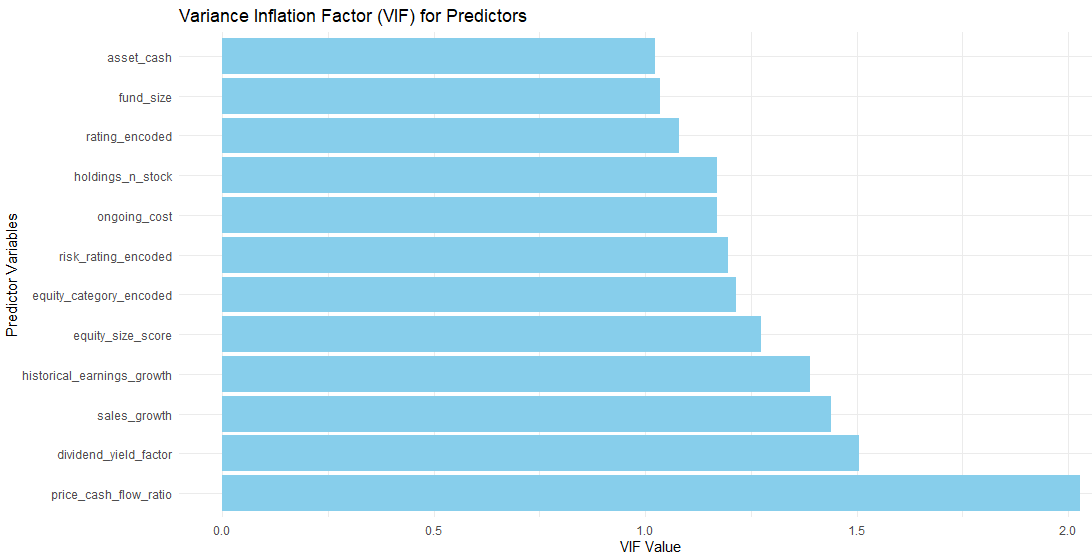
\includegraphics[width=0.8\textwidth]{Plots/VIF.png}
    \caption{VIF Values post Dataset Cleaning}
    \label{fig:vif}
\end{figure}

\begin{figure}[H]
    \centering
    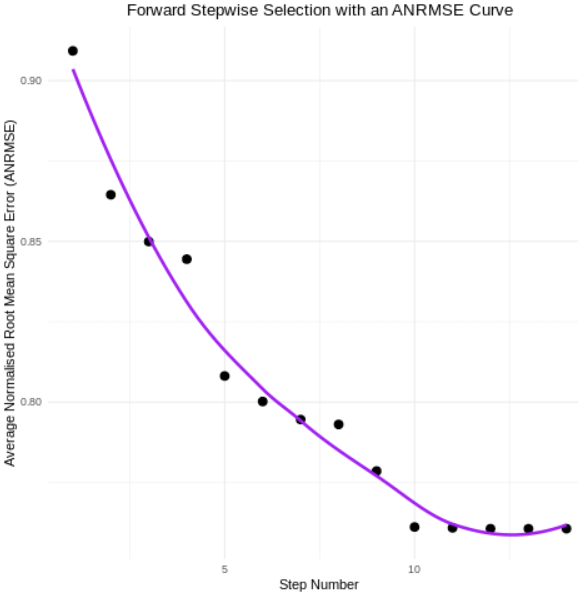
\includegraphics[width=0.5\textwidth]{Plots/Forward Stepwise Selection Plot.png}
    \caption{Forward Stepwise Selection with an ANRMSE Curve}
    \label{fig:fss}
\end{figure}

\section{Extra Chapter Insights}
\subsection{Introduction}
\subsubsection{Correlation Between Math Scores and Science Scores}
\label{Math Sci Cor}
\setlength{\tabcolsep}{4pt} % Adjust column spacing
\begin{table}[H]
    \centering
    \begin{tabular}{|c|c|c|c|}
        \hline
        \( X_1 \): Hours Studied & \( X_2 \): Time Spent on Papers & \( Y_1 \): Math Scores & \( Y_2 \): Science Scores\\
        \hline
        5  & 2  & 78 & 80 \\
        7  & 3  & 85 & 79 \\
        8  & 4  & 88 & 88 \\
        3  & 1  & 65 & 70 \\
        10 & 5  & 92 & 74 \\
        \hline
    \end{tabular}
    \caption{Study Time vs. Exam Scores}
    \label{tab:study_scoresA}
\end{table}

Let each pair \((x_i, y_i)\) represent Math (\(x\)) and Science (\(y\)) scores:
\[
\begin{aligned}
(x_1, y_1) = (78, 80),
(x_2, y_2) = (85, 79),
(x_3, y_3) = (88, 88),
(x_4, y_4) = (65, 70),
(x_5, y_5) = (92, 74).
\end{aligned}
\]
Next, compute the means. Let \(\bar{x}\) be the mean of the Math scores, and \(\bar{y}\) be the mean of the Science scores:

\[
\bar{x} = \frac{78 + 85 + 88 + 65 + 92}{5} = 81.6,\quad
\bar{y} = \frac{80 + 79 + 88 + 70 + 74}{5} = 78.2.
\]
For each pair \((x_i, y_i)\), compute \(\bigl(x_i - \bar{x}\bigr)\) and \(\bigl(y_i - \bar{y}\bigr)\). For clarity, the table below shows these values:

\[
\begin{array}{cccc}
\toprule
x_i & y_i & x_i - \bar{x} & y_i - \bar{y} \\
\midrule
78 & 80 & 78 - 81.6 = -3.6 & 80 - 78.2 = 1.8 \\
85 & 79 & 85 - 81.6 = 3.4  & 79 - 78.2 = 0.8 \\
88 & 88 & 88 - 81.6 = 6.4  & 88 - 78.2 = 9.8 \\
65 & 70 & 65 - 81.6 = -16.6 & 70 - 78.2 = -8.2 \\
92 & 74 & 92 - 81.6 = 10.4 & 74 - 78.2 = -4.2 \\
\bottomrule
\end{array}
\]
Next, multiply each pair of deviations and sum them:

\[
\sum_{i=1}^{5} (x_i - \bar{x})(y_i - \bar{y}) 
= (-3.6)(1.8) + (3.4)(0.8) + (6.4)(9.8) + (-16.6)(-8.2) + (10.4)(-4.2)= 151.4.
\]
Next, compute the Sum of Squares for Each Variable:
\[
\sum_{i=1}^{5} (x_i - \bar{x})^2
= (-3.6)^2 + (3.4)^2 + (6.4)^2 + (-16.6)^2 + (10.4)^2 = 449.2,
\]

\[
\sum_{i=1}^{5} (y_i - \bar{y})^2
= (1.8)^2 + (0.8)^2 + (9.8)^2 + (-8.2)^2 + (-4.2)^2 = 184.8.
\]
Finally, apply the Pearson Correlation Formula. The Pearson correlation coefficient \(r\) is given by
\[
r 
= 
\frac{\sum (x_i - \bar{x})(y_i - \bar{y})}
     {\sqrt{\sum (x_i - \bar{x})^2 \;\; \sum (y_i - \bar{y})^2}}
=
\frac{151.4}{\sqrt{449.2 \times 184.8}}
\approx 0.526.
\]
Thus, the correlation between the Math and Science scores in this dataset is approximately \(0.526\), indicating a moderate positive relationship.

\subsection{Exploratory Data Analysis}
\subsubsection{Mardia's Test for Multivariate Normality}
\label{Mardia's Test for MVN}

Mardia's test evaluates whether a set of multivariate data follows a multivariate normal distribution by examining two key properties: {multivariate skewness} and {multivariate kurtosis}.\cite{von2004testing}

The multivariate skewness statistic is defined as:
\[
\beta_{1,d} = \frac{1}{N^2} \sum_{i=1}^{N} \sum_{j=1}^{N} \left[ (x_i - \bar{x})^\top S^{-1} (x_j - \bar{x}) \right]^3,
\]
where \( x_i \) is the observation vector for the \( i \)-th observation, \( \bar{x} \) is the sample mean vector, \( S \) is the sample covariance matrix, \( N \) is the number of observations and \( d \) is the number of response variables.\cite{von2004testing}

Under the null hypothesis of multivariate normality, the skewness statistic \( \beta_{1,d} \) is asymptotically distributed as chi-squared with \( \frac{d(d+1)(d+2)}{6} \) degrees of freedom.\cite{von2004testing}
The p-value is calculated as:
\[
p = P\left( \chi^2_{\text{df}} > \beta_{1,d} \right),
\]
which corresponds to the upper-tail probability of the chi-squared distribution.


The multivariate kurtosis statistic is defined as:
\[
\beta_{2,d} = \frac{1}{N} \sum_{i=1}^{N} \left[ (x_i - \bar{x})^\top S^{-1} (x_i - \bar{x}) \right]^2,
\]
For a multivariate normal distribution, the expected value of \( \beta_{2,d} \) is \( d(d+2) \), and the variance is approximately:
\[
\text{Var}(\beta_{2,d}) = \frac{8d(d+2)}{N}.\cite{von2004testing}
\]
To assess deviation from normality, the kurtosis statistic is standardised:
\[
Z = \frac{\beta_{2,d} - d(d + 2)}{\sqrt{\text{Var}(\beta_{2,d})}}.
\]
The p-value is then computed from the standard normal distribution as:
\(
p = 2P(Z > |z|).
\)
This two-tailed test detects whether the kurtosis significantly deviates from the expected value under multivariate normality.

For the equity fund dataset, the sample covariance matrix is the response covariance matrix between ROE and sustainability score. $d=2$ because there are 2 responses and $N=1248$, which is the number of equity funds in the dataset.


\subsection{Multiple-Response Linear Regression}
\subsubsection{Covariance Expansion}
\label{Covariance Expansion}
\[
\text{Cov}(\mathbf{X} \mathbf{B}) = \text{E}[(\mathbf{X} \mathbf{B} - \text{E}[\mathbf{X} \mathbf{B}]) (\mathbf{X} \mathbf{B} - \text{E}[\mathbf{X} \mathbf{B}])^\top].
\]
Since expectation is linear: $\text{E}[\mathbf{X} \mathbf{B}] = \text{E}[\mathbf{X}] \mathbf{B}$, the centered term becomes: 
\[
(\mathbf{X} \mathbf{B} - \text{E}[\mathbf{X}] \mathbf{B}) = (\mathbf{X} - \text{E}[\mathbf{X}]) \mathbf{B}.
\]
Substitute this into the covariance definition:
\[
\text{Cov}(\mathbf{X} \mathbf{B}) = \text{E} \left[ (\mathbf{X} - \text{E}[\mathbf{X}]) \mathbf{B} \cdot (\mathbf{X} - \text{E}[\mathbf{X}])^\top \mathbf{B}^\top \right].
\]
Factor out \( \mathbf{B} \) because it is constant:
\[
\text{Cov}(\mathbf{X} \mathbf{B})=\mathbf{B}^\top \text{E} \left[ (\mathbf{X} - \text{E}[\mathbf{X}]) (\mathbf{X} - \text{E}[\mathbf{X}])^\top \right] \mathbf{B}.
\]
The middle term is just \( \text{Cov}(\mathbf{X}) \), therefore:
$
\text{Cov}(\mathbf{X} \mathbf{B}) = \mathbf{B}^\top \text{Cov}(\mathbf{X}) \mathbf{B}.
$

\subsection{Lasso and Ridge Regression}
\subsubsection{Closed-Form Coefficient Estimator Derivation}
\label{ridge-appendix}
We begin with the ridge regression loss function:
\begin{equation*}
\mathcal{L}(\boldsymbol{\beta}) = \| \mathbf{Y} - \mathbf{X} \boldsymbol{\beta} \|_2^2 + \lambda \| \boldsymbol{\beta} \|_2^2,
\end{equation*}
where \(\mathbf{X} \in \mathbb{R}^{n \times p}\), \(\mathbf{Y} \in \mathbb{R}^{n \times 1}\), and \(\boldsymbol{\beta} \in \mathbb{R}^{p \times 1}\).

To find the closed-form solution, we differentiate \(\mathcal{L}(\boldsymbol{\beta})\) with respect to \(\boldsymbol{\beta}\) and set the gradient equal to zero giving:
\begin{align*}
\nabla_{\boldsymbol{\beta}} \mathcal{L}(\boldsymbol{\beta}) 
    = -2 \mathbf{X}^\top (\mathbf{Y} - \mathbf{X} \boldsymbol{\beta}) + 2 \lambda \boldsymbol{\beta} &= 0, \\
\mathbf{X}^\top \mathbf{Y} 
    &= \mathbf{X}^\top \mathbf{X} \boldsymbol{\beta} + \lambda \boldsymbol{\beta}, \\
(\mathbf{X}^\top \mathbf{X} + \lambda \mathbf{I}) \boldsymbol{\beta} 
    &= \mathbf{X}^\top \mathbf{Y}.
\end{align*}

\noindent Hence, the closed-form solution for ridge regression is:
\begin{equation*}
\hat{\boldsymbol{\beta}}^{\text{Ridge}} = (\mathbf{X}^\top \mathbf{X} + \lambda \mathbf{I})^{-1} \mathbf{X}^\top \mathbf{Y}.
\end{equation*}
\noindent As desired.

\subsubsection{Multivariate Lasso Coordinate Descent Algorithm}
\label{multi-coord}

This algorithm comes from Liu et al. (2009) and its inputs are the standardised predictors, $\mathbf{X} \in \mathbb{R}^{n \times p}$, and standardised responses, $\mathbf{Y} \in \mathbb{R}^{n \times m}$, and the regularisation parameter $\lambda$.

\noindent First, initialise $\mathbf{B} = 0$ and carry out the following loop:

\begin{enumerate}
    \item For each predictor $j = 1, \dots, p$:
    \begin{enumerate}
        \item Compute the partial residual matrix for predictor $j$:
        \[
        \mathbf{R}_j = \mathbf{Y} - \sum_{k \neq j} \mathbf{X}_{\cdot k} \mathbf{B}_{k\cdot},
        \]
        where $\mathbf{X}_{\cdot k}$ is the $k$-th column of $\mathbf{X}$ and $\mathbf{B}_{k\cdot}$ is the $k$-th row of $\mathbf{B}$ (across all responses).
        
        \item Compute the least squares update for row $j$ (before thresholding):
        \[
        \mathbf{B}_{j\cdot}^* = \mathbf{X}_{\cdot j}^\top \mathbf{R}_j,
        \]
        giving a $1 \times m$ row vector.
        
        \item Apply element-wise soft-thresholding to update $\mathbf{B}_{j\cdot}$:
        \[
        \mathbf{B}_{j\cdot} \leftarrow \text{sign}(\mathbf{B}_{j\cdot}^*) \circ \left( |\mathbf{B}_{j\cdot}^*| - \lambda \right)_+,
        \]
        where $(z)_+ = \max(0, z)$ is applied element-wise, and $\circ$ denotes element-wise multiplication.
    \end{enumerate}
    \item Stop when:
    \[
    \|\mathbf{B}^{(k)} - \mathbf{B}^{(k-1)}\|_{\infty} < \epsilon_\text{Lasso},
    \]
    where $\epsilon_\text{Lasso}$ is the convergence threshold.\cite{liu2009blockwise}
\end{enumerate}

\noindent The output of this algorithm is the estimated coefficient matrix, $\hat{\mathbf{B}}$.


\subsection{Reduced Rank Ridge Regression}
\subsubsection{Minimisation Problem Simplification}
\label{Mini Simp}
Starting with the penalised objective:
\[
\| \mathbf{Y} - \mathbf{X} \mathbf{B} \|_F^2 + \lambda \| \mathbf{B} \|_F^2.
\]
The above is the sum of two Frobenius norms. Therefore, this can be written as a single Frobenius norm of a block matrix as follows:
\[
= \left\| 
\begin{pmatrix} 
\mathbf{Y} - \mathbf{X} \mathbf{B} \\ 
- \sqrt{\lambda} \mathbf{B} 
\end{pmatrix} 
\right\|_F^2.
\]
Now note that:
\[
\begin{pmatrix} 
\mathbf{Y} - \mathbf{X} \mathbf{B} \\ 
- \sqrt{\lambda} \mathbf{B} 
\end{pmatrix}
=
\begin{pmatrix}
\mathbf{Y} \\
\mathbf{0}
\end{pmatrix}
-
\begin{pmatrix}
\mathbf{X} \\
\sqrt{\lambda} \mathbf{I}
\end{pmatrix}
\mathbf{B}.
\]
Therefore, the penalised problem can be written as an equivalent least squares problem on an augmented dataset:
\[
\| \mathbf{Y} - \mathbf{X} \mathbf{B} \|_F^2 + \lambda \| \mathbf{B} \|_F^2 
= \left\| 
\begin{pmatrix} 
\mathbf{Y} \\ 
\mathbf{0} 
\end{pmatrix} 
- 
\begin{pmatrix} 
\mathbf{X} \\ 
\sqrt{\lambda} \mathbf{I} 
\end{pmatrix} \mathbf{B} 
\right\|_F^2=\| \mathbf{Y}^* - \mathbf{X}^* \mathbf{B} \|_F^2.
\]
Hence, the original penalised objective can be rewritten as the following unconstrained least squares objective on an augmented dataset:
\[
\hat{\mathbf{B}}(\lambda, r) = \underset{\text{rank}(\mathbf{B}) \leq r}{\arg\min} 
\;\| \mathbf{Y}^* - \mathbf{X}^* \mathbf{B} \|_F^2.
\]

\subsubsection{Mean Centring and the Response-Covariance Matrix}
\label{SVD Cov}
As a reminder, in general:
\[
\mathbf{\hat{\Sigma}_Y}=\frac{1}{n-1}(\mathbf{Y}-\bar{\mathbf{Y}})^\top (\mathbf{Y}-\bar{\mathbf{Y}})
\]
The response matrix \( \mathbf{Y} \) can be written as the sum of its mean-centred component and the mean matrix: $\mathbf{Y} = (\mathbf{Y} - \bar{\mathbf{Y}}) + \bar{\mathbf{Y}}.$
In this decomposition, \( \mathbf{Y} - \bar{\mathbf{Y}} \) is the mean-centred version of \( \mathbf{Y} \), while \( \bar{\mathbf{Y}} \) is a matrix where each row is the mean response vector \( \bar{\mathbf{y}} \).

Substituting the decomposition \( \mathbf{Y} = (\mathbf{Y} - \bar{\mathbf{Y}}) + \bar{\mathbf{Y}} \) into \( \mathbf{Y}^\top \mathbf{Y} \), gives $
   [(\mathbf{Y} - \bar{\mathbf{Y}}) + \bar{\mathbf{Y}}]^\top [(\mathbf{Y} - \bar{\mathbf{Y}}) + \bar{\mathbf{Y}}].$
Expanding this product results in
   \[
   \mathbf{Y}^\top \mathbf{Y} = (\mathbf{Y} - \bar{\mathbf{Y}})^\top (\mathbf{Y} - \bar{\mathbf{Y}}) + \bar{\mathbf{Y}}^\top (\mathbf{Y} - \bar{\mathbf{Y}}) + (\mathbf{Y} - \bar{\mathbf{Y}})^\top \bar{\mathbf{Y}} + \bar{\mathbf{Y}}^\top \bar{\mathbf{Y}}.
   \]
The two cross terms \( \bar{\mathbf{Y}}^\top (\mathbf{Y} - \bar{\mathbf{Y}}) \) and \( (\mathbf{Y} - \bar{\mathbf{Y}})^\top \bar{\mathbf{Y}} \) are equal to zero. This vanishing comes from the fact that the mean response matrix \( \bar{\mathbf{Y}} \) is constant across all rows, meaning that the sum of all deviations from the mean is equal to zero. Since:
   \[
   \sum_{i=1}^{n} (\mathbf{y}_i - \bar{\mathbf{y}}) = 0,
   \]
it follows that when multiplied by \( \bar{\mathbf{Y}} \), the result also vanishes:
\[
\sum_{i=1}^{n} \bar{\mathbf{y}}^\top (\mathbf{y}_i - \bar{\mathbf{y}}) = \bar{\mathbf{y}}^\top \sum_{i=1}^{n} (\mathbf{y}_i - \bar{\mathbf{y}}) = 0.\cite{jolliffe2002principal}
\]
Since this holds for all response variables, it means that $
   \bar{\mathbf{Y}}^\top (\mathbf{Y} - \bar{\mathbf{Y}}) = 0 \quad \text{and} \quad (\mathbf{Y} - \bar{\mathbf{Y}})^\top \bar{\mathbf{Y}} = 0.$
Substituting these results back into the expansion simplifies the equation to:
   \[
   \mathbf{Y}^\top \mathbf{Y} = (\mathbf{Y} - \bar{\mathbf{Y}})^\top (\mathbf{Y} - \bar{\mathbf{Y}}) + \bar{\mathbf{Y}}^\top \bar{\mathbf{Y}}.
   \]
The term \( \bar{\mathbf{Y}}^\top \bar{\mathbf{Y}} \) can be further simplified. Since each row of \( \bar{\mathbf{Y}} \) is equal to the mean response vector \( \bar{\mathbf{y}} \), and there are \( n \) such rows, the sum simplifies as follows:
\[
   \bar{\mathbf{Y}}^\top \bar{\mathbf{Y}} = n \bar{\mathbf{y}}^\top \bar{\mathbf{y}}.
\]
This scaling by \( n \) occurs because the same mean vector is repeated for all observations. Substituting this result into the equation gives:
\[
   \mathbf{Y}^\top \mathbf{Y} = (\mathbf{Y} - \bar{\mathbf{Y}})^\top (\mathbf{Y} - \bar{\mathbf{Y}}) + n \bar{\mathbf{Y}}^\top \bar{\mathbf{Y}}.\cite{jolliffe2002principal}
\]
This equation shows that \( \mathbf{Y}^\top \mathbf{Y} \) consists of the variance of the mean-centred data plus the contribution of the mean structure. In its final form, this is:
\[
\mathbf{Y}^\top\mathbf{Y} = (n-1)\mathbf{\hat{\Sigma}_Y}+n\mathbf{\bar{Y}}^\top\mathbf{\bar{Y}},
\]
where $\mathbf{\bar{Y}}^\top\mathbf{\bar{Y}}$ captures the mean effects of $\mathbf{Y}$. 

\subsubsection{Projection Simplification}
\label{proj}
Starting with:
\[
\left( \sum_{i=1}^{\tau} d_i \mathbf{u}_i \mathbf{v}_i^\top \right)
\left( \sum_{j=1}^{r} \mathbf{v}_j \mathbf{v}_j^\top \right)
= \sum_{i=1}^{\tau} d_i \mathbf{u}_i 
\left( \mathbf{v}_i^\top \sum_{j=1}^{r} \mathbf{v}_j \mathbf{v}_j^\top \right).
\]
The inner expression simplifies using orthonormality:
\begin{itemize}
  \item If \( i \leq r \): 
  \[
  \mathbf{v}_i^\top \sum_{j=1}^{r} \mathbf{v}_j \mathbf{v}_j^\top = \mathbf{v}_i^\top.
  \]
  \item If \( i > r \): 
  \[
  \mathbf{v}_i^\top \sum_{j=1}^{r} \mathbf{v}_j \mathbf{v}_j^\top = \mathbf{0}^\top.
  \]
\end{itemize}
\noindent So the entire sum becomes:
\[
\sum_{i=1}^{r} d_i \mathbf{u}_i \mathbf{v}_i^\top.
\]

\subsubsection{Singular Value Decomposition}
\label{RRR SVD}
Given the matrix \( \mathbf{\hat{Y}^*_R} \):
\[
\mathbf{\hat{Y}^*_R} =
\begin{bmatrix}
-5.67 & 2.96 & 4.19 & -14.29 & 12.81 & 0.74 & -0.62 \\
-1.82 & -0.91 & 2.28 & -2.73 & 3.19 & -0.23 & 0.55
\end{bmatrix}^{\top}.
\]
We aim to compute its Singular Value Decomposition: 
$
\mathbf{\hat{Y}^*_R} = \mathbf{U D V}^\top.
$
First, compute the Gram matrix:
\[
\hat{\mathbf{Y}}_R^*{}^\top \hat{\mathbf{Y}}_R^* =
\begin{bmatrix}
427.76 & 96.576 \\
96.58 & 27.34
\end{bmatrix}.
\]
This symmetric matrix is used to compute the eigenvalues and eigenvectors, which in turn provide the singular values. These singular values are the square roots of the eigenvalues of \( \hat{\mathbf{Y}}_R^*{}^\top \hat{\mathbf{Y}}_R^* \). The eigenvalues of \( \hat{\mathbf{Y}}_R^*{}^\top \hat{\mathbf{Y}}_R^* \) are: \( \lambda_1 = 449.84 \) and \( \lambda_2 = 5.26 \).

Hence:
\[
\mathbf{D} = 
\begin{bmatrix}
\sqrt{449.84} & 0 \\
0 & \sqrt{5.26}
\end{bmatrix}
=
\begin{bmatrix}
21.21   & 0 \\
0 & 2.29
\end{bmatrix}.
\]
The eigenvectors of \( \hat{\mathbf{Y}}_R^*{}^\top \hat{\mathbf{Y}}_R^* \) are the matrix \( \mathbf{V} \) (to 3sf):
\[
\mathbf{V} =
\begin{bmatrix}
0.975 & -0.223 \\
0.223 & 0.975
\end{bmatrix}.
\]
Now, we compute \( \mathbf{U} \) using the formula: $\mathbf{U} = \mathbf{\hat{Y}^*_R V S^{-1}}$.
Since \( \mathbf{V} \) is an orthonormal matrix, we have \( \mathbf{V}^\top = \mathbf{V}^{-1} \), giving (to 3sf):
\[
\mathbf{U} =
\begin{bmatrix}
-0.280 & 0.127 & 0.216 & -0.686 & 0.622 & 0.0316 & -0.0227 \\
-0.224 & -0.675 & 0.562 & 0.227 & 0.111 & -0.169 & 0.293
\end{bmatrix}^{\top}.
\]

\subsection{Multivariate Regression with Covariance Estimation}
\subsubsection{Negative Log-Likelihood Derivation}
\label{NLL}
Starting with the familiar MRLR model:
\[
\mathbf{Y}_{(n\times m)} = \mathbf{X}_{(n \times p)} \mathbf{B}_{(p \times m)} + \mathbf{E}_{(n \times m)},
\]
where $p$ no longer includes the column of ones.

Each row \( \mathbf{y}_i \in \mathbb{R}^{1 \times m} \) of \( \mathbf{Y} \) follows:
\[
\mathbf{y}_i|\mathbf{x}_i \sim \mathcal{N}_m(\mathbf{x}_i \mathbf{B}, \mathbf{\Sigma_E}),
\]
The probability density function for a single observation is:
\[
p(\mathbf{y}_i \mid \mathbf{x}_i) = \frac{1}{(2\pi)^{m/2} |\mathbf{\Sigma_E}|^{1/2}} \exp\left( -\frac{1}{2} (\mathbf{y}_i - \mathbf{x}_i \mathbf{B})^\top \mathbf{\Sigma_E}^{-1} (\mathbf{y}_i - \mathbf{x}_i \mathbf{B}) \right).
\]
Assuming independence across observations, the total log-likelihood becomes:
\begin{align*}
\log L(\mathbf{B}, \mathbf{\Sigma_E}) &= \sum_{i=1}^n \log p(\mathbf{y}_i \mid \mathbf{x}_i) \\
&= -\frac{nm}{2} \log(2\pi) - \frac{n}{2} \log |\mathbf{\Sigma_E}| - \frac{1}{2} \sum_{i=1}^n (\mathbf{y}_i - \mathbf{x}_i \mathbf{B})^\top \mathbf{\Sigma_E}^{-1} (\mathbf{y}_i - \mathbf{x}_i \mathbf{B})
\tag{*}
\end{align*}
Subbing the residual matrix, $\mathbf{E} = \mathbf{Y} - \mathbf{X} \mathbf{B}$, into the quadratic form gives:
\begin{align*}
\sum_{i=1}^n (\mathbf{y}_i - \mathbf{x}_i \mathbf{B})^\top \mathbf{\Sigma_E}^{-1} (\mathbf{y}_i - \mathbf{x}_i \mathbf{B}) &= \operatorname{tr} \left( \mathbf{E}^\top \mathbf{E} \mathbf{\Sigma_E}^{-1} \right)\\
&= \operatorname{tr} \left( (\mathbf{Y} - \mathbf{X} \mathbf{B})^\top (\mathbf{Y} - \mathbf{X} \mathbf{B}) \mathbf{\Omega} \right),
\end{align*}
where $\mathbf{\Omega} = \mathbf{\Sigma_E}^{-1}$.

Substituting back into (*), the log-likelihood becomes:
\[
\log L(\mathbf{B}, \mathbf{\Omega}) = -\frac{nm}{2} \log(2\pi) + \frac{n}{2} \log |\mathbf{\Omega}| - \frac{1}{2} \operatorname{tr} \left( (\mathbf{Y} - \mathbf{X} \mathbf{B})^\top (\mathbf{Y} - \mathbf{X} \mathbf{B}) \mathbf{\Omega} \right).
\]
Ignoring the constant term, \( \frac{nm}{2} \log(2\pi) \), the negative log-likelihood (NLL) becomes:
\[
\text{NLL}(\mathbf{B}, \mathbf{\Omega}) = \frac{1}{2} \operatorname{tr} \left( (\mathbf{Y} - \mathbf{X} \mathbf{B})^\top (\mathbf{Y} - \mathbf{X} \mathbf{B}) \mathbf{\Omega} \right) - \frac{n}{2} \log |\mathbf{\Omega}|.
\]
Finally, multiplying and dividing the trace term by \( n \), and omitting the constant \( \frac{1}{2} \), we obtain the simplified negative log-likelihood:
\[
g(\mathbf{B}, \mathbf{\Omega}) = \operatorname{tr} \left( \frac{1}{n} (\mathbf{Y} - \mathbf{X} \mathbf{B})^\top (\mathbf{Y} - \mathbf{X} \mathbf{B}) \mathbf{\Omega} \right) - \log |\mathbf{\Omega}|.
\]
This is the negative log-likelihood function (up to a constant) for the MRLR model.

\subsubsection{Proof of Algorithm 1}
\label{alg 1}
This proof comes from Rothman et al. (2010) and is as follows:

The objective function for $\mathbf{\Omega}$ fixed at $\mathbf{\Omega}_0$ (from Equation~\ref{B as Omega}), can be written more simply as:
\[
f(\mathbf{B}) = g(\mathbf{B}, \mathbf{\Omega}_0) + \lambda_2 \sum_{j=1}^{p} \sum_{k=1}^{q} |b_{jk}|,
\]
where:
\begin{equation*}
    g(\mathbf{B}, \boldsymbol{\Omega}_0) = \text{tr} \left[ \frac{1}{n} (\mathbf{Y} - \mathbf{X} \mathbf{B})^\top (\mathbf{Y} - \mathbf{X} \mathbf{B}) \boldsymbol{\Omega}_0 \right] - \log |\boldsymbol{\Omega}_0|.
\end{equation*}

\noindent First, solve for $\mathbf{B}$ with cyclical coordinate descent. Express the directional derivatives as:
\begin{align*}
\frac{\partial f^+}{\partial \mathbf{B}} &= \frac{2}{n} \mathbf{X}^\top \mathbf{X} \mathbf{B} \mathbf{\Omega} - \frac{2}{n} \mathbf{X}^\top \mathbf{Y} \mathbf{\Omega} + \lambda_2 \mathbf{1}(b_{ij} \geq 0) - \lambda_2 \mathbf{1}(b_{ij} < 0), \\
\frac{\partial f^-}{\partial \mathbf{B}} &= -\frac{2}{n} \mathbf{X}^\top \mathbf{X} \mathbf{B} \mathbf{\Omega} + \frac{2}{n} \mathbf{X}^\top \mathbf{Y} \mathbf{\Omega} - \lambda_2 \mathbf{1}(b_{ij} > 0) + \lambda_2 \mathbf{1}(b_{ij} \leq 0),
\end{align*}
where the indicator $\mathbf{1}()$ is understood to be a matrix. Let $\mathbf{S} = \mathbf{X}^\top \mathbf{X}$ and $\mathbf{H} = \mathbf{X}^\top \mathbf{Y} \mathbf{\Omega}$, and define:
\[
u_{rc} = \sum_{j=1}^{p} \sum_{k=1}^{q} b_{jk} s_{rj} \omega_{kc}.
\]
Next, update a single parameter $b_{rc}$, using the directional derivatives:
\begin{align*}
\frac{\partial f^+}{\partial b_{rc}} &= u_{rc} - h_{rc} + n \lambda_2 \mathbf{1}(b_{ij} \geq 0) - n \lambda_2 \mathbf{1}(b_{ij} < 0), \\
\frac{\partial f^-}{\partial b_{rc}} &= -u_{rc} + h_{rc} - n \lambda_2 \mathbf{1}(b_{ij} > 0) + n \lambda_2 \mathbf{1}(b_{ij} \leq 0).
\end{align*}
\noindent Let $b_{rc}^0$ be the current iterate. The unpenalised univariate minimised, $\hat{b}^*_{rc}$, solves:
\[
\hat{b}^*_{rc} s_{rr} \omega_{cc} - b_{rc}^0 s_{rr} \omega_{cc} + u_{rc} - h_{rc} = 0,
\]
implying:
\[
\hat{b}^*_{rc} = b_{rc}^0 + \frac{h_{rc} - u_{rc}}{s_{rr} \omega_{cc}}.
\]
If $\hat{b}^*_{rc} > 0$, then we look leftward, and by convexity, the penalised minimiser is:
\[
\hat{b}_{rc} = \max\left(0, \hat{b}^*_{rc} - \frac{n \lambda_2}{s_{rr} \omega_{cc}}\right).
\]
Similarly, if $\hat{b}^*_{rc} < 0$ then we look to the right, and by convexity, the penalised univariate minimiser is:
\[
\hat{b}_{rc} = \min\left(0, \hat{b}^*_{rc} + \frac{n \lambda_2}{s_{rr} \omega_{cc}}\right).
\]
Thus,
\[
\hat{b}_{rc} = \text{sign}(\hat{b}^*_{rc})\left( |\hat{b}^*_{rc}| - \frac{n \lambda_2}{s_{rr} \omega_{cc}} \right)_+.
\]
Also, if $\hat{b}^*_{rc} = 0$, which has probability zero, then both the loss and penalty part of the objective function are minimised and the parameter stays at 0. We can write this solution compactly as:
\[
\hat{b}_{rc} = \text{sign}\left( b_{rc}^0 + \frac{h_{rc} - u_{rc}}{s_{rr} \omega_{cc}} \right) \left( \left| b_{rc}^0 + \frac{h_{rc} - u_{rc}}{s_{rr} \omega_{cc}} \right| - \frac{n \lambda_2}{s_{rr} \omega_{cc}} \right)_+.\cite{rothman2010sparse}
\]
As desired.

\vspace{-0.2cm}
\subsubsection{Graphical Lasso Form}
\label{glasso}
First, let us justify why glasso works using its setup and how MRCE corresponds. The glasso setup, from Friedman et al. (2008), begins as follows: you have an observed data matrix $\mathbf{Z}$, where $\mathbf{Z}\in\mathbb{R}^{n \times m}$. These vectors are assumed to be drawn from a multivariate Gaussian distribution \(\mathcal{N}(\mathbf{0}, \boldsymbol{\Sigma})\), where \(\boldsymbol{\Sigma}\) is the \(m \times m\) covariance matrix.

The aim of glasso is to estimate the precision matrix, \(\boldsymbol{\Omega} = \boldsymbol{\Sigma}^{-1}\).
Glasso estimates \(\boldsymbol{\Omega}\) by solving the following optimisation problem:
\begin{equation}
\text{arg}\max_{\boldsymbol{\Omega} \succ 0} \{ \log |\boldsymbol{\Omega}| - \operatorname{tr}(\mathbf{S} \boldsymbol{\Omega}) - \lambda \|\boldsymbol{\Omega}\|_1 \},
\label{glasso optimisation}
\end{equation}
where $\lambda > 0$ is the regularisation parameter, \(\|\boldsymbol{\Omega}\|_1 = \sum_{j,k} |\omega_{jk}|\) and \(\mathbf{S}\) is the empirical covariance matrix, computed as \(\mathbf{S} = \frac{1}{n} \mathbf{Z}^\top \mathbf{Z}\).\cite{friedman2008sparse}

\noindent MRCE uses the glasso setup to estimate the inverse error covariance matrix, \(\boldsymbol{\Omega}=\mathbf{\Sigma_E}\), for the errors in MRLR because the errors \(\mathbf{E}_i \sim \mathcal{N}(\mathbf{0}, \mathbf{\Sigma_E})\) match the Multivariate Gaussian assumption of glasso. Its optimisation problem, for $\mathbf{\Omega}$, can also be rewritten in the form of Equation~\ref{glasso optimisation}. 

Here is Equation~\ref{Omega as B}, the optimisation problem, for $\mathbf{\Omega}$, again:
\begin{equation*}
    \hat{\boldsymbol{\Omega}}(\mathbf{B}_0) = \arg \min_{\boldsymbol{\Omega}} \left\{ \text{tr} \left[ \hat{\mathbf{\Sigma}}_R \boldsymbol{\Omega} \right] - \log |\boldsymbol{\Omega}| + \lambda_1 \sum_{j' \neq j} |\omega_{j'j}| \right\},
\end{equation*}
\noindent where $\hat{\mathbf{\Sigma}}_R=\frac{1}{n} (\mathbf{Y} - \mathbf{X} \mathbf{B}_0)^\top (\mathbf{Y} - \mathbf{X} \mathbf{B}_0)$.
\[
\arg\min_{\mathbf{\Omega}} \left\{ \mathrm{tr}( \hat{\mathbf{\Sigma}}_R\, \mathbf{\Omega} ) - \log|\mathbf{\Omega}| + \lambda_1 \sum_{i \ne j} | [\mathbf{\Omega}]_{ij} | \right\}
=
\arg\max_{\mathbf{\Omega} \succ 0} \left\{ \log|\mathbf{\Omega}| - \mathrm{tr}( \hat{\mathbf{\Sigma}}_R\, \mathbf{\Omega} ) - \lambda_1 \| \mathbf{\Omega} \|_1 \right\},
\]
which comes from the rule for argmin and argmax that:
\[
\arg\max_x f(x) = \arg\min_x \left[ -f(x) \right]
\]
This gives the graphical-lasso form:
\[
\hat{\mathbf{\Omega}}( \mathbf{B}_0 )
= \arg\max_{\mathbf{\Omega} \succ 0}
\left\{
\log|\mathbf{\Omega}| - \mathrm{tr}( \hat{\mathbf{\Sigma}}_R\, \mathbf{\Omega} ) - \lambda_1 \| \mathbf{\Omega} \|_1
\right\},
\quad \text{where } \| \mathbf{\Omega} \|_1 = \sum_{i \ne j} \left| \mathbf{\Omega}_{ij} \right|.
\]
%\vspace{-0.1cm}
This setup allows MRCE to account for correlations among the errors of the \(m\) responses.
%\subsection{Covariance-Regression with Random Forests}
%\vspace{-0.1cm}
\subsection{Cholesky-Gaussian XGBoost}
%\vspace{-0.1cm}
\subsubsection{Weighted Quantile Sketches}
\label{WQS}
In the approximate split-finding algorithm, as already stated, candidate split points are chosen based on percentiles of the feature values. The rank function \( r_k(z) \) calculates the proportion of instances where feature \( k \) is less than \( z \), weighted by second-order gradient statistics \( h \).\cite{chen2016xgboost} The algorithm aims to find split points \( s_{k1}, s_{k2}, \dots, s_{kl} \) such that the difference between the ranks of consecutive points is small, controlled by \( \epsilon \), which is an approximation factor.\cite{chen2016xgboost} This process ensures that the split points are well-distributed across the range of the feature values.

The Hessian, \( h_i \), is used as a weight for each instance or row in the dataset, meaning that data points with larger Hessians carry more influence in determining the split. This weighting reflects the importance of the instance in minimising loss. Higher-weighted instances show where the model struggles, guiding the algorithm to focus on these critical areas during split finding.

Traditional quantile sketch algorithms work for datasets where all instances have equal weights.\cite{chen2016xgboost} However, no existing algorithm efficiently handles weighted data, which creates challenges in approximating split points for datasets with imbalanced or sparse data distributions. Randomised sorting or heuristic approaches have been used to address this issue, but these methods lack theoretical guarantees.\cite{chen2016xgboost} As a result, they may fail to identify the optimal split points, leading to suboptimal model performance. To overcome this limitation, XGBoost introduces a novel weighted quantile sketch algorithm that can handle weighted data with provable theoretical guarantees.\cite{chen2016xgboost} This algorithm ensures accurate split findings by accounting for the distribution of weights across the dataset. %improving performance on imbalanced data.
%\vspace{-0.3cm}
\subsubsection{Cholesky-Decomposition Verification}
\label{CD}
Verification occurs by computing:
\begin{align*}
\mathbf{L} \mathbf{L}^\top 
&= 
\begin{bmatrix}
2 & 0 \\
1 & \sqrt{2}
\end{bmatrix}
\begin{bmatrix}
2 & 1 \\
0 & \sqrt{2}
\end{bmatrix} 
=
\begin{bmatrix}
(2)(2) + (0)(0) & (2)(1) + (0)(\sqrt{2}) \\
(1)(2) + (\sqrt{2})(0) & (1)(1) + (\sqrt{2})(\sqrt{2})
\end{bmatrix} \\[10pt]
&=
\begin{bmatrix}
4 & 2 \\
2 & 3
\end{bmatrix}
= \mathbf{A}.
\end{align*}
\noindent As desired.


%\subsubsection{Further Calculations}

%\section{Stepwise Selection Code}

\end{document}
